\documentclass[a4paper,11pt]{refrep}
\input{xcsoar.sty}

% Set the title
\title{User Manual}

% Set the page title
\input{xcsoar-headers.sty}
\xcsoarheader{XCSoar User Manual}

\def\maketitle{%
  \null
  \thispagestyle{empty}%
  \begin{maxipage}
    \begin{center}
    
\includegraphics[angle=0,width=0.5\textwidth,keepaspectratio='true']{graphics/logo.png}
    \vskip 0.5cm
    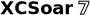
\includegraphics[angle=0,width=0.66\textwidth,keepaspectratio='true']{graphics/title.pdf}
    \end{center}
    \begin{center}
      \normalfont\huge\textsf{the open-source glide computer}\par
    \end{center}
    \vskip 1cm
    \begin{center}
      \normalfont\huge\textsf{\@title}\par
    \end{center}
    \vskip 1cm
  \end{maxipage}

  \vfill
  \todo[nolist,size=\Large,inline]{Draft state, better you wait printing the
  whole manual}

  \begin{flushright}
    \large \strut {
      \sf
      \today \\
      For XCSoar version \version \\
      \xcsoarwebsite{} \\
    } 
    \par
  \end{flushright}
  \par
  \vfil
  \vfil
  \null
  \cleardoublepage
}

\usepackage{makeidx}\makeindex

\begin{document}

%%%%%%%%%%%%%%%%%%%%%%
% Front page
\maketitle

%%%%%%%%%%%%%%%%%%%%%%
% Table of contents
\input{toc.tex}

%%%%%%%%%%%%%%%%%%%%%%
\chapter*{Preface}

\section*{Warnings and precautions}

\warning IT IS THE USER'S RESPONSIBILITY TO USE THIS SOFT\-WARE PRUDENTLY. THIS SOFTWARE IS 
INTENDED TO BE USED ONLY AS A NAVIGATION AID AND MUST NOT BE USED FOR ANY PURPOSE REQUIRING 
PRECISE MEASURE\-MENT OF DIRECTION, DISTANCE, LOCATION, OR TOPO\-GRAPHY. THIS SOFTWARE SHOULD 
NOT BE USED AS AN AID TO DETERMINE GROUND PROXIMITY FOR AIRCRAFT NAVIGATION. THIS SOFTWARE 
SHOULD NOT BE USED AS A TRAFFIC COLLISION AVOIDANCE SYSTEM.



%%%%%%%%%%%%%%%%%%%%%%
\section*{Legal notices}

\subsection*{Software license agreement}

This software is released according to the GNU General Public License
Version~2.  See Appendix~\ref{cha:gnu-general-public} for the full
text of the agreement and warranty notice.

\subsection*{Limited liability}

In no event shall XCSoar, or its principals, shareholders, officers,
employees, affiliates, contractors, subsidiaries, or parent
organizations, be liable for any incidental, consequential, or
punitive damages whatsoever relating to the use of the Product.

\subsection*{Disclaimer}
This product, and all accompanying files, data and materials, are
distributed ``as is'' and with no warranties of any kind, whether
express or implied.  This product is used entirely at the risk of the
user.  Although great care has been taken to eliminate defects during
its development it is not claimed to be fault-free. No claims are made
regarding its correctness, reliability or fitness for any particular
purpose.  The XCSoar project developers and contributors shall not be
liable for errors contained herein or for incidental or consequential
damages, loss of data or personal injury in connection with
furnishing, performance, or use of this material.


%%%%%%%%%%%%%%%%%%%%%%
\chapter{Introduction}\label{cha:introduction}
Questo è il manuale del pilota di XCSoar, un computer di volo open-source
originalmente sviluppato per i dispositivi Pocket PC devices.  Si presume 
che l'utente abbia un solida conoscenza della teoria del volo veleggiato,
e come minimo una conoscenza basilare del volo di cross-country.

Gli aggiornamenti al software di XCSoar potrebbero rendere questo manuale 
obsoleto. Si raccomanda di leggere le note di rilascio distribuite con il 
software per tenere tracia dei cambiamenti.  Aggionamenti a manuale e software
sono disponibili su 
\begin{quote}
\xcsoarwebsite{}
\end{quote}

\section{Organizazione di questo manuale}

\todonum[inline]{Write about the manual crossref hinting icons and the yellow
colour. The Quickstart will be readable also without those links available} 
Questo manuale è scritto particolarmente per permettere all'utente di XCSoar
un rapido utilizzo, 
  \emph{così come} supportare una profonda comprensione di tutte le funzioni, 
concetti e tattiche introdotte. Gli autori hanno fatto tutto il possibile per 
farlo dalla prospettiva del pilota (e onestamente sperano di esserci riusciti).

Gli autori suggeriscono vivamente di prendersi il tempo di leggere a fondo
tutto il manuale, capitolo per capitolo (con l'eccezione dei capitoli di 
riferimento Infobox e Configurazione). È garantito che il tempo speso si
ripagherà sotto forma di comprensione. Durante la lettura potrà capitare di 
sentirsi un po' persi ogni tanto, per questo motivo gli autori hanno inserito
link ed icone.

\begin{figure}[h]
\centering
\includegraphics[width=0.8cm,angle=0,keepaspectratio='true']{figures/config.pdf}
\hspace{1.5cm}
\includegraphics[width=0.8cm,angle=0,keepaspectratio='true']{figures/reminder.pdf}
\hspace{1.5cm}
\includegraphics[width=0.8cm,angle=0,keepaspectratio='true']{figures/gesture.pdf}
\hspace{1.5cm}
\includegraphics[width=0.8cm,angle=0,keepaspectratio='true']{figures/warning.pdf}
\caption{Icons configuration, reminder, gesture, warning}
\end{figure}

\warning Avvertimento. L'icona di avvertimento è usata ovunque le cose vadano 
seguite esattamente. Non farlo potrebbe causare risultati inattesi, disfunzioni
totali o addirittura pericolo per l'incolumità. Procedere solo se si è compreso
il pericolo.

\gesture{DU} Gesto. Nei dispositivi dotati di touch-screen, un gesto di scorrimento
può essere usato per invocare il menu o una funzione piuttosto che un'altra.
In questo esempio, DU sta per muovere il dito verso il basso e poi verso l'alto
(in linee diritte) sullo schermo.
  
\gesturespec{du} Gesto Specifico. Ovunque l'auore abbia tentuto il passo con il rapido sviluppo di XCSoar, è fornita un'icona specifica che illustri i movimenti.

\tip Promemoria. Questa icona rappresenta un suggerimenti, un trucco, cose che dovresti ricordare dopo aver letto la sezione corrispondente e così via.

\config{orientation} Vedi configurazione ... L'icona che rappresenta du e attrezzi
da officina rimanda ad un approfondimento degli elementi menzionati e come configurarli. I numeri accanto all'icona si riferiscono agli specifici capitoli/sezioni di riferimento di questo manuale \ref{cha:infobox} e 
\ref{cha:configuration}, in questo caso si riferiscono ad una sezione \ref{conf:orientation}. 

\marginlabel{\parbox{1.3cm}{\rotatebox[origin=c]{180}{\includegraphics[width=0.9cm]{figures/warning.pdf}}}}
\rotatebox[origin=c]{180}{Smetti di leggere il manuale mentre stai volando all'indietro!}

\emph{Leggi} a casa, \emph{configura} al suolo, in sicurezza. Se hai percepito questo avvertimento (invertito) 
come un esempio, sei pronto a procedere.

\config{usingxcsoarsafely} In riferimento alla seconda icona di esempio 
``configurazione'' a sinistra, l'icona punta al capitolo \ref{cha:introduction}, (questo capitolo), sezione 
\ref{sec:usingxcsoarsafely}, ``Usare XCSoar in sicurezza'' sotto, che potrebbe essere
intesa come ``come configurare te stesso''. Sta a te decidere se tuffarti in una discussione
approfondita e poi tornare indietro, oppure semplicemente procedere. Se stai leggendo il manuale in 
forma elettronica, cliccare il numero ti farà saltare al riferimento incrociato richiesto.
Usa la funzione ``indietro'' (o simili) del tuo browser per tornare sul capitolo da cui eri saltato.

I numeri stampati in blu, così come le icone appena introdotte, indicano ``aiuto
disponibile''. Lo stesso vale per gli altri URL e testi blu sottostanti.
Cliccare su un testo come \xcsoarwebsite{/contact} aprità il tuo browser web 
o l'applicazione di posta elettronica per metterti in contatto rispettivamente
con altre risorse o gente più esperta.

Il resto di questo capitolo ``Introduzione'' è riguardo a renderti preparato
per XCSoar, come aumentare il tuo livello di comprensioe e coltivare  le tue capacità. 
Il capitolo \ref{cha:quickstart} ``Quickstart'' potrebbe essere la prossima boa dopo
\ref{cha:installation} ``Installazione'' per gli utenti frettolosi. Sentiti libero di 
tagliar corto, ma non disdegnare di leggere tutto capitolo per capitolo, seguendo:

Il capitolo~\ref{cha:interface} introduce i concetti dell'interfaccia utente
e fa una panoramica del display.

Il capitolo~\ref{cha:navigation} descrive in gran dettaglio la mappa mobile
e come il software possa assistere nella navigazione generale.

Il capitolo~\ref{cha:tasks} descrive come sono specificate e volate le task
di cross-country, e presenta alcuni degli strumenti di analisi disponibili
pe ri piloti per aiutarli a migliorare le proprie prestazioni.

Il capitolo~\ref{cha:glide} scende in maggior dettaglio nelle funzioni del computer
di volo, perchè è importante per i piloti essere a conoscenza di come questo 
esegua i suoi calcoli.

Il capitolo~\ref{cha:atmosph} spiega come il computer si possa
interfacciare con variometri ed altri sensori di dati dell'aria
e come usa questi dati per fornire vari modelli dell'atmosfera, in
particolare su vento e convezione termica.

Il capitolo~\ref{cha:airspace} descrive come XCSoar può assistere 
nella gestione del volo in determinati airspace ed il sistema
anticollisione FLARM.

Il capitolo~\ref{cha:avionics-airframe} riguarda integrazione
 di sistema e diagnostiche, l'integrazione di XCSoar con
dispositivi di comunicazione e interruttori del velivolo.

Il resto del manuale contiene principalmente materiale di riferimento.
Il capitolo~\ref{cha:infobox} elenca i tipi di informazione che possono
essere mostrati nella griglia di InfoBox accanto alla mappa.
La configurazione del software è descritta in dettaglio nel capitolo~\ref{cha:configuration}.
I formati dei faile dati usati dal programma, come ottenerli
e come modificarli, è descritto nel capitolo~\ref{cha:data-files}.

Infine, una breve storia e discussione del processo di sviluppo di XCSoar
è presentata nel capitolo~\ref{cha:history-development}.

\section{Note}

\subsection*{Screenshot}
In tutto il manuale ci sono diversi screenshot di XCSoar. Questi sono presi
dal programma in funzione su una varietà di piattaforme hardware e probabilmente
anche versioni differenti. Ogni piattaforma potrebbe avere differente risoluzione
dello schermo, layout e caratteri, quindi ci possono essere leggere differenze 
nell'aspetto del display. La maggior parte degli screenshot in questo manuale
sono presi con XCSoar in configurazione orizzontale.

\section{Piattaforme}
\begin{description}
\item[Dispositivi Android]
XCSoar funziona su Android 1.6 o successivi.
\item [eBookreader]
XCSoar funziona su diversi modelli di eReader Kobo.
\item[PC Windows]
È possibile far funzionare XCSoar su un qualsiasi computer con sistema
operativo Windows (Vista e successivi). 
Questo setup può essere usato per allenarsi ad usare XCSoar.
Nel software sono presenti una modalità simulazione ed una funzione
di replay delle tracce IGC che possono essere usate in assenza di un
dispositivo GPS valido.
\item[Unix/Linux PC]
XCSoar funziona su Unix/Linux.
\end{description}



\section{Supporto tecnico}

\subsection*{Troubleshooting}
XCSoar è prodotto da un piccolo team di sviluppatori dedicati. Sebbene siamo
felici di aiutare con l'utilizzo del software, non possiamo insegnarti le basi 
della moderna tecnologia informatica. Se hai una particolare domanda su XCSoar 
non presente in questo manuale, per favore mettiti in contatto.
Troverai tutti i seguenti link riassunti su:
\begin{quote}
\xcsoarwebsite{/contact}
\end{quote}
Per cominciare con la comunicazione, unisciti al forum di XCSoar:
\begin{quote}
\url{http://forum.xcsoar.org}
\end{quote}
Se i tuoi dubbi non sono già stati affrontati, postali o scrivici: 
\begin{quote}
\href{mailto:xcsoar-user@lists.sourceforge.net}{xcsoar-user@lists.sourceforge.net}
\end{quote}
Le domande frequenti verranno aggiunte a questo documento.
Potresti anche trovare utile iscriverti alla mailing-list degli utenti di XCSoar,
in modo di essere sempre aggiornato sugli ultimi sviluppi.

Se niente di tutto questo è sufficiente, probabilmente hai scoperto un bug.

\subsection*{Feedback}
Come ogni programma software complesso, XCSoar può essere soggetto a
bug, quindi se ne trovi qualcuno per favore riportalo agli sviluppatori
usando il nostro portale di bug tracking: 
\begin{quote}
\xcsoarwebsite{/develop/new_ticket.html}
\end{quote}
o inviando una mail a:
\begin{quote}
\href{mailto:xcsoar-devel@lists.sourceforge.net}{xcsoar-devel@lists.sourceforge.net}
\end{quote}
XCSoar registra molti dati valevoli in un file di log
\verb|xcsoar.log| nella directory \texttt{XCSoarData}. Il file di log può essere aggiunto alla segnalazione del bug per aiutare gli sviluppatori a determinare la causa del problema.
Se ti piace l'idea di fare qualcosa di più, fatti coinvolgere:
\begin{quote}
\xcsoarwebsite{/develop}
\end{quote}

\subsection*{Aggiornamenti}
È consigliato visitare periodicamente il sito di XCSoar per controllare
se ci sono aggiornamenti del programma.
La procedura di installazione descritta nel capitolo seguente può essere 
ripetuta per aggiornare il software.
Tutte le configurazioni utente e file di dati saranno preservate durante
l'aggiornamento o la reinstallazione.

È anche consigliato di controllare periodicamente se ci sono aggiornamenti
per i file dei dati, specialmente quelli degli spazi aerei, che potrebbero
essere soggetti a cambiamenti dalle autorità di aviazione civile nazionali.

\section{Allenamento}
Per la sicurezza propria e degli altri, ai piloti è consigliato di allenarsi
a terra all'uso di XCSoar, in modo da familiarizzare con l'interfaccia e le
funzioni prima di volare.

\subsection*{Usare XCSoar sul PC}
La versione per PC può essere usata per familiarizzare con l'interfaccia
e le funzionalità di XCSoar nel comfort della propria casa. Tutti i file e
le configurazioni usate da questa versione sono identici alle versioni embedded,
quindi può essere utile provare le personalizzazioni al PC prima di usarle
in volo.

La versione da PC può anche esser collegata a dispositivi esterni e funzionare
esattamente come la versione embedded. Utilizzi suggeriti sono:
\begin{itemize}
\item Connettere il PC ad un dispositivo FLARM per usare XCSoar come una
stazione a terra, per visualizzare il traffico FLARM.
\item Connettere il PC ad un variometro intelligente, come il Vega, per provare
le impostazioni del variometro.
\end{itemize}

\subsection*{Usare XCSoar con un simulatore di volo}
Un buon modo di imparare a dusare XCSoar è di connettere uno smartphone
ad un PC con un simulatore di volo che possa produrre sentenze NMEA
attraverso la porta seriale.
Simulatori di volo adatti sono Condor e X-Plane.  

I benefici di questa forma di allenamento sono che XCSoar può essere usato
in modalità FLY, così si comporta esattamente come se si stesse realmente
volando, e si può ottenere una buona impressione di come il programma lavori
mentre si vola nel simulatore.

\section{Usare XCSoar in sicurezza}\label{sec:usingxcsoarsafely}\label{conf:usingxcsoarsafely}
L'uso di un sistema interattivo come XCSoar in volo comporta un certo
rischio dovuto alla potenziale distrazione del pilota dal mantenimento
della consapevolezza della situazione e dal tenere d'occhio i dintorni.

La filosofia dietro design e sviluppo del software è di tentare di ridurre
il più possibile queste distrazioni minimizzando la necessità di interazione
da parte dell'utente, e presentando le informazioni in modo chiaro ed
interpretabile con uno sguardo.

I pilot che usano XCSoar devono prendersi la responsabilità di usare il
sistema in sicurezza.
Buone pratiche nell'uso di XCSoar includono:
\begin{itemize}
\item Familiarizzare col sistema attraverso intenso allenamento a terra.
\item Effettuare manovre di allontanamento prima di interagire con XCSoar
  in volo, per assicurarsi che non ci sia rischio di collisione con altro traffico.
\item Impostare il sistema in modo da trarre vantaggio dalle funzioni automatiche
  e dagli eventi in ingresso, in modo che le interazioni utente siano mimimizzatee.
  Se ti accorgi di ripetere meccanicamente certe azioni, chiediti (o chied ad altri
  utenti) se il software non possa gestire queste interazioni per te.
\end{itemize}


%%%%%%%%%%%%%%%%%%%%%%
\chapter{Installation}\label{cha:installation}

\section{To run XCSoar}
 you need to obtain the following:

\begin{itemize}
\itemsep0em
\item a device to run XCSoar on
\item XCSoar
\item a GPS receiver
\item a waypoint file
\item an airspace file (optional)
\item a map file (optional)
\end{itemize}

\section{! Before you go out flying the first time with XCSoar !}

After having installed XCSoar successfully, you might use it instantly. XCSoar 
will launch with a ready-to-use pre-configuration. But be aware, that up to 
this point your new toy will give you a moving map display only.
\warning \emph{Don't trust the computations.} You have to tell XCSoar which 
plane you are flying in advance.  This is done by specifying your plane's data 
as are polar, weight and some other data.  However it's always a good idea to 
study the manual and become familiar with XCSoar at home.

\section{How to get the most from XCSoar}

In order to achieve your maximum benefit from XCSoar, you are kindly asked to 
do some more after having installed the software and downloaded some data
files. ``Some more'' includes personal and plane data as well as configuration 
of just a few features. Unless you are willing to tweak everything XCSoar 
provides, this could be done in a rather short time. Necessary steps are 
summarized in an \emph{XCSoar Checklist}, given in the next section.

If you are planning to arrange a system with several components engaged in, 
this manual will give you valuable advice on both, how to set up things and how 
to use them.

If you are a pilot in a hurry, the authors suggest to change to the short form 
manual \texttt{XCSoar-in-a-Flash} going through the \emph{XCSoar Checklist} 
step by step. The short form manual is available on \url{http://www.xcsoar.org/
discover/manual.html}.



\section{XCSoar Checklist}

\subsection*{{Bring XCSoar into play}}
\begin{itemize}
\item get hardware and install XCSoar
\item get appropriate data files of your flight district
\item tell XCSoar which data files to use
\item tell XCSoar about the glider's polar \& weight
\item possibly connect to instruments
\item finish setup and familiarize
\item mount hardware
\item add items listed underneath to your checklists
\item make ``home''
\end{itemize}

\subsection*{Conduct preflight check, including}
\begin{itemize}
\item setup polar and weight
\item setup wind and flight parameters (MC, bugs, QNH)
\item possibly setup a task
\end{itemize}

\subsection*{Conduct start check, including}
\begin{itemize}
\item Check wind and flight setup once more
\end{itemize}
\vspace{2em}

\subsection*{Fly, enjoy}
\vspace{4em}

\subsection*{Conduct after flight check}
\begin{itemize}
\item Download flight logs from logger, upload to skylines and OLC
\item Gather statistical data of flight.
\end{itemize}
\newpage




\section{Compatibility}

\subsection*{Devices for running XCSoar}

XCSoar runs on the following platforms:

\begin{itemize}
\item Android mobile phones and tablets with Android 1.6 or newer \\
  Example: Dell Streak, Samsung Galaxy S II, HTC Desire HD,
  Motorola Xoom
\item eReader Kobo
\item Windows 2000 or newer
\item Linux
\item Mac OS X (outdated)
\end{itemize}

\subsection*{GPS, Logger, Vario}

XCSoar is compatible with any GPS emitting NMEA data.  Most modern
Android devices have a built-in GPS, but for several reasons it is favorable to
connect to one or more external devices:

\begin{itemize}
\item a specialized GPS receiver gains much better reception providing much 
better data for measures and calculations
\item an airspeed indicator allows quick and exact wind estimates
  without circling
\item a vario improves the thermal assistant
\item a task can be declared to an IGC logger, and after landing, the
  flight log can be downloaded
\item some varios allow synchronising the MacCready setting with
  XCSoar
\item FLARM (and even ADS-B input) provide informations and states of others
around you (and of course FLARM gives you collision detection)
\end{itemize}

\subsection*{Supported external devices and features}
\label{sec:supported-varios}

\newcommand{\y}[0]{{ $\surd$ }}
%{0.8\textwidth}
\noindent\makebox[\textwidth]{%
\begin{tabular}{l|ccc|cc|cc|c}
       \multicolumn{1}{r}{Supported:} & \multicolumn{3}{c|}{-Features} & \multicolumn{5}{c}{-Stream Data} \\
NMEA Device & 
  \begin{sideways} Declaration\end{sideways} & 
  \begin{sideways} Remote ctrl.\end{sideways} & 
  \begin{sideways} Download\end{sideways} &
  \begin{sideways} Airspeed\end{sideways} & 
  \begin{sideways} Vario\end{sideways} & 
  \begin{sideways} Baro.\ altitude\end{sideways} &
  \begin{sideways} Wind\end{sideways} &
  \begin{sideways} G-Sensor\end{sideways} \\
\hline
%                    _Decl_Remo_Down_Airs_Vari_Baro_Wind_Gsen_
Borgelt B50          &    & \y &    & \y & \y & \y &    &    \\
CAI 302              & \y & \y & \y & \y & \y & \y & \y & \y \\
CAI GPS Nav          &    &    &    &    &    &    &    &    \\
Condor               &    &    &    & \y & \y & \y & \y &    \\
\hline
Digifly Leonardo     &    &    &    & \y & \y & \y & \y &    \\
EW Logger            & \y &    &    &    &    & \y &    &    \\
EW microRecorder     & \y &    &    &    &    & \y &    &    \\
FLARM                & \y &   & \y  &    &    & \y &    &    \\
\hline
%                    _Decl_Remo_Down_Airs_Vari_Baro_Wind_Gsen_
Flymaster F1         &    &    &    &    & \y & \y &    &    \\
Flytec 5030          &    &    &    & \y & \y &    &    &    \\
ILEC SN10            &    &    &    &    & \y & \y & \y &    \\
\hline
IMI ERIXX            & \y &    & \y &    &    &    &    &    \\
LX20, Colibri        & \y &    & \y &    &    & \y &    &    \\
LXNAV Nano           & \y &    & \y &    &    &    &    &    \\
\hline
%                    _Decl_Remo_Down_Airs_Vari_Baro_Wind_Gsen_
LXNAV V7             &    & \y &    & \y & \y &    &    &    \\
PosiGraph            & \y &    &    &    &    & \y &    &    \\
Triadis Altair (pro) & \y &    &    &    &    & \y &    &    \\
Triadis Vega         &    & \y &    & \y & \y & \y &    & \y \\
\hline
Vaulter              &    & \y &    & \y & \y & \y & \y & \y \\
Volkslogger          & \y &    & \y &    &    & \y &    &    \\
Westerboer VW1150    &    & \y &    & \y & \y & \y &    &    \\
Zander / SDI         &    & \y &    & \y & \y & \y & \y &    \\

\end{tabular}}

While most Windows CE based devices have a serial port, such legacy
hardware is not present in modern Android devices.  Those can either
use Bluetooth or the Android IOIO board.  To use Bluetooth, you need
to connect the external device to a Bluetooth-to-Serial adapter, such
as the K6-Bt or the SoarTronic-BT1/2. %Glidertools is defunct.


\section{Software installation}

The software is available as a free download from the XCSoar website
~\xcsoarwebsite{}.  This section describes which file should be
downloaded, and how to install it.

\subsection*{On Android}

Obtain XCSoar from Google's Android market, or install the \verb|apk|
file manually.  Copy the data files on the SD card in the directory
\verb|XCSoarData|.

\subsection*{On a Kobo Mini}

The Kobo Mini is a cheap e-book reader.  It has a black and white
e-paper screen with excellent sunlight readability.

Before you begin: back up the internal SD card.  The XCSoar installer
may break the Kobo, though unlikely.  You can always recover the Kobo
from a software failure, but only if you have access to a backup.

To install XCSoar, connect the Kobo to your PC via USB.  The Kobo
exposes a mass storage device to your PC; open it and create a
directory called \texttt{.kobo} (note the leading dot).  Download the
file \texttt{KoboRoot.tgz} from the XCSoar website into that
directory (\url{http://www.xcsoar.org/hardware/}). Unplug the Kobo and reboot it (switch it off completely,
and switch it on again).  You will see the message ``Updating'', and
after a few minutes, the Kobo shows a menu that allows you to launch
XCSoar or the Kobo \mbox{e-book} reader software.

To copy data files (maps, waypoints, ...) to the Kobo, launch the
original Kobo software (``Nickel'') and connect the Kobo to your PC
again.  Copy the files into a directory called \texttt{XCSoarData} at
the top level.

Alternatively data files may be downloaded via XCSoar's file manager,
after having invoked a WLAN connection just before launching XCSoar.

\subsubsection{Hacking the Kobo}

After installing XCSoar on the Kobo, the new boot script checks for a
script called \texttt{XCSoarData/kobo/init.sh} and executes it.  If
you know what you're doing, you can use this script to do things at
boot time, for example launch \texttt{inetd} (for \texttt{telnet}
access).

When you launch \texttt{Nickel} (the original e-book firmware), the new
boot script also checks for a script in \texttt{XCSoarData/kobo/} named
\texttt{init\_nickel.sh} and executes it. Again, if
you know what you're doing, you can use this script to do things
before \texttt{Nickel} is fully started, for example send commands
to your attached vario (to shut it down, to cut the volume, etc...).

\subsection*{On a Windows PC}

Download the program file \verb|XCSoar.exe| (target ``PC'') to your
hard disk.

\subsection*{On Unix/Linux}

The file downloaded is \verb|xcsoar_XXX.deb|, where \verb|XXX| includes
the version number and platform, e.g. \verb|xcsoar_6.0.4_i386.deb|.
This is a Debian package and can be installed using
\begin{center}
\verb|sudo dpkg -i xcsoar_XXX.deb|.
\end{center}
Use \verb|dpkg-query -L xcsoar| to see where the executable and 
other files are installed,
Additional data files must be placed in the directory
\verb|~/.xcsoar|.
If \verb|~/.xcsoar| does not exist, it will be created the first time
that \verb|xcsoar| is run.

\subsection*{On Raspberry Pi and Cubieboard}

Install the Debian package as described above.  However, unlike on
``regular'' Linux, XCSoar will not use X11.  Instead, it runs
full-screen on the Linux console.

XCSoar requires access to your input devices
(\texttt{/dev/input/event*}).  By default, only \texttt{root} is
granted access.  To override this, create a \texttt{udev}
configuration file, e.g. \texttt{/etc/udev/rules.d/99-input.rules}:

\begin{verbatim*}
KERNEL=="event*", NAME="input/%k", MODE="660", GROUP="input"
\end{verbatim*}

Create the group \texttt{input} and make your user a member:

\begin{verbatim*}
groupadd input
adduser pi input
\end{verbatim*}

\section{Data files}\label{sec:data files}

To be able to use XCSoar's advanced features, additional data files, such as
terrain, topography, special use airspace, waypoints etc.\ are needed. The files
that can be used with XCSoar are described in Chapter~\ref{cha:data-files}.

All data files should be copied into the directory
\texttt{XCSoarData}.  This directory must be in a specific place
so that XCSoar knows where to look for data files:

\begin{description}
\item[Windows PC]
\texttt{XCSoarData} is in your personal folder (``\texttt{My
Documents}'')
\item[Windows Mobile PDA/PNA]
If there is a directory named \texttt{XCSoarData} in the same
directory as \texttt{XCSoar.exe}, then this one will be used.
\texttt{XCSoarData} is on the SD card.  If there is no SD card, then
XCSoar looks for it in \texttt{My Documents}.
\item[Unix/Linux]
The directory is called \verb|.xcsoar| in the user's home directory.
\item[Android Devices]
\texttt{XCSoarData} is on the SD card.
\end{description}


XCSoar will generate a number of additional files at run time.  These
will be placed in the  \texttt{XCSoarData} directory (Windows PC, 
Windows and Android mobile devices), or the \texttt{.xcsoar} directory (Unix/Linux
PC).  From the first run, XCSoar will create and maintain the files
\texttt{user.cup} (user-edited waypoints),
\texttt{Default.tsk} (Default Task),  
\texttt{default.prf} 
(configuration settings),
\texttt{xcsoar.log}, 
plus three directories: \texttt{cache},
\texttt{config} and \texttt{logs}.  Additional files may be
created/modified while XCSoar is running, such as task files
(\texttt{*.tsk}) and flight logs.


\section{Running XCSoar}
%\subsection*{Fly and simulator modes}

Two modes are available inside the XCSoar application: 
\begin{description}
\item[FLY] This mode is used when actually flying.  The simulator is 
  disabled and serial communications are active. 
\item[SIM] This starts XCSoar in simulator mode, no serial communications
  are attempted.
\end{description}

\subsection*{XCSoar PC version}
The program can be run by opening the explorer window, finding the directory
that has the XCSoar.exe executable, and double clicking on that program file.

The program command line options allows the screen orientation of
the display to be defined:
\begin{description}
\item[-portrait] The screen is 480 pixels wide, 640 pixels high.
\item[-square] The screen is 480 pixels wide, 480 pixels high.
\item[-landscape] The screen is 640 pixels wide, 480 pixels high. This is the
usual setting. If you don't specify this parameter the landscape version will be
loaded automatically.
\item[-small] Draws the screen at half size.  This is useful for using XCSoar in
 conjunction with flight simulators e.g.\ Condor.
\end{description}
To change the screen orientation, it is convenient to create a shortcut to the
program, then right click on the shortcut icon and click on ``Shortcut''. 
In the field ``Target'' add one of the desired options listed above.

\subsection*{XCSoar Unix/Linux PC version}
Run \verb|xcsoar| from a command line, or create a shortcut on the
desktop.  The location of the executable file may be found using
\verb|which xcsoar|.  Only landscape mode is  supported for now.

\subsection*{Loading data files}\label{sec:loaddatafiles}
The first time that XCSoar is run, it does not automatically load the 
data files that you placed in the \verb|XCSoarData| directory.  
To tell XCSoar which files to load, double click/tap the map (the large,
blank white part with the glider symbol in the center),
choose the menu \bmenug{Config 2} (click/tap it twice), then select the item 
\mbox{\bmenug{System}.}  The Configuration screen should be displayed:
\sketch{figures/config-basic.png}
The first page allows you to choose the map, 
waypoint and airspace files, by clicking/tapping on the text boxes.
Many other features of XCSoar may be configured here. These are described in detail in Chapter
\ref{cha:configuration}.
Once completed, XCSoar reloads those files; from now on, the data files
will be loaded automatically at run time.

\subsection*{Start-up and user profiles}\label{sec:profiles}
When XCSoar starts up, it will check for existing profiles. If multiple
profiles are detected it will display a small window asking you which profile
to load. To proceed, choose the desired profile and press Enter. If no
profile is chosen the settings from the last session are loaded again. Profiles
can be useful for example in the following cases:
\begin{itemize}
\item Different pilots
\item Competition versus casual flying
\item Flying in different locations
\item Different planes (with different polars)
\end{itemize}
Profiles also might be understood as preserving a backup of a certain 
configuration. Virtually every of XCSoar's settings is stored in a profile 
file with extension \texttt{.prf}. Once you are happy with all your settings, 
make two copies of your profile file. One carrying extension \texttt{.prf}, 
the second copy carrying extension \texttt{.bak}.
Whereas the \texttt{.prf} file will show up on startup and reflect all of 
your changes made whilst XCSoar is running for the next startup, the file 
\texttt{.bak} will keep the settings, you judged being worth it to preserve. 
As an example you might create a set of files as is:
\begin{itemize}
\item \texttt{buddiesinArcus.prf}
\item \texttt{buddiesinArcus.bak}
\item \texttt{johninKa6atwonderland.prf}
\item \texttt{johninKa6atwonderland.bak}
\end{itemize}

\subsection*{SIM mode}
XCSoar comes with a simple interface allowing for conducting a simulated 
flight. Depending on the hardware platform, there are different 
methods for altering values of bearing, speed, and height.  Simulation is
intended for your first familiarization with XCSoar in action. If you like the 
idea simulating a more realistic thing at home, you should acquire a ``true''
soaring simulator, to be connected to XCSoar.

On the map screen, clicking/touching the glider symbol
with touchscreen or mouse and dragging 
causes the glider to move in the direction of the drag, the
speed being proportional to the length of the drag.

With buttons, the aircraft
speed, altitude and direction may be changed using the Infoboxes.
The following may not be available in total on every hardware platform, but on 
any of the platforms XCSoar supports, a full set of inputs needed for 
simulation purposes is possible.

By pushing an Infobox, you select a value to be altered by buttons, either 
 hardware or menu buttons.
The aircraft altitude can be adjusted by selecting the GPS altitude
InfoBox \bmenuw{Alt GPS}, and touching the up or down key or buttons on the 
touchscreen.
The airspeed can be adjusted by selecting the Infobox ground speed
\bmenuw{V Gnd}, touching up or down key or menu buttons.
The glider's track  can be adjusted by selecting the track InfoBox
\bmenuw{Track}, and touching up/down buttons.

With either of the \bmenuw{Alt GPS} or \bmenuw{V Gnd}
selected, the glider's direction may be changed using the left/right keys.

Other controls, buttons and menus work the same as in FLY mode.


\subsection*{Splash screen}
When XCSoar starts up, shuts down, or loads large files, such as airspace,
waypoints, terrain, etc., a progress screen is presented while the data is being
loaded. This screen has a progress bar which indicates the data loading
activity, and a short line of text describing the action that is being performed.

This screen also displays the software version information.

\subsection*{Exiting the program}
For PDA and PC versions, XCSoar is shut down from the menu. The menu can be
opened by double-clicking on the map or the \InfoBox es.
\begin{quote}
\bmenug{QUIT}
\end{quote}

For PC versions, XCSoar can also be shut down by clicking the close icon
on the XCSoar window.


%%%%%%%%%%%%%%%%%%%%%%
\chapter{Interfaccia Utente}\label{cha:interface}
\begin{figure}[h]
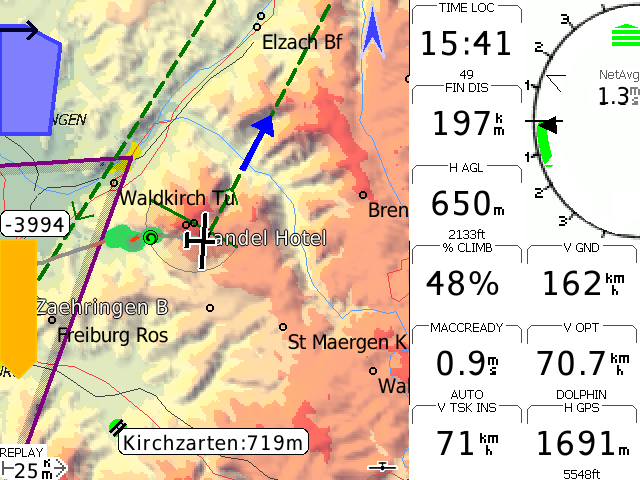
\includegraphics[angle=0,width=\linewidth,keepaspectratio='true']{figures/plain.png}
\caption{Typical XCSoar main screen layout}
\end{figure}

Questo capitolo è una panoramica sui concetti fondamentali dell'interfaccia 
utente di XCSoar. La \emph{schermata principale} copre la maggior parte delle
informazioni necessarie durant eil volo. Tipicamente la schermata principale
è composta dalla mappa mobile e dagli infobox. Per svariati motivi - non 
facenti parte dello scopo di questa introduzione - in volo si può usare una
ampia scelta di schermate principali, dette \emph{pagine}.

Si può accedere facilmente alle pagine con un gesto di scorrimento orizzontale,
proprio come per sfogliare le pagine di un libro, o premendo un pulsante, a 
seconda dell'hardware in uso. 
Con le pagine è possibile comporre svariate schermate principali da usare a
proprio vantaggio in diverse situazioni di volo. In parolepovere, è possibile
accedere facilmente e velocemente alle informazioni appropriate nei diversi
\emph{casi d'uso}. 

Quando in qualche situazione può essere necessario attirare l'attenzione del
pilota, sulla schermata principale può apparire un \emph{overlay}. Questo
succede specialmente se è richiesta una reazione urgente da parte del pilota,
perchè sta per verificarsi una situazione di possibile collisione o di ingresso
in aree di volo con restirizioni.

Evidentemente i pulsanti e le schermate del menu sono overlay anch'essi, e ce
ne sono molti altri. Come risultato, questi elementi messi gli uni sugli altri
formano una pila con la schermata principale alla base. Nei prossimi capitoli
saranno date descrizioni più dettagliate.


\section{Elementi del display}
\subsection*{Schermata principale e pagine}
Ogni pagina dello schermo di XCSoar è composta di diverse parti:
\begin{description}
\item[Area principale] La maggior parte dello chermo è tipicamente dedicata alla
mappa mobile GPS. Su di essa sono sovrapposti svariati simboli relativi alle
informazioni del computer di volo. Lungo il bordo inferiore dello schermo possono
apparire testo ed icone, pe rindicare lo stato dei dispositivi connessi, la
modalità di volo etc.
Con il processo di sviluppo di XCSoar c'è un crescente numero di cose che si può
scegliere di mostrare nell'area principale, come indicatori, radar FLARM, 
assistente di termica e orizzonte.
\item[InfoBox] Una griglia di dati è tipicamente mostrata lungo le parti superiore 
ed inferiore dello schermo (orientamento verticale) o alla destra ed alla sinistra 
(orientamento orizzontale).  Questi cosiddetti InfoBox mostrano i dati provenienti 
dal GPS ed altri dispositivi di input, così come dati calcolati da XCSoar. Inoltre,
gli InfoBox possono mostrare anche indicatori ed alcuni grafici.
\item[Area inferiore] Al fondo dello schermo, XCSoar può disegnare una sezione
trasversale del terreno e dello spazio aereo nella direzione in cui si sta puntando.
\end{description}

\subsection*{Overlay}
\begin{description}
\item[Indicatori]  Gli indicatori rappresentano la strumentazione. Tutti gli indicatori
sono opzionali ed alcuni potrebbero mostrare informazioni significative solo
se XCSoar è connesso ad uno strumento supportato.
Un overlay inidcatore può essere sempre mostrato, o esser einvocato da alcune
condizioni. Per esempio, l'assistente di termcia è mostrato quando XCSoar entra
in modalità Termica. Il radar FLARM è invocato quando viene rilevata una possibile 
collisione.
Indicatori mostrati permanentemente sono, tra gli altri, la barra di planata finale
o la barra del variometro.
\item[Erichette dei pulsanti e menù] Sui dispositivi su cui gira XCSoar, è possibile
utilizzare dei pulsanti hardware per richiamare e navigare piccoli menù sullo schermo,
che sono tipicamente disegnati in modo che le voci siano selezionabili premendo il
pulsante adiacente ad esse.  Se il dispositivo è dotato di touch-screen, le voci del
menù possono essere selezionate toccandole.  Questi pulsanti sono disegnati con testo
nero su sfondo grigio.
\item[Messaggi di stato] Il testo viene mostrato sullo schermo in riquadri di messaggi
di stato.  Questi messaggi vengono utilizzati per mostrare al pilota informazioni 
dettagliate all'occorrere di certi eventi.
\item[Finestre di dialogo] Ampie finestre di dialogo, generalmente contenenti grafici
e pulsanti, sono utilizzate per fornire al pilota dati dettagliati su boe, statistiche,
analisi etc.
\item[Menù principale] Il menù principale è accessibile con un doppio tocco sull'area
della mappa o sugli InfoBox, oppure attraverso un gesto. Se i pulsanti del menù non 
vengono premuti \gesturespec{du} entro un certo tempo, tornano a sparire per non
oscurare l'area della mappa.
\end{description}

\subsection*{Classic vario gauge}
As said above, gauges might be displayed in different ways, either as an 
infobox, overlay, or even in the main area. The traditional variometer gauge is 
different. This needle-style gauge is invoked permanently by choosing an infobox 
layout including the variometer on the right side of the other infoboxes. 

\section{Interaction}
There are several ways to interact with XCSoar:
\begin{itemize}
\item Touching certain map elements
\item Touching InfoBoxes and on-screen menu buttons
\item `Gesturing', by e.g.\ drawing a dash from the left to the right
  on the screen (see Section \ref{sec:gestures} below).
\item `Dragging' the screen (touching the screen and moving before releasing).
\item Pressing application buttons on the device.
\item Pressing the cursor keys on the device.
\item Pressing keys or switches on an instrument connected to XCSoar.
\end{itemize}
Depending on the particular hardware used with XCSoar, not all of these methods
of interaction are possible and there may be different numbers or assignments
of buttons.

For the PC version of XCSoar, clicking the mouse over an item is equivalent to
touching it.

\section{The main button menu}
The button menu is a set of buttons drawn on the screen and activated by touch
or hardware button presses.  Using buttons and the button menu is the primary
way the user interacts with XCSoar.

\subsection*{Interface basics}
The menu is organised into four different groups of functions, usually in
the form of a hierarchy.  The specific menu layout depends on the
hardware button configurations and platform, and may also be customised by the
user.

XCSoar can also accept input from external keyboards, game-pads, joysticks,
stick grip switches etc. A wide variety of functions can be assigned to these
inputs.
\sketch{figures/buttonmenu.png}

On the PC version, these mode buttons are activated by the
1, 2, 3 and 4 keys.  The 6, 7, 8, 9 and 0 keys correspond to the horizontal
strip of buttons.

If the user doesn't interact with the computer for some time, the
menu will close automatically.  This menu time-out is configurable.
The escape key on PC can also be used to close the current menu.

Menu buttons appear greyed out if the corresponding function is not available. 
For example, the ``Waypoint list'' function will appear grey if there are no waypoints loaded.

Several menu button labels have dynamic text based on context, in
order to make it clearer as to what happens when the button is
pressed.  The convention is used that a button's label describes what
will happen when the button is pressed.  For example, if the button
says \bmenug{MC Auto}, then pressing the button will turn on `Auto
MacCready', and the button label will then change to \bmenug{MC Manual}. 
In the menu list described below, generic labels are used.

\subsection*{Menu function groups}
This section describes the default layout of the menu system on all
platforms.  The functions performed by each button are explained more
fully in following chapters.

For the PC version, the keys 1, 2, 3 and 4 activate the 
corresponding menu.  The following menu item list has on the left side of most 
of the menu buttons links to the respective section. Follow them to get to all 
related details.

\section{Menu item overview}

\subsection*{Navigation menu}
\noindent\makebox[\textwidth]{%

\begin{tabularx}{1.44\textwidth}{c|ccccc}
\bmenus{Nav 1/2}
 & \bmenus{Task}
 & \bmenut{Previous}{Turnpoint}
 & \bmenut{Next}{Turnpoint}
 & \bmenut{Waypoint}{List}
 & \bmenus{Alternates} \\
see
 & \ref{cha:tasks}
 & \ref{sec:advanc-rest-tasks}
 & \ref{sec:advanc-rest-tasks}
 & \ref{sec:waypoint-selector-dialog}
 & \ref{sec:alternates} \\ \\
\bmenus{Nav 2/2}
 & \bmenut{Task}{Abort}
 & \bmenut{Mark}{Drop}
 & \bmenus{Target}
 & {}
 & {} \\
see
 & \ref{sec:taskabort}
 & \ref{sec:markers}
 & \ref{sec:waypointdetails}
\end{tabularx}}

You should not start using XCSoar without knowing about the `Alternates' feature. 
Any `Task' related item in the navigation menu is used for planned cross 
country flight and certainly the second step.

\subsection*{Display menu}
\noindent\makebox[\textwidth]{%

\begin{tabularx}{1.44\textwidth}{c|ccccc}
\bmenus{Display 1/2}
 & \bmenut{Zoom}{In}
 & \bmenut{Zoom}{Out}
 & \bmenut{Zoom}{Auto}
 & \bmenut{Info}{Cruise/...}
 & \bmenut{Pan}{On} \\
see
 & \ref{sec:zooming}
 & \ref{sec:zooming}
 & \ref{sec:zooming}
 & \ref{sec:screenpages}
 & \ref{sec:panning} \\ \\
\bmenus{Display 2/2}
 & \bmenut{Labels}{All/...}
 & \bmenut{Trail}{Full/...}
 & \bmenut{Terrain}{On/Off}
 & \bmenut{Topo.}{On/Off}
 & \bmenut{Airspace}{On/Off} \\
see
 & \ref{sec:maplabels}
 & \ref{sec:trail}
 & \ref{sec:terrain_topo}
 & \ref{sec:terrain_topo}
 & \ref{sec:terrain_topo}
\end{tabularx}}

Most of the display menu items are available on gestures, or special key 
short-cuts of your device. Once you are familiar with XCSoar you probably 
will use those menu items less frequently.

\subsection*{Configuration menu}
\noindent\makebox[\textwidth]{%

\begin{tabularx}{1.44\textwidth}{c|ccccc}
\bmenus{Config 1/3}
 & \bmenut{MacCready}{$+$}
 & \bmenut{MacCready}{$-$}
 & \bmenut{MacCready}{Auto}
 & \bmenus{Flight}
 & \bmenus{Wind} \\
see
 & \ref{sec:stf}
 & \ref{sec:stf}
 & \ref{sec:auto-maccready}
 & \ref{sec:flight-setup}
 & \ref{sec:wind-setup} \\ \\
\bmenus{Config 2/3} 
 & \bmenus{System}
 & \bmenus{Plane}
 & \bmenus{Devices}
 & \bmenut{File}{Manager}
 & \bmenus{Replay} \\
see
 & \ref{cha:configuration}
 & \ref{sec:glidepolar}
 & \ref{conf:comdevices}
 & {}
 & \ref{sec:logger-replay} \\ \\
\bmenus{Config 3/3} 
 & \bmenut{Logger}{Start}
 & \bmenus{Raw Logger}
 & \bmenus{Airspace}
 & \bmenus{Vega}
 & \bmenus{Profiles} \\
see
 & \ref{sec:logger}
 & \ref{sec:raw-logger}
 & \ref{sec:airspace-filter}
 & {}
 & {}
\end{tabularx}}

The configuration menu is typically part of the ground interaction with 
XCSoar. You are not expected to spend much time in-flight with tweaking 
the configuration, except you manually adjust wind or MacCready settings. 
The `Vega' item gives control over the  Vega intelligent variometer. This 
comprises a sub-menu.


\subsection*{Information menu}
\noindent\makebox[\textwidth]{%

\begin{tabularx}{1.44\textwidth}{c|ccccc}
\bmenus{Info 1/3}
 & \bmenut{FLARM}{Radar}
 & \bmenut{METAR}{TAF}
 & \bmenut{What's}{here?}
 & \bmenut{Check}{list}
 & \bmenus{Analysis} \\
see
 & \ref{sec:flarm-traffic}
 & \ref{sec:metar-taf}
 & {}
 & \ref{sec:checklist}
 & \ref{sec:analysis-climb} \\ \\
\bmenus{Info 2/3}
 & \bmenus{Status}
 & \bmenus{Weather}
 & \bmenut{Team}{Code}
 & \bmenut{FLARM}{Details}
 & \bmenut{Thermal}{Assistant} \\
see
 & \ref{sec:flight-status}
 & \ref{sec:weather-forecast}
 & \ref{sec:team-flying}
 & {}
 & \ref{sec:thermal-assistant} \\ \\
\bmenus{Info 3/3}
 & \bmenus{Credits}
 & \bmenus{Airspaces}
 & \bmenut{Message}{Repeat}
 & {}
 & {} \\
see
 & \ref{sec:credits}
 & 
 & 
 & 
 &
\end{tabularx}}

The information menu is always a good address, when not only a clue on 
how to set MacCready is requested, but rather more elaborate help on a 
larger scope tactical decision on your flight is requested. %TODO rewrite


\subsection*{The Vega variometer sub-menu of the configuration menu}
\noindent\makebox[\textwidth]{%

\begin{tabularx}{1.44\textwidth}{c|ccccc}
\bmenus{Vega 1}
 & \bmenut{Airframe}{Switches}
 & \bmenut{Setup}{Audio}
 & \bmenut{Manual}{Demo}
 & \bmenut{Setup}{Stall}
 & \bmenus{Accel} \\ \\
\bmenus{Vega 2}
 & \bmenut{ASI}{Zero}
 & \bmenut{Accel}{Zero}
 & \bmenus{Store}
 & \bmenut{Cruise}{Demo}
 & \bmenut{Climb}{Demo}
\end{tabularx}}

The functions in this sub-menu require the Vega intelligent variometer. 
The menu can only be accessed if `Vega' is selected as the connected device.

\subsection*{The pan mode sub-menu of the Display menu}

\noindent\makebox[\textwidth]{%

\begin{tabularx}{1.44\textwidth}{c|ccccc}
\bmenus{Pan}
 & \bmenut{Pan}{Off}
 & \bmenut{Zoom}{in}
 & \bmenut{Zoom}{out}
 & \bmenut{What's}{here?}
 & {} \\
see
 & \ref{sec:panning}
 & {}
 & {}
 & {}
 & {}
\end{tabularx}}

This sub-menu unfortunately overlays the full-screen map view of the pan mode.
 Its functions are quite evident, although the menu could be replaced by multi-touch
 technology or knobs. Besides the essential `exit pan mode'
 function the `What's here?' button offers brilliant access to the variety of
 information of the map.

\section{Default menu buttons}

When no menu is active, (so-called default mode), the horizontal row
of buttons perform the following functions (from left to right):

\begin{center}
\begin{tabular}{c c c c c c}
 PC: & 6 & 7 & 8 & 9 & 0 \\
& \bmenus{Flight} & \bmenut{Task}{Manager} & {} & \bmenus{Target} & \bmenut{Drop}{Mark} \\
\end{tabular}	
\end{center}

For all other versions in the default mode, the cursor keys perform
the following functions:
\begin{jspecs}
\item[Up key] Zoom in
\item[Down key] Zoom out
\item[Left key] Drop marker
\item[Right key] Toggle through normal/aux. InfoBoxes and full-screen
\item[Enter] Clear status message or suppress FLARM gauge if open and no warning
active
\end{jspecs}

\subsection*{Dynamic menu labels}
Certain menu items have dynamic labels to make it clearer what happens when the
menu item is selected.  Furthermore, items that are not available are greyed
out to indicate that selecting the menu item will not do anything.

The convention used for dynamic menu labels is for the labels to display the
action that will be performed once the menu item is selected. For example 
``Lights On'' will turn the lights on, and the menu will be updated to display
``Lights Off'', which would then if pressed turn the lights off. This
convention is used throughout XCSoar.

A selection of key dynamic menu items is presented below:
\begin{description}
\item[\bmenug{Next Turnpoint}]  
  Greyed out if the task is cleared, or if the active turnpoint is the
  finish. If the currently active turnpoint is the turnpoint prior to the 
  finish, this displays  ``Waypoint finish''.
\item[\bmenug{Previous Turnpoint}]  
  Greyed out if the task is cleared, or if the active turnpoint is the
  start and there are no multiple start points.  If there are multiple
  start points and the active turnpoint is the start, then this
  displays ``Cycle start'' to allow selection between the various
  start points.  If the active turnpoint is the first turnpoint after 
  the start, this displays ``Waypoint Start''.
\item[\bmenug{Labels All}]  
  This will turn on all labels available on the map. There are more options to 
  only show a reduced set of labels like ``Labels Task'', thus not cluttering the 
  screen too much.
\item[\bmenug{Target}]  
  Greyed out if the task is cleared or in task abort.
\end{description}


\section{InfoBoxes and screen pages}\label{sec:infoboxandpages}

The information displayed in the InfoBox fields can be selected from a
wide variety of options (listed in Chapter~\ref{cha:infobox}). These
fields can also be used to change for example the MacCready setting.

The specific number and layout of the InfoBox grid depends on the
screen orientation and the device's display size.  

For a 320x240 display
Pocket PC in portrait mode, there are four InfoBoxes above and four
InfoBoxes below the map display.  %TODO Update the example by considering something else than a Pocket PC
\sketch{figures/infoboxes.png}

A typical landscape layout has 9 InfoBoxes and the variometer gauge 
to the right of the map display. 
For larger displays up to 24 InfoBoxes may be displayed simultaneously.  

In order to gain clarity, the less infoboxes you choose to be displayed at once, 
the faster your reading will be. On the other hand, there are much too many 
InfoBox options a pilot would hardly reject. The number of possible InfoBox 
options already exceeded one hundred. That is why XCSoar offers two ways of 
managing even more options than Info\emph{boxes} count.

Depending on your flight's state, whether you are circling or cruising, you can 
let XCSoar change the content of each single InfoBox. As an example you might 
change the display of the actual average climb whilst circling to speed to fly 
when cruising. The switch is derived automatically by entering different 
\emph{flight modes} (see section \ref{sec:flightmodes}) executing a switch to 
another \emph{InfoBox set}.

Further, you can use screen pages to change InfoBox content manually, by 
assigning different Infobox sets to different pages (see following section).

To gain access to automatic switching InfoBoxes dependent on the flight mode, 
just let XCSoar run with its pre-configured setup from installation. To set up 
your personal version of Infoboxes go through the following procedure.
\begin{description}
\item[InfoBox geometry] Choose a basic Infobox geometry or layout.  This basic 
layout is maintained through any changes in-flight, affecting InfoBox content 
only.\config{interface-appearance}
\item[Choose Infobox set ``Auto''] Configure at least one screen page with the
choice of Infoboxes ``Auto''. As can be seen on the corresponding configuration
screen, there are more screen pages pre-defined. \config{screenpages}  These 
others are not needed to gain automatic switches by flight mode. They are for \emph{manually} turning through the screens defined by pages. 
\item[Define InfoBox sets] Put together the Infobox content you want to be 
displayed in three Infobox sets called ``Circling'', ``Cruise'', and ``FinalGlide''
respectively.\config{infobox_sets}
\end{description}  


\subsection*{Screen pages with different InfoBox sets}\label{sec:screenpages}

XCSoar allows the pilot to define various sets of InfoBoxes that are 
appropriate for ``normal'' states of flight.  Assuming circling,
cruising, or final glide as normal, XCSoar can switch corresponding Infobox 
sets automatically.

As you might imagine, there are countless cases, you wished you had another 
ensemble of information displayed at once.  For all of these more or less 
special situations you can define up to eight screen pages, reflecting the 
actual \emph{use case}. Just to draw a brief sketch of the possibilities 
introduced by the concept of screen pages, a few use cases are given. 
\label{par:use_case}
\begin{description}
\item[Familiarisation] Especially if you are a beginner, you might study 
computed values in-flight in advance of placing them in your ``normal'' InfoBox
ensemble - just to get familiar with the reading. To do so, create a new 
Infobox named ``test'' to be placed on an additional screen page brought in. In
any case you can go back to the screen you know by ``turning a page''
\item[Competition] If you are a pilot scratching the edge, you might want to 
gain benefit of XCSoar's numerous task- and competition-related computations. 
In order to get them related to the competition's phases, you might like the 
idea of defining two special use cases with pages for the phase before start, 
another one for whilst racing.  If you are in search of a specific value to
be displayed, give it a try in chapter \ref{cha:infobox} ``\nameref{cha:infobox}''.
There is a big chance you will find it.
\item[On the ground] As a manager on duty you might use a screen page, showing 
the ``FLARM Radar'' solely.  This might happen on a PC screen running XCSoar
being connected to a FLARM receiver.
\end{description}

Whatever you would like to display, take into account the use case and screen 
pages concept.

\gesturespec{left}
To go through the various screen pages, use gesture left/right (touch-screen), or via menu button in menu \bmenug{Display 1/2}, showing a dynamic label, changing accordingly to the screenpage's content to show up next:
\gesturespec{right}

\bmenut{Display}{1/2}\blink\bmenut{Info}{Circling}\blink\bmenut{Info}{Cruise}\blink\bmenut{Info}{FinalGlide}\blink\bmenut{Info}{...}


\subsection*{Modifying InfoBox content}

(This section applies only when a touch-screen or mouse is present.)

Some InfoBox values can be changed by the user by selecting (i.e.\ long-pressing) the
InfoBox with the touch-screen or mouse.  This brings up a small tabular dialogue:

\begin{description}
\item[\bmenuw{Edit}]  
  Allows the pilot to adjust the InfoBox setting (e.g.\ raise or lower the
  MacCready setting)

\item[\bmenuw{Setup}]
  Allows you to change the behaviour of the setting related to the InfoBox 
  (for example, changing from auto to manual MacCready mode); or 
  to change the InfoBox itself by pressing `\emph{Switch InfoBox}', then 
  choosing from a list of all available InfoBoxes.

\end{description}

Examples of InfoBoxes that can
be adjusted include MacCready setting, wind speed, and altitude (QNH).


\subsection*{Changing InfoBox sets}

An entire set of InfoBox can be composed by the `\emph{Setup System}' configuration 
dialogues on the `\emph{Look / InfoBox Modes}' and `\emph{Look / InfoBox Pages}' 
\ref{sec:infobox_sets} setup page. 
The dialogues give a wide variety to set up the look and feel of the XCSoar pages.  


\section{Status messages}

Status messages appear over the map area to present text for a short period of
time.  The message disappears after the time period has elapsed, and different
types of message have different periods. Additionally, status messages can be
made to disappear by acknowledging the message.  Acknowledgement is achieved by
either pressing the enter key, touching the status
message (on touch-screen devices) or clicking the screen (mouse enabled devices).

Additional user buttons may be assigned to a status message repeat function,
which brings up the last message again.
\sketch{figures/status-message.png}

Typical status messages include:
\begin{itemize}
\item Airspace queries
\item Airspace warnings
\item User interface events (e.g.\ changing display modes)
\item Glide computer events (e.g.\ take-off, turning waypoints)
\end{itemize}

Note that status messages do not appear while a dialogue is on screen, the
messages are buffered and displayed as soon as the dialogue is exited.


\section{Dialogue windows}\label{sec:dialog-windows}

XCSoar contains several dialogue windows that can be activated to bring up
additional information and are also used for more complex interactions with the
user, such as editing tasks and configuring settings.

Some dialogues simply display information, and require no user input. Other
dialogues contain data fields that can be modified or buttons that can be pressed.  

A cursor appears over the active button or data field. Pressing the up/down
arrow keys, the cursor will cycle
through the next or previous items. For list items and scrollable text, the
up/down arrow key moves the cursor up or down the list or text, and the
left/right arrow keys move the cursor up or down by one page in long lists.

For PDAs and PC versions, list items can be selected by touching the item (or
left-clicking with the mouse). Once a list item is selected, another touch
(left click) is equivalent to pressing the enter key.

Pressing the right/left arrow keys, the data field value under the
cursor can be modified. Pressing the enter key activates the button or
makes a selection from a list.

Dialogues are typically started from the button menu.  

Many of the dialogue windows have multiple pages of information and are controlled
in a consistent fashion. Press the \bmenuw{$<$} or \bmenuw{$>$} buttons to
select the next or previous page of the dialogue and the \bmenuw{Close} button 
to make the dialogue disappear.

The escape key on a PC can also be used to close dialogues.

The user must close the dialogue to return to the map view. When a dialogue
has been opened, the main button menu is disabled until the dialogue is closed.

In some dialogues, items that are not relevant or valid (such as AAT details when
flying a non-AAT task) are not displayed.

A summary of the major dialogues is presented below.
\begin{description}
\item[Flight setup] Used to modify the polar of the glider both before and
during flight, as well as to set the QNH pressure
\item[Wind] Used to modify or adjust the estimated wind magnitude and direction
\item[Waypoint details] Describes a waypoint in detail and has navigation
functions such as `GoTo' and `Insert in Task'
\item[Waypoint list] Used to select a waypoint from the waypoint database
\item[Task manager] Used to create, modify and view cross country tasks
\item[Analysis] Shows several pages of analysis and statistics about the flight
\item[Status] The status dialogues give summaries of the situation of the 
aircraft, system, task, start and times
\item[Configuration] Allows XCSoar and certain connected devices to be
configured
\item[Airspace filter] Controls enabling and disabling the display and warnings
of each airspace class
\item[Team code] Allows transfer of coordinates between FLARM team mates via a 
  code
\item[Devices]  Selection of various external devices (e.g.\ smart variometers,
  FLARM, etc.).
\item[Setup Plane]  Easy reconfiguration of the plane-dependent settings (e.g. 
  polar, competition ID, etc.) by choosing from a list of previously-created 
  plane profiles.
\end{description}

These dialogues are described in later chapters, with the exception of the
check-list, status and text entry dialogues, which are described below.


\subsection*{Check-list (dialogue example)}\label{sec:checklist}

The checklist dialogue can display several pages of user-defined free text.
Typically this is used for check-lists. It can be accessed via the menu.

\bmenut{Info}{1/3}\blink\bmenut{Check}{List}
\sketch{figures/checklist.png}

These check-lists may include: daily inspection, preflight,
out-landing, pre-landing, radio procedures, and aircraft rigging and
de-rigging instructions.  Since the check-lists may be long, the
up/down keys may be used to scroll through the text. Clicking the
\bmenuw{$<$} and \bmenuw{$>$} buttons selects the previous/next
checklist.


\subsection*{Text entry} \label{sec:textentry}

A text entry dialogue is used for entering text.  This is used for team
code entry, setting file names, waypoint editing, as well as entering
other configuration options, such as pilot name for the logger.

Two ways of entering text are provided. 

To enter text in `high score style', use the A+/A- buttons to adjust the 
\sketch{figures/textentry.png}
character under the cursor (underlined character). Clicking the \button{$<$} 
and \button{$>$} buttons move the cursor left/right.  

To enter text with the touch screen keyboard, press the letters of choice 
one after the other. In some dialogues (e.g.\ waypoint editing) only the next
\sketch{figures/textentry_keyboard.png}
letters matching to an entry in the database will be shown. For deleting the 
last letter use the \button{$<-$} button. The \button{Clear} button deletes all input.

Press \button{Ok} to validate, or \button{Cancel} to exit.


\section{Acoustic alert and sound feedback}

XCSoar generates sounds for different events, and can be configured to
have custom sounds for any event.  See Section~\ref{sec:status-file} for
details on customisation.

When XCSoar is connected to the Vega intelligent variometer, it sends
commands to Vega's speech system, to give verbal clues and warnings such as:
\begin{itemize}
\item Final glide through terrain
\item Approaching/passing a task waypoint
\item Airspace warnings
\end{itemize}

The XCSoar user interface also can connect sound feedback to the completion 
of any command like:
\begin{itemize}
\item Marker dropped
\end{itemize}


\section{Screen visuals}

Certain aspects of the look of items on the screen can be adjusted.
The most noticeable of these is whether to display InfoBoxes and
gauges in white on black (called inverse colours) or black on white.


\section{Help system}

A help system provides descriptive text for properties in most
dialogues.

\section{Interfacing with gestures}\label{sec:gestures}
As of version 6.0, XCSoar supports so-called `gestures'.

To use this feature hold down the finger on the 
touch-screen (or mouse button at the PC), draw a certain figure and release 
the touch-screen / mouse button. Depending on the figure that was drawn 
a certain function is activated. \sketch{figures/gesture1.png}

A specific gesture is defined by movements of the finger or the 
cursor in the four directions Up, Down, Left and Right. This means if 
you drag your finger down and afterwards to the right over the screen, 
\gesture{dr} the gesture ``DR'' is detected, which stands for ``Down-Right''.
It will bring up the waypoint list. The manual indicates an available 
gesture as shown here on the left side of the text body. Both the blue hand 
and pictogram of the movement are used to indicate a specific gesture, in this 
case move down then to the right. A list of generally available gestures is 
shown below. \gesturespec{dr}
\vspace{2em}

\subsection*{Most common or basic gestures:}
\begin{itemize}
\item[\raisebox{-1em}
{
\includegraphics[angle=0,width=0.1\linewidth,keepaspectratio='true']{figures/du.png}}] DU, denoting a check mark: Show main menu 
\item[\raisebox{-1em}
{
\includegraphics[angle=0,width=0.1\linewidth,keepaspectratio='true']{figures/up.png}}] U: Zoom in 
\item[\raisebox{-1em}
{
\includegraphics[angle=0,width=0.1\linewidth,keepaspectratio='true']{figures/down.png}}] D: Zoom out 
\item[\raisebox{-1em}
{
\includegraphics[angle=0,width=0.1\linewidth,keepaspectratio='true']{figures/left.png}}] L: Turn screen page pro-grade (Normal, Aux., Full-screen...) 
\item[\raisebox{-1em}
{
\includegraphics[angle=0,width=0.1\linewidth,keepaspectratio='true']{figures/right.png}}] R: Turn screen page retrograde (Normal, Full-screen...) 
\item[\raisebox{-1em}
{
\includegraphics[angle=0,width=0.1\linewidth,keepaspectratio='true']{figures/urdl.png}}] URDL, denoting a P: \textbf{P}an-mode. Might also be invoked by 
moving two fingers apart on the screen.
\end{itemize}
\vspace{2em}

\subsection*{More gestures available:}
\begin{itemize}
\item[\raisebox{-1em}
{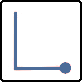
\includegraphics[angle=0,width=0.1\linewidth,keepaspectratio='true']{figures/dr.png}}] DR, denoting an L: Show the Select Waypoint dialogue similar to menu 
item Waypoint \textbf{L}ist
\item[\raisebox{-1em}
{
\includegraphics[angle=0,width=0.1\linewidth,keepaspectratio='true']{figures/rd.png}}] RD, denoting a T: opens the \textbf{T}ask Manager
\item[\raisebox{-1em}
{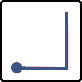
\includegraphics[angle=0,width=0.1\linewidth,keepaspectratio='true']{figures/dl.png}}] DL: show the Alternates List
\item[\raisebox{-1em}
{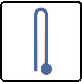
\includegraphics[angle=0,width=0.1\linewidth,keepaspectratio='true']{figures/ud.png}}] UD: enables Auto-Zoom
\end{itemize}
\vspace{2em}

\subsection*{Sophisticated dialogues:}
\begin{itemize}
\item[\raisebox{-1em}
{
\includegraphics[angle=0,width=0.1\linewidth,keepaspectratio='true']{figures/urd.png}}] URD, denoting an A: Show the \textbf{A}nalysis dialogue.
\item[\raisebox{-1em}
{
\includegraphics[angle=0,width=0.1\linewidth,keepaspectratio='true']{figures/ldrdl.png}}] LDRDL, denoting an S: Open the \textbf{S}tatus dialogue
\end{itemize}


%%%%%%%%%%%%%%%%%%%%%%
\chapter{Navigation}\label{cha:navigation}
This chapter describes the moving map display as an aid to navigation,
and also describes some of the task and glide related overlays on the
map display.

\section{Map display elements}

\begin{maxipage}
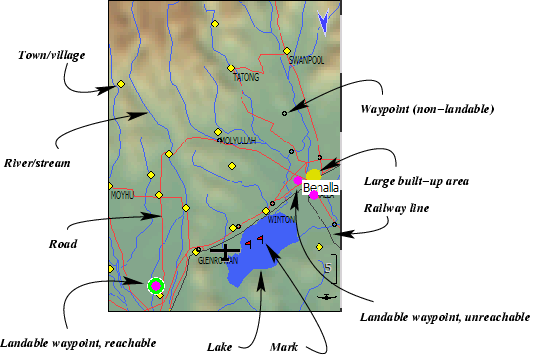
\includegraphics[angle=0,width=0.9\linewidth,keepaspectratio='true']{figures/fig-map.png}
\end{maxipage}

The moving map shows:
\begin{enumerate} 
\item Glider, wind indicator, thermal profile, final glide indicator
\item Terrain, relief and hight of the terrain
\item Topography, rivers, roads, towns
\item Waypoints, airports, landables
\item The active task, observation zones, turnpoints
\item The bearing (or route\footnote{The line to the next waypoint may be a 
  \emph{route}, as described in Section~\ref{sec:route}.}) to the next waypoint, 
  heading
\item Airspaces
\item Markers, thermals history, snail trail
\item Glide range\footnote{The glide range is also referred to as the 
  \emph{reach}, as described in Section~\ref{sec:reach}.}
\end{enumerate}
The map is drawn in a projected coordinate system (not latitude and
longitude), and the scale can be changed (zooming in and out), as well
as panned.  All navigation functions take the curvature of the Earth
into account.

\section{Glider symbol, map orientation}
The glider symbol shows the position of the glider on the map.  The
orientation of the glider indicates the estimated heading of the
glider.

The map is oriented in one of three ways: North up,
Track up, or Target up.  Configuration settings \config{orientation} can be used
to specify a different map orientation when in circling mode. This is useful to prevent
disorientation when looking at the map while circling.  Target-up when
circling makes it easy to determine which direction to exit the
thermal.

When Track or Target-up is used in circling mode, the glider symbol is
centred on the screen, even if the symbol position is configured differently.
In cruise mode the Track and the Target-up orientation allows the glider
symbol to be positioned (e.g.) 20\% from the bottom of the screen, giving a good view of the
map ahead of the glider.  This position is adjustable in the configuration
\config{gliderposition} settings.

\section{Zoom and map scale}\label{sec:zooming}

To change the scale of the map, depending on the hardware you use:
\begin{enumerate}
\item Tap/click on a blank part of the map to highlight the map if it is not
already selected.
Then use mouse wheel, or the Pocket PC up/down key to either zoom
in or out.
\item Android devices have the +/- rocker that let you change the zoom (it usually allows for adjusting the sound volume). It may be difficult to access during a flight, when the device in on a generic mount.
\item You can also gesture to change the zoom level. Gesture 
Up (see left) zooms in, Down zooms out.\gesturespec{up}
\item Or select the function from the menu.
\begin{quote}
\bmenug{Display 1}\blink\bmenug{Zoom In} and \bmenug{Zoom Out}
\end{quote}
\end{enumerate}

The map scale is displayed in the lower left corner of the moving map
display. The indicated distance is measured from the left to the right border
of the map display.
\marginpar{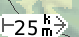
\includegraphics[angle=0,width=0.4\linewidth,keepaspectratio='true']{figures/zoom.png}}

Compaq Aero Users. If you enable the Compaq Aero Game Keys (On the
Q-menu) the centre two front buttons become the up/down keys.

\subsection*{Circling Zoom}
There is a facility to have two zoom settings; one when the glider is
in circling mode, and one in the cruise or final mode.  This is the `\emph{Circling zoom}' 
option in the \config{circlingzoom} configuration settings.  
By default, the circling zoom is set to about 2.5 km - 5.0 km, depending on the
display size. When the user zooms in or out, it affects the current
mode's zoom setting only, so when leaving the mode the previous mode's
zoom setting is used.  If `\emph{Circling Zoom}' is not enabled,
there is only a single zoom level.
This leads to different zoom levels being preserved to be managed manually, 
independent of the following Auto Zoom settings.

\subsection*{Auto Zoom}
Auto Zoom automatically zooms in when approaching a waypoint to keep
the waypoint at a reasonable screen distance. When \emph{Auto Zoom} is active,
`AUTO' appears next to the map scale.
\marginpar{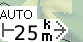
\includegraphics[angle=0,width=0.4\linewidth,keepaspectratio='true']{figures/zoomauto.png}}

To invoke Auto Zoom use the gesture \gesturespec{ud}
or menu path depicted to the left. 
Switching back to manual zoom is simply done by using the same menu path
or just zooming manually, no matter whether done via menu or gesture.
\menulabel{\bmenug{Display 1}\blink\bmenut{Zoom}{Auto}}

When a waypoint changes (automatically, via the task selector, or by
manually switching waypoints), \emph{Auto Zoom} adjusts the zoom level
automatically so that the next waypoint is visible on the map.

During circling, if a thermal has been detected, then the map is centred about
the thermal or part-way such that the glider is still visible.

\section{Panning the map}\label{sec:panning}

A pan mode allows the user to explore areas beyond the glider.  This
is particularly useful when task planning.
\begin{enumerate}
\menulabel{\bmenug{Display 1}\blink\bmenug{Pan On}}
\item Enable pan mode by button menu or by gesture.  The gesture for this is moving your fingertip up, right, down, left, supposed to form a ``P''.
\gesturespec{urdl}
\item The map can then be panned by dragging the screen or using the cursor
  keys.
\item When done, pan mode has to be disabled manually, by pressing `\emph{Pan Off}' 
  from the special sub-menu of buttons in pan mode.
\end{enumerate} 

\sketch{figures/pan.png}
When pan is active, the letters `PAN' appears next to the map scale.  While
panning the location of the focus stays in the middle of the display under the
cross hairs. 

Despite the focus under the cross-hairs the map
still offers the `\emph{What's here?}' feature just by touching any 
position on the map (presuming a touch-screen).


\section{Waypoints}\label{sec:waypoint-schemes}
Waypoints are displayed with different symbols depending on the
waypoint type; the major distinction being landable and non-landable
waypoints.

\subsection*{Landables}
The waypoint symbols are drawn as shown below. There are three icon sets for
landable waypoints. \config{waypointicons}

\begin{tabular}{c|ccc|ccc|}
Icon set 
&\begin{sideways}Landable field\end{sideways}
&\begin{sideways}Marginal\end{sideways}
&\begin{sideways}Reachable\end{sideways}
&\begin{sideways}Airfield\end{sideways}
&\begin{sideways}Marginal\end{sideways}
&\begin{sideways}Reachable\end{sideways}\\
\hline
Purple Circle &
\includegraphics[width=0.8cm]{icons/winpilot_landable.pdf} &
\includegraphics[width=0.8cm]{icons/winpilot_marginal.pdf} &
\includegraphics[width=0.8cm]{icons/winpilot_reachable.pdf} &
\colorbox{white}{\includegraphics[width=0.8cm]{icons/winpilot_landable.pdf}} &
\includegraphics[width=0.8cm]{icons/winpilot_marginal.pdf} &
\includegraphics[width=0.8cm]{icons/winpilot_reachable.pdf} \\
\hline
B/W & 
\includegraphics[width=0.9cm]{icons/alt_landable_field.pdf} &
\includegraphics[width=0.9cm]{icons/alt_marginal_field.pdf} &
\includegraphics[width=0.9cm]{icons/alt_reachable_field.pdf} &
\colorbox[rgb]{0.94,0.94,0.94}{\includegraphics[width=0.9cm]{icons/alt_landable_airport.pdf}} &
\includegraphics[width=0.9cm]{icons/alt_marginal_airport.pdf} &
\includegraphics[width=0.9cm]{icons/alt_reachable_airport.pdf} \\
\hline
Traffic lights & 
\includegraphics[width=0.9cm]{icons/alt2_landable_field.pdf} &
\includegraphics[width=0.9cm]{icons/alt2_marginal_field.pdf} &
\includegraphics[width=0.9cm]{icons/alt_reachable_field.pdf} &
\colorbox{white}{\includegraphics[width=0.9cm]{icons/alt2_landable_airport.pdf}} &
\includegraphics[width=0.9cm]{icons/alt2_marginal_airport.pdf} &
\includegraphics[width=0.9cm]{icons/alt_reachable_airport.pdf} \\
\hline
\end{tabular}

The \emph{marginal} icons are drawn for those waypoints which are principally in the 
reach, but it is not possible to approach them directly. E.g.\ a mountain prohibits a direct approach.
  
Waypoints are optionally labelled according to one of several
abbreviation schemes \config{labels} and visibility.

On top of this landable waypoints can be displayed in more detail. If
`\emph{Detailed landables}' is switched on you get additional information
encoded in the appearance of it's icon. 
\begin{enumerate}
\item  Landable fields get a square-shaped icon despite what is shown in the table.
  The square is drawn like a diamond standing on one corner. Airfields stay with the 
  circle shape, so that they become easy to distinguish.
\item  All icon sets, including the `Purple Circle' icon set, get the 
  runway turned into their actual direction. The runway direction has to be available in 
  the waypoint data. E.g.\ the SeeYou waypoint file format (\verb|.cup|) does
  include this information.  
\end{enumerate}

\subsection*{Landables in Reach}
Next to landables an estimated arrival height
\emph{above the arrival safety height of reachable landable} points is
displayed next to the waypoint. This feature is one of the most powerful out 
of XCSoar's capabilities. The arrival height is calculated highly 
configurable by XCSoar's \emph{glide computer} with parameters taken into 
account being glider performance (polar), MacCready setting, wind, terrain 
clearance, and --- obviously --- safety heights' values.
With all of it being 
configurable, there is enough room for failure, so please:
Unless you will have fully understood the glide computer's concepts, you 
\warning
better stay with XCSoar's pre-configuration (and in no way judge readings as 
heavenly approved).
It is up to the pilot to always interpret readings and watch values trending 
over time.

However, having set up the glide computer following
Chapter~\ref{cha:glide} the \emph{display} of estimated reach heights, drawn beside 
landables in reach may take into account terrain or not or display both.
\config{arrivalheight}

Another option is to display the required glide ratio next to a landable in 
reach. This calculation is simply derived by the glider's actual distance to 
landables divided by the height difference between actual altitude and 
landable's altitude.  Again, the safety height is added to the landable's 
height, but nothing else taken into account: no wind, no polar, no MacCready 
settings, just geometry. The concept of required glide ratios is a widely 
discussed concept, said as to be a very robust one.

\tip Keep in mind a strong relationship of displays of \emph{reach} and 
settings in the glide computer.

\subsection*{Non-Landables}
As far as your waypoint file contains information on the nature of the 
non-landable waypoints, the map will then display specific icons accordingly. 
Figure~\ref{fig:nonlandables} contains a collection of the currently supported map icons.

\begin{figure}[htbp]
\centering
\vspace{2.5cm}
\begin{tabular}{ccccccccc}
\begin{rotate}{60}Simple waypoint\end{rotate} &
\begin{rotate}{60}Mountain top\end{rotate} &
\begin{rotate}{60}Obstacle\end{rotate} &
\begin{rotate}{60}Pass\end{rotate} &
\begin{rotate}{60}Power plant\end{rotate} &
\begin{rotate}{60}Tower or building\end{rotate} &
\begin{rotate}{60}Tunnel\end{rotate} &
\begin{rotate}{60}Weather station\end{rotate} &
\begin{rotate}{60}Bridge\end{rotate}\\

\includegraphics[width=0.5cm]{icons/map_turnpoint.pdf} &
\includegraphics[width=0.8cm]{icons/map_mountain_top.pdf} &
\includegraphics[width=0.7cm]{icons/map_obstacle.pdf} &
\includegraphics[width=0.7cm]{icons/map_pass.pdf} &
\includegraphics[width=0.8cm]{icons/map_power_plant.pdf} &
\includegraphics[width=0.7cm]{icons/map_tower.pdf} &
\includegraphics[width=0.6cm]{icons/map_tunnel.pdf} &
\includegraphics[width=0.6cm]{icons/map_weather_station.pdf} &
\includegraphics[width=0.8cm]{icons/map_bridge.pdf}
\end{tabular}
\caption{non-landables}\label{fig:nonlandables}
\end{figure}

\section{Active task}

The active task course is drawn on the map as a blue (dashed) line.

Assigned area tasks also show the turn point sectors or areas as a yellow shaded
region.  Circles are always drawn around start and finish points, lines are
only drawn if the start/finish points are of line type.  
Task observation sectors are drawn as circle segments.

At all times a thick black line is drawn from the glider to the next
waypoint in the task.  This line may be the direct path to the waypoint,
or may be a \emph{route} path clearing terrain and airspace obstacles, described in
further detail in Section~\ref{sec:route}.

\begin{center}
\begin{tabular}{c c c}
\emph{Start/finish} & \emph{Sector} & \emph{Cylinder} \\
\includegraphics[angle=0,width=0.3\linewidth,keepaspectratio='true']{figures/cut-startfinish.png} &
\includegraphics[angle=0,width=0.3\linewidth,keepaspectratio='true']{figures/cut-sector.png} &
\includegraphics[angle=0,width=0.3\linewidth,keepaspectratio='true']{figures/cut-barrel.png}
\end{tabular}
\end{center}


\section{Terrain and Topography}\label{sec:terrain_topo}

The following topographical features are drawn on the map:
\begin{itemize}
\item Major roads, shown as red lines
\item Rivers, shown as blue lines
\item Large water bodies (lakes), shown as blue areas
\item Large cities, shown as yellow areas
\item Small population areas, shown as yellow diamonds
\end{itemize}
Cities and small population areas are labeled in italics.

Terrain is coloured according to elevation, and optionally shaded by sun, or 
wind direction.  Invalid terrain, or terrain below
sea level is coloured blue.

\menulabel{\bmenug{Display 2}\blink\bmenut{Terrain}{On/Off}}
\menulabel{\vspace{1cm}\bmenug{Display 2}\blink\bmenut{Topo.}{On/Off}}

Terrain is shaded to improve visibility.  The default shading
is set up so that the virtual lighting position is the wind bearing,
thus brighter areas are on the upwind side of hills and dark areas in
the lee of the hill.  
Support for a sun ephemeris is also implemented. If the slope shading is set 
to `Sun', the brightness of a slope follows the day time in a very natural way.
The amount of shading and overall terrain brightness is configurable. \config{shading}

Both terrain and topography display can be switched on or off from the
menu.

\begin{center}
\begin{tabular}{c c}
Topography & Terrain \\
\includegraphics[angle=0,width=0.4\linewidth,keepaspectratio='true']{figures/cut-topo.png} &
\includegraphics[angle=0,width=0.4\linewidth,keepaspectratio='true']{figures/cut-terrain.png}
\end{tabular}
\end{center}

If the terrain data is not available (or terrain display is turned
off), the background colour of the map window is white.  All terrain
below mean sea level is coloured blue.  If you are flying outside the
terrain region, the background colour will be white.

\subsection*{Map labels}\label{sec:maplabels}

The screen can be de-cluttered, turning off the display of all waypoint labels by toggling the `\emph{Labels}' menu.
\menulabel{\bmenug{Display 2}\blink\bmenut{Labels}{None}}

Other options for display decluttering include:

\jindent{\bmenuth{Labels}{Task \&}{Airfields}}{ Shows labels for the waypoints in 
  the active task and any airfields (based on the waypoint attributes in 
  the waypoints file).  Other waypoints are shown but not labeled. }
\jindent{\bmenut{Labels}{All}}{ Shows labels for all waypoints. }
\jindent{\bmenuth{Labels}{Task \&}{Landables}}{  Shows labels for the waypoints in 
  the active task and any landable fields (based on the waypoint attributes in 
  the waypoints file).  Other waypoints are shown but not labeled. }
\jindent{\bmenut{Labels}{Task}}{ Shows labels only for waypoints in the active task}

Note that in all cases, the label format is configurable in the 
`\emph{Waypoint Display}' configuration menu.  \config{labels}


\section{Trail}\label{sec:trail}

An optional `snail trail' is drawn on the map showing the glider's
path history.  The colour and thickness of the trail depends on the altitude or
on the variometer value. 

\begin{center}
\includegraphics[angle=0,width=0.5\linewidth,keepaspectratio='true']{figures/snail.pdf}
\end{center}

If Vega or an intelligent variometer is connected with Netto output,
the Netto vario value is used; hence the colours and thickness of the
trail indicates the air-mass vertical movement rather than the glider's
vertical movement.

\config{snailtrail}
The snail trail display can be toggled between \emph{Off}, a \emph{Short} trail
(about ten minutes), a \emph{Long} trail (about one hour) or a \emph{Full} trail
which displays the entire flight.  This can be performed permanently
through the configuration settings or temporarily by the
menu.
\menulabel{\bmenug{Display 2}\blink\bmenut{Trail}{Full}}

Note that for all of these modes, the snail trail is short in
circling mode in order to reduce screen clutter.

In order to assist centring thermals in the presence of wind, the
snail trail can be artificially drifted with the wind as it is
displayed (this is drift compensation).  In this way, the snail trail
is referenced to the prevailing wind rather than referenced to the
ground.  Since thermals drift with the wind also, the drifted trails
give a better indication of where the glider has been relative to the
thermals.

An example of this is illustrated below.  Note that when trail drift
compensation is active (right picture), the glider appears to be
circling in a column rather than an elongated spiral (left picture).

\begin{center}
\includegraphics[angle=0,width=0.6\linewidth,keepaspectratio='true']{figures/traildrift.png}
\end{center}

\config{traildrift}
Enabling trail drift compensation is performed through the
configuration settings.  The compensation is only performed
whilst in circling mode; the display of the trail in cruise mode is unaffected.
This can also be performed from the wind settings dialogue.
\menulabel{\bmenug{Config 1}\blink\bmenus{Wind}}

The trail drift display is useful also to show more clearly when thermals
are cranked due to wind shear.

The trail width can optionally be scaled according to the variometer display\config{trailscaled}.


\section{Markers}\label{sec:markers}

Markers are shown as small flags (a) on the map.  The markers can be dropped
manually, by pressing a button, or automatically.  An example use of
automatic markers is to drop markers when entering circling mode, as a
simple way of showing all thermals encountered.

\menulabel{\bmenug{Nav 2}\blink\bmenut{Mark}{Drop}}
Markers are not preserved after XCSoar is exited, however the location
of all marks are appended to the file \verb|xcsoar-marks.txt|.

\section{Thermals}

While climbing in thermals, a marker is automatically generated showing the
thermal location on screen.    The positions of the last 20 thermals are
stored until the end of the flight.
\sketch{figures/thermalhistory.png}
This thermal history is accessible through the map
element functions in the same way as markers or waypoints.


\section{Glide range line}\label{sec:reach}

A reachable glide `footprint' is displayed on the map display as a
black and white dashed line, indicating where the glider would descend
through the terrain clearance height.  The reach shows clearance
tracks extending in all directions, optionally including paths around
terrain obstructions.  This feature is useful in assessing range with
respect to topography when searching low for lift, and when flying in
mountainous areas.

Reach calculations may be configured \config{turningreach} to two levels of detail:
\begin{description}
\item[Straight line] If turning reach is disabled, then the reach shows the
 furthest distance the glider can fly in final glide in all directions without
 turning.  This reach appears as a closed ring around the glider.

\begin{center}
\includegraphics[angle=0,width=0.8\linewidth,keepaspectratio='true']{figures/reach1.png}
% CUTOUT SHOWING GLIDE RANGE FOOTPRINT.  NO TOPOGRAPHY, FULLSCREEN, NO TASK. TURNING=FALSE
\end{center}

\item[Turning] If turning reach is enabled, then the reach shows the
  greatest area the glider can reach in all directions, even allowing
  turns around obstructions.\footnote{The maximum number of turns is
    set to three, and no turns may be greater than 90 degrees.}  The
  reach area appears as a closed ring around the glider but may also
  include holes indicating mountain peaks that the glider cannot reach
  without further climb.

\begin{center}
\includegraphics[angle=0,width=0.8\linewidth,keepaspectratio='true']{figures/reach2.png}
% CUTOUT SHOWING GLIDE RANGE FOOTPRINT.  NO TOPOGRAPHY, FULLSCREEN, NO TASK. TURNING=TRUE
\end{center}

\end{description}

The display can be configured to additionally blur the unreachable area
outside the glide range. \config{gliderange}
The final glide path is checked for whether the glider clears terrain along
the path by the terrain clearance height (see Section~\ref{sec:safety-heights}).
If clearance is not attained, a red
cross appears on the map at the point where the violation occurs. If a target is
defined the calculation is done along the straight path to the target. If no 
target is defined the calculation is done along the current heading.

If reach is enabled, then the reachability of landable waypoints is used
by the abort task mode, alternate landable option lists and display of
landable waypoints on the map.

Note that task calculations are otherwise unaffected by reach
calculations --- for example, altitudes required as shown in the final
glide bar or task data as displayed in infoboxes do not take reach into account.

Furthermore, the reach calculations are used for footprint, landable
waypoint arrival heights, abort mode and the alternates dialogue.  The glider
performance and MacCready setting used in these calculations are configurable\config{reachpolar}:
\begin{description}
\item[Task] The MC value is that used in the task.
\item[Safety MC] A configurable, typically low MC value is set by the user to set
  performance near, but slightly degraded, to best glide performance. The amount of safety 
  in the reach calculation is then the gap between best glide performance and the glide
  performance following the safety MC speed to fly. 
\end{description}

\section{Status tabs `\emph{Flight}' and `\emph{Time}'}\label{sec:flight-status}

The status dialogue is a multi-tabular dialogue giving overview information on the 
flight, system, task, rules and times.
These are information, and hence cannot be modified by the user.
It is accessed via the gesture ``S'', or with the button menu.
\gesture{Left - Down - Right - Down - Left}
\begin{quote}
\bmenug{Info 2}\blink\bmenug{Status}
\end{quote}

\subsection*{Flight}
Select the tabular page `\emph{Flight}'. 
The flight status dialogue shows the status of the aircraft's locality.
It shows the location of the aircraft, the
maximum height gain, and nearest waypoint it's bearing and distance.
\sketch{figures/status-flight.png}

You may find this function useful when you need to report your
location to others.

\subsection*{Times}\label{sec:time-status}
Select the tabular page `\emph{Times}'. 
It shows the local time, UTC time and date, flight duration, takeoff and landing time, and
the local sunrise and sunset times.

Note that the values in the Status dialogue 
are static once the particular dialogue page is displayed. 
\sketch{figures/status-times.png}
That is, position, times, etc.\ do not update while the page is displayed.
To see the updated values, it is necessary to select a different tabular, 
then return to the previous dialogue to see the new values.


\section{Route}\label{sec:route}

XCSoar can plan paths around terrain and airspace obstacles in three
dimensions from the aircraft to the destination.  Such a path is known
as a route.  The height of the destination is the arrival height for
final waypoints, or may be higher for intermediate waypoints, as
dictated by the task system as required to complete the task.  Route
planning functions in normal ordered task mode, abort mode and goto
mode.

\begin{center}
\includegraphics[angle=0,width=0.8\linewidth,keepaspectratio='true']{figures/route3.png}
\end{center}

Routes take into account the glider polar performance and are
calculated to be optimal in the sense of minimum time.  By default,
route calculation is disabled, and can be enabled for terrain only or
terrain and airspace avoidance. \config{routemode}

Terrain is avoided vertically by the terrain safety height,\config{safetyterrain}
with no additional lateral clearance imposed.
Valid routes may result in the aircraft arriving at the destination
higher than the minimum height --- such as can occur when the
destination is just beyond a steep mountain.

Airspace is avoided horizontally by a buffer of approximately 250 m,
with no additional vertical clearance imposed.  Valid routes may fly
below or above airspace.

If MacCready is positive, then climbs are optionally allowed
 in the computed routes.  The top of the climb
may be limited to 500 m above the higher of the start and destination
ceiling, or increased to the ceiling defined by the thermal ceiling.
\config{routeceiling}  Climbs above the higher of the start and
destination altitude are penalised by a slower climb rate than the
actual MacCready value.

Some approximations and limitations of the route planning system are as follows:
\begin{itemize}
\item Where climbs are necessary (and permitted) to reach the destination,
the climbs are assumed to occur at the start of the route.
\item Climb-cruise segments are assumed to occur at constant altitude,
equivalent to many small climbs distributed along the path.
\item Individual turns between path segments greater than 90 degrees
  are not permitted.
\item Failures of the solver result in the route reverting to direct flight
from the aircraft location to the destination.
\end{itemize}


%%%%%%%%%%%%%%%%%%%%%%
% !TeX encoding = utf8
% !TeX spellcheck = en

\chapter{Cross Country Tasks}\label{cha:tasks}

XCSoar provides a full task management system, in which tasks can be
edited prior to flight and, when undertaking casual cross-country
flying, modified during flight.  Waypoints are advanced automatically
or may be cycled through manually. Many of XCSoar's computations relate to
either turnpoints or the finish waypoint.
Unless a ``true'' task is defined, XCSoar will provide a ``go home'' function, with
many of the task related functions referring to the location of takeoff.
This chapter also describes the use of IGC loggers with XCSoar.

There are three task modes available:
\begin{description}
\item[Ordered task] This is the natural cross-country task type,
in which the task consists of a start point, zero or more waypoints,
and a finish point.  The task points are to be flown in order.
\item[Goto task] Flight to a single destination.
\item[Abort task] Provides options to fly to the nearest landing points.
\end{description}

Note that in goto and abort modes, the ordered task is retained and may be resumed
later, preserving any statistics about achievement in the task.

\subsection*{Automatic goto}

If no ordered task is defined, then on takeoff, a goto task is automatically
established with the takeoff point as the destination, or the nearest airfield
if it was close to the takeoff point.

Whether or not a task is defined, the takeoff point is always
generated and appears in the waypoint list for later reference or use.

After having defined an ordered task for the very first time, the automatic ``goto takeoff'' function is skipped. To resume a simple task, use goto.

\section{Goto tasks}

Goto tasks may be established by selecting a waypoint from the map,
the waypoint list, or any other mechanism e.g.\ the alternates dialogue,
and select \bmenuw{GoTo}. In goto task mode, selecting
\bmenug{Nav 2}\blink\bmenug{Task Resume} resumes the ordered task (if
any).

\section{Editing tasks}

You can edit tasks in several ways.  Some methods are more useful for
editing prior to flight, and others allow tasks to be modified whilst
in flight for casual cross-country touring.  Tasks can be saved to
files and reloaded later, and can be transferred between any XCSoar
platform (Android, Windows, Linux\textellipsis).

\tip{} It is also possible to save a `default' task and have this task loaded
automatically upon start-up of XCSoar.  One application of this is to
set up a default task with one waypoint being the home --- this means
that XCSoar is then programmed for final glide back to home, which is
useful for casual cross-country touring.

The main ways of setting tasks are the following:
\begin{itemize}
\item Using the task editor dialogue
\item Selecting waypoints from the map and adding them to the task from the
 waypoint details dialogue
\item Loading the task from a file
\end{itemize}

%Selecting the Task menu item will produce the Task dialogue box.  The
%list box on the left displays all of the turn points loaded into the
%system. Highlight the desired entries and using the ``-$>$'' and ``$<$-''
%buttons assemble the desired task in the Task list box. As each turn
%point is added to the task a continuous display of the calculated task
%length is shown.  Tasks can be saved for recalling later using the
%``Save'' button and recalled using the ``Load'' button.  Once the desired
%task is complete select ``OK''.
%
%{\it DIAGRAM SHOWING TASK DIALOG EDITING, WITH LABELED ARROWS POINTING
%TO THE USER INTERFACE ELEMENTS?}

Loading a task from file may be useful in competition or casual
cross-country flying in groups, as one person can distribute the task
file to others, thereby saving effort on editing the task severalfold.
\tip{}
If no task is present at startup, a task is created automatically,
containing one waypoint takeoff as ``goto home''.

XCSoar saves the current task when shutting down and loads it at
startup, thereby allowing the task to be entered early in the day,
then the device running XCSoar can be turned off until flight time.

Task waypoints are preserved even if the waypoint
file is changed.  This means, if you save a task, then change the
waypoint file, then load the task again, new waypoints are generated
for any waypoints that are missing in the new waypoint file.

\section{Waypoint Information}
%Several ways of selecting a waypoint are available:
%\begin{itemize}
%\item Touch its name or the waypoint symbol on the map screen if it is visible.
%\item If the waypoint is in the active task, highlight the waypoint {\InfoBox}, 
%  then use the up/down arrow keys to select the desired waypoint, and press the
%enter key.
%\item From the Task dialogue, find and highlight the waypoint in
% the waypoint list, then press the 'Details' button.
%\end{itemize}
%The display will now show the waypoint details dialogue.

The waypoint info dialogue describes a waypoint in detail and has
navigation functions such as GoTo, insert, append to the task, or set the 
waypoint as the new home.
This may be accessed in several ways:

\gesturespec{rd}or menu \bmenug{Nav 1/2}\blink\bmenug{Task},
\todonum{descr.\ tabular ``Turn Points''}
highlight a waypoint, then tap the highlighted waypoint again to display the 
task point dialogue, then push \bmenuw{Details}.

\gesturespec{dl}or menu \bmenug{Nav 1/2}\blink\bmenug{Alternates}
to show the
details of the landables nearest to the aircraft.

\gesturespec{dr}or menu \bmenug{Nav 1/2}\blink\bmenug{Waypoint List}
, highlight and \bmenuw{select} a waypoint to show its details.

\gesturespec{urdl}or menu \bmenug{Display 1/2}\blink\bmenug{Pan On} to put the 
map into pan mode, pan to the desired waypoint, touch its name or the waypoint 
symbol.

\bmenug{Info 1/3}\blink\bmenug{What's here?}
to show the
item list under the cross-hair, or your index finger on the map.

The waypoint details dialogue contains two major pages (accessed via the
\bmenuw{$>$} and \bmenuw{$<$} buttons). Depending on the availability of further
details of the waypoint they will by shown on extra pages.

\subsection*{Waypoint details}\label{sec:waypointdetails}
This page contains text giving the name of the waypoint,
the waypoint's GPS coordinates, elevation, radio frequency and 
runway information (if this information is in the waypoint file), 
local daylight time, bearing and distance to the waypoint, and the altitude 
differences required 
to reach the waypoint as described below. In addition, there is a button 
\bmenuw{GoTo} to directly initiate
navigating to this waypoint. The button cancels the current task. 
\begin{center}
\includegraphics[angle=0,width=0.8\linewidth,keepaspectratio='true']{figures/dialog-waypointdetails0.png}
\end{center}

As mentioned above, the Waypoint info dialogue also shows three forms of altitude 
difference (additional
altitude required to reach the waypoint at the safety height) for
the corresponding waypoint:
\begin{description}
\item[Alt diff MC 0] Altitude difference at MC setting of~0
\item[Alt diff MC safety] Altitude difference at the abort/safety MacCready 
  setting (see~\ref{sec:safety-factor})
\item[Alt diff MC current] Altitude difference at the current MacCready setting
\end{description}

From the main Waypoint Info screen, you can access the second page by using the 
\bmenuw{$>$} and \bmenuw{$<$} buttons in the bottom left corner of the page.
Depending of the type and number of details available for a waypoint,
other pages could be available.

\subsection*{Task actions menu}  
This page contains a column of buttons allowing various actions to be performed:
\begin{description}
\item[\button{Replace in task}] replaces the active waypoint in the task with 
  the selected waypoint.
\item[\button{Insert in task}] inserts the selected waypoint before the active 
  waypoint in the task.
\item[\button{Append to task}] adds the selected waypoint to the end of the task.
\item[\button{Remove from task}] removes the selected waypoint from the task.  
  Note that this option is only visible if the selected waypoint is included in 
  the active task.
\item[\button{Set as new home}] sets the waypoint as the home airfield.
\item[\button{Pan to waypoint}] switches to pan mode and pans to that waypoint.
\item[\button{Set Active Frequency}] %TODO To define
\item[\button{Set Standby Frequency}] %TODO To define
\item[\button{Edit}] allows to change the various attributes of the selected waypoint
\end{description}

It is a good idea to set your home waypoint from the waypoint details
dialogue. This causes XCSoar to start up at the home location regardless
of whether a GPS fix is received.  If no home is set, then XCSoar
starts in the centre of the terrain map.

\subsection*{Airfield information}
This page may contain relevant text from the en-route supplement about
the airfield, including runways, radio frequencies, traffic patterns,
contacts.
See Section~\ref{sec:airfield-details}.
\begin{center}
\includegraphics[angle=0,width=0.8\linewidth,keepaspectratio='true']{figures/dialog-waypointdetails1.png}
\end{center}

\subsection*{Waypoint details image}
This page shows a satellite image of the waypoint.

\begin{center}
\includegraphics[angle=0,width=0.8\linewidth,keepaspectratio='true']{figures/dialog-waypointdetails2.pdf}
\end{center}
How to set up the detailed waypoint information read Section~\ref{sec:airfield-details}.

\section{Waypoint selector dialogue}\label{sec:waypoint-selector-dialog}

The waypoint selector is a dialogue that allows waypoints to be easily selected
from a potentially large database. \gesturespec{dr}

Invoking the selector brings up a filtering dialogue screen with a set of 
\menulabelr{\bmenug{Nav 1/2}\blink\bmenug{Waypoint List}}
optional filters on the left side of the page, and a list of waypoints on the
right, matching all of the filtering conditions set.
There are several filters available, which may be used together,
individually or not at all.
\begin{description}
\item[Name] Selects waypoints, starting with the string typed.
\item[Distance] Filters out waypoints farther than a specified distance from the 
  aircraft.
\item[Direction] Filters out waypoints that are not in a specified direction 
  from the aircraft. 
  An additional special direction ``HDG(xx°)'' (``HDG'' stands for ``heading'') filters waypoints within 30
  degrees to either side of the heading of the glider.  This allows the pilot 
  to point the glider at a group of waypoints and quickly find them.
\item[Type] Filters out waypoints that are not of the specified type
(Landable point, Airport, Turnpoint, etc.) or that appear in the specified File~1 or
File~2 (primary or secondary waypoint file respectively), or in recently-used files.
\end{description}
When filtering by name and type, the list of matching waypoints is
sorted by name. When (in addition) filtering by distance or direction,
 the list of matching waypoints is sorted by distance.

\begin{center}
\includegraphics[angle=0,width=0.8\linewidth,keepaspectratio='true']{figures/dialog-waypointselect.png}
\end{center}

The list can be scrolled if there is more than one screen full of
matching waypoints.  To scroll through the list, simply drag with the finger, or
move to the bottom (or top) of the list with the cursor.   

Selecting an item will result in different behaviour
depending on what function opened the waypoint selector.  In typical
use it brings up the waypoint details dialogue for the selected
waypoint.

\section{Task manager}\label{sec:task-manager-dialog}
\gesturespec{rd}

The task manager is used to edit, view, load, save to file, and declare cross
country tasks.
\menulabelr{\bmenug{Nav 1/2}\blink\bmenug{Task}}

The primary page is a calculator. It shows various calculations 
related to the active task, as described in detail below.  In addition, there 
are buttons for invoking dialogues \bmenuw{Turn Points}, \bmenuw{Manage}, 
and \bmenuw{Rules}, as well as a button to \bmenuw{Close} the task manager.

\subsection*{Task calculator dialog}\label{sec:task-calc-dial}
The task calculator dialogue allows the pilot to see the effect of
various changes to the task on final performance.
\menulabelr{\bmenuw{Calculator}}

In flight the Task Calculator might also be accessed from the Analysis pages. 
With pages Task, Climb, and Task Speed a button \bmenuw{Task Calc} comes up,
that directly changes to the Task Calculator screen.


\begin{center}
\includegraphics[angle=0,width=0.8\linewidth,keepaspectratio='true']{figures/dialog-taskcalculator.png}
\end{center}

\begin{description}
\item[Estimated task time]  This field displays the estimated total time 
  on task to complete the task at the provided MacCready setting.
\item[Remaining task time]  This field displays the time remaining to complete the task.
\item[Task distance]  This field displays the total task distance.
\item[Remaining distance]  This field displays the remaining distance to complete the task.
\item[Speed estimated]  This field displays the estimated speed  for the remaining of the task considering the provided MacCready setting.
\item[Speed average]  %TODO: To define
\item[Set MacCready]  Allows the user to adjust the MacCready value and 
  see the effect it has on the estimated task time.
\item[AAT range]  Allows the user to adjust the targets within the remaining 
  AAT areas, to see the effect it has on estimated task time and task distance.
\item[Speed remaining]  This field displays the estimated speed for the
  remainder of the task at the provided MacCready setting.
\item[Achieved MacCready]  This field displays the achieved MacCready value.
\item[Achieved speed]  This field displays the achieved speed %TODO at the achieved MacCready setting???
\item[Cruise efficiency]  100~\% indicates perfect MacCready performance, greater 
than 100~\% indicates better than MacCready performance is achieved through flying
in streets. Less than 100~\% is appropriate if you fly considerably off-track. This 
value estimates your cruise efficiency according to the current flight history 
with the set MC value. Calculation begins after task is started.
\end{description}
See Section~\ref{sec:task-speed-estim} for more details on task speed
and achieved MacCready calculations.

On closing the dialogue the entered MacCready value is used as the MacCready 
setting. If the \bmenuw{Cancel} button is pushed, the MacCready setting is 
unaffected.

The \bmenuw{Target} button, for AAT tasks, adjusts the range
(increases or decreases) so that the estimated task time exceeds the
assigned task time by less than five minutes.  The range is adjusted
target-wise. In typical use, all targets are set to ``auto'' that means the pilot
does not have to manually adjust the range to find the course for arrival at 
the assigned task time, thereby reducing pilot workload.

\subsection*{Turn Points}
This page displays an ordered list of the points in the current active task.
\menulabelr{\bmenuw{Turn Points}} 
If there are no waypoints in the active task, there 
will be only an option to ``Add Turnpoint.''  By highlighting (tapping) the
``Add Turnpoint'' function, then tapping in the highlighted region, the waypoint
selector is displayed, as described above.  Highlighting a waypoint from the 
list and then tapping on the highlighted region adds the waypoint to the task.

\subsection*{Manage}
This page allows for invoking all operations needed to create new or manage 
\menulabelr{\bmenuw{Manage}}already defined tasks.


\begin{itemize}
\item [\bmenuw{New Task}] Clears the current task and resets the task rules to 
  the default values.
\item [\bmenuw{Declare}] If an external logger is connected, this will allow 
  uploading the  active task to the logger and declaring it.
\item [\bmenuw{Browse}] Displays a list of all the saved tasks, allowing the 
  pilot to load a previously saved task.  Note that this option will overwrite 
  the current active task.
\item [\bmenuw{Save}] Saves the current active task.  Upon tapping the 
  \bmenuw{Save} button the pilot will be prompted to enter a file name for the 
  task to be saved.
\end{itemize}

\subsection*{Rules}
The values in the menu depend on the task type selected. Clicking any existing 
\menulabelr{\bmenuw{Rules}} value will bring up another menu allowing the pilot to select a 
different value for this rule.  Task types are discussed in more detail below.

Also, tapping on the \bmenuw{Rules} button again after it is highlighted allows 
toggling between a ``thumbnail'' view of the task map and a larger view of the task.

\section{Task types}
XCSoar currently defines three different task types: Racing, AAT, and FAI badges/records.

A brief description of the task types is included below, but this manual does 
not intend to rephrase FAI rules or contest task types. The reader is encouraged 
to become thoroughly familiar with each task type by referring to contest rules 
or FAI rules, which are available at \url{http://www.fai.org}. 


\subsection*{Racing}
(also known as an ``assigned task'').  The racing task involves flight
around each specified turnpoint in the specified order.  Selecting the racing task 
type allows the pilot to enter the following parameters
(note that if the option
``FAI start/arrival tasks'' is ``On'', only part of these options is available)~:
  \begin{description}
  \item [Arm start manually] If set to ``On'', some extra buttons are presented 
  in order to let you \bmenug{Arm start} as well as \bmenug{Disarm start} in 
  menu \bmenug{Nav 1/2}, controlling  the detection of the start condition.
  \item [Start open time] This is the time when the start zone opens.
  \item [Start close time] This is the time when the start zone closes.
  \item [Start max.\ speed] This is the maximum speed allowed in the start observation
    zone.  This should be set to~0 if there is no limit.
  \item [Start max.\ height] This is the maximum height above the start height
    reference (AGL or MSL) at which a task can be started.  This  should be set to~0
    for no limit.
  \item [Start height ref.] This specifies whether the maximum start height is 
    referenced to ground level of the start point (``AGL'') or Mean Sea Level (``MSL'')
  \item [Finish min.\ height] This is the minimum height based on the finish
    reference (AGL or MSL) at which a task can be finished.  This should be set
    to~0 for no limit.
  \item [Finish height ref.] This specifies whether the minimum finish height 
    is referenced to ground level of the finish point (``AGL'') or Mean Sea Level (``MSL'')
  \end{description}

\subsection*{Assigned area task (AAT) and Modified area task (MAT)}
(also known as ``Turn Area Task'', or TAT).  This is a task through assigned
areas (restricted to cylinder or sector observation zones).  A minimum task time 
applies.  
Rules options for this task type include:
  \begin{description}
  \item [AAT min.\ time]  This is the required minimum time for the task.  Refer
    to contest rules or consult an expert for penalties associated with finishing 
    prior to the minimum time.
  \item [Other rules] All other rules stay the same as in case of task type 
    ``racing''.
  \end{description}


\subsection*{FAI badges/records}
The selection of this type of task allows to define the value of the following field: 
  \begin{description}
  \item [FAI start/finish rules] If set to ``On'', only the type of start, and the start and end times might be set. 
  If set to ``Off'', all other racing task rules might be altered from the FAI standard.
  \end{description}

Once the appropriate task type has been selected and start and finish rules 
have been defined as described above, it is necessary to define the properties 
of each waypoint in the task.  

Once selected, waypoints can be moved with the Up and Down arrows.
The first waypoing is automatically set as a start point, and the last as an arrival point.

\section{Turn Points' task rules}\label{sec:task-rules}

The \bmenuw{Turn Points} dialogue brings up the list of waypoints in the task. 
\menulabelr{\bmenuw{Turn Points}} If no waypoint is already defined, this screen 
will show an empty list. With \bmenuw{(add Turnpoint)}, up and down arrows, and 
\bmenuw{Make Finish} an ordered list of waypoints is created. 
Waypoints can be start point, turnpoint, or finish point.
Highlighting any waypoint on the list and either tapping it again or 
touching the \bmenuw{Edit Point} button brings up the waypoint definition. 
Touching \bmenuw{Change type} will bring up a menu of the various task point 
types available.  Definitions of each point type are given below.

A variety of task rules may be used when specifying tasks, including
the common FAI triangles and Assigned Area Tasks (AAT).  Many aspects
of the rules can also be customised.

Starting and finishing lines are centred on their associated waypoint
and aligned perpendicular to the next and previous waypoints
respectively.

Sector turn-points are 90-degree segments aligned to the bisection of
the previous and next waypoints, as commonly used in FAI tasks.
There is also support for British BGA, and German DAeC sectors.

\subsection*{Start point types}
The conditions to be met for a valid start depend on the type of start:
\begin{description}
\item[Start Cylinder] When the glider leaves the cylinder area.
\item[Start Line] When the glider crosses the start line.
\end{description}

\subsection*{Turnpoint types}
The conditions to be met for a valid turnpoint pass depend on its
 type:
\begin{description}
\item[FAI Sector] When the glider has entered the observation zone (OZ), defined 
by a segment and radial distance from the waypoint.  The segment is
defined by a 90-degree arc centred about the bisector of inbound and
outbound legs, with a distance of 20~km.
\item[Keyhole Sector (DAeC 0.5/10 sector)] When the glider has entered the
observation zone, defined by a segment and radial distance from the waypoint.  The segment is
defined by a 90~degree arc centred about the bisector of inbound and
outbound legs, with a distance of 10~km.  The observation zone also includes
a cylinder of 500~m.
\item[BGA Fixed Course Sector]  When the glider has entered the
observation zone defined by a segment and radial distance from the
waypoint. The segment is defined by a 90-degree arc centred about the
bisector of inbound and outbound legs, with a distance of 20~km.
The observation zone also includes a cylinder of 500~m (British rules).
\item[BGA Enhanced Option Fixed Course Sector]  When the glider has entered the
observation zone defined by a segment and radial distance from the
waypoint. The segment is defined by a 180-degree arc centred about the
bisector of inbound and outbound legs, with a distance of 10~km.
The observation zone also includes a cylinder of 500~m (British rules).
\item[Turnpoint Cylinder]  When the glider has entered the observation zone
defined by a radial distance from the waypoint.
\item[Symmetric quadrant] A symmetric quadrant with a custom radius.
\item[Area Cylinder (AAT)] %TODO To define
\item[Area Sector (AAT)]  When the glider has entered the observation zone
defined by the radial distance from the waypoint, and segment for sector areas.
\end{description}

\subsection*{Finish point types}
Task completion depends on the finish type:
\begin{description}
\item[FAI finish quadrant] A 90~degree sector with a radius of one kilometer. Cross edge to finish.
\item[Finish line] When the glider crosses the finish line.
\item[Finish cylinder] When the glider enters the cylinder area.
\end{description}

Automatic advancement is triggered whenever a condition is met. To start an AAT,
mixed task, or Racing task the start has to be armed before. 

\tip{} Competition rules may be defined in a profile file for
distribution to a group of pilots or task-setters, so all competitors
are playing by the same rules!

Additional task rules for valid starts and finishes may also be
specified.  Starts may have a defined maximum altitude above ground,
and a maximum speed.  Finishes may have a minimum altitude above
ground.  These parameters are defined in the page ``Default Task Rules'' in
the configuration \config{taskrules} settings in 
\bmenug{Config. 1/3}\blink\bmenug{System} in the panels ``Task Defaults/Task Rules'' and ``Task Defaults/Turnpoint Types''.
For non-AAT tasks, an option is available to set the minimum finish
altitude according to the FAI rule, whereby the minimum finish
altitude is above 1000~meters below the start altitude.


\section{Start a task}\label{sec:start-task}
One the waypoints (start, turn points with their special features, finish) and task rules defined, there are two things to do:
\begin{itemize}
\item In the panel ``Manage'', press on \button{Save} to save the task by giving it a name. If you have just modified an existing task, you can either give it the same or give it another name (to create a new task based on an already-existing one).
\item Press on the item \button{Close} of the task manager.
After the creations and changes done, the displayed windows may differ.
You can choose between \button{Close} to use the task you have just modified or created.
The button \button{Revert Changes} allows to discard the changes and continue with the task that was previously loaded.
If you have created and saved a new task, it will not be most: you could find it later on in you list of saved tasks.
However, the activated task would have been erased from the working memory.
You will have to reload the task that you wish to do.
\end{itemize}
Si you push on \button{Close}, the task is started (activated).

\section{Advancing and restarting tasks}\label{sec:advanc-rest-tasks}
At all times one waypoint in the task is designated as the active
waypoint.  The active waypoint is used for calculation and display of
navigation information, that is, the pilot is directed to fly towards
the active waypoint (also referred to as the ``next waypoint'' in the
description of InfoBoxes as in Chapter~\ref{cha:infobox}).

During flight a continuous display of the bearing to the next waypoint is shown.

The altitude required to complete the task is calculated for the route starting
from the glider's actual position going through the task's turnpoints to the 
final waypoint.

Changing the active waypoint is performed automatically, or may be performed manually.
The start point of racing tasks, and AAT task points, are special cases that require
the task point to be ``armed'' before the system will automatically advance to the next
task point once that point is reached.  All other task points will automatically
advance to the next point as soon as the last point was reached.

For non-racing tasks, no user interaction is required to
advance through the task --- the system will automatically advance as
each task point is achieved.  The user may still manually advance or retreat the active
task point by selecting the menu items \bmenug{Nav}\blink\bmenug{Previous turnpoint} and
\bmenug{Nav}\blink\bmenug{Next turnpoint} respectively.

The menu items \bmenug{Previous turnpoint} and
\bmenug{Next turnpoint} show dynamic labels that
indicate the action that will be performed upon selecting the item.

For task points requiring arming, \bmenug{Next Turnpoint} becomes 
\bmenug{Arm turn} if the turn is not armed; if it is armed, then it becomes 
\bmenug{Next Turnpoint} allowing for manual advance. 
\bmenug{Previous Turnpoint} changes to \bmenug{Disarm turn} if the turn is armed 
and vice versa. Similarly, for racing tasks these menu items update for arming 
start points. If the Next Turnpoint is the \bmenug{Finish Turnpoint}, the menu 
label changes accordingly.

Status messages are given for task points requiring arming, when
inside the observation sector, as reminders to arm the turn when the
pilot is ready to advance to the next waypoint. For starting, a
warning is given that the glider is in the start cylinder or behind
the start line, as a reminder to ``arm'' if necessary.

For PC with touchscreen, the user may
manually cycle through the waypoints by highlighting the waypoint
and by pushing the up or down cursor key.

See Section~\ref{sec:task-rules} for details on observation rules.

If a user has cycled through the waypoint manually, this does not mean
that the glider has successfully passed the waypoint!  However, this
facility is useful to force a task restart or to skip a waypoint when
flying a casual cross-country task.

\tip{} Tasks can be restarted simply by manually cycling back through the
waypoints to the start.

In all modes, if the glider re-enters the start zone or crosses the
start of the previous start, the task will be automatically restarted. 

When selecting \bmenug{Previous turnpoint}, the trigger that detects
auto-advance for that waypoint is cleared; meaning that the task
manager expects the aircraft to fly to that observation zone (OZ)
again before continuing the task. The pilot may still select \bmenug{Next
turnpoint} to advance to the next task waypoint.

A system beep and message is given on task/waypoint advance.  The
messages are given when the system advances the task waypoint
automatically or, in manually arm mode, when the system is armed and the
aircraft is in sector:
\begin{description}
\item[Task start]  appears when the aircraft has crossed the start line or
 exited the start sector. This can be repeated any time.
\item[Next turnpoint]  appears when the aircraft has entered the observation
 sector for turnpoints. Turns with variable target advance as soon as
 \button{Arm Turn} is pushed.  For the manual arm mode, if the
 aircraft has already entered the observation sector and left, pushing arm will
 cause the task manager to expect, that the turn is intended to approach
 another time.
\item[Task finish]  appears when the aircraft has crossed the finish line
 or entered the finish cylinder.  This occurs in both advance modes. 
\end{description}


\section{Alternate starts}\label{sec:alternate-starts}

The task system allows alternate start sectors to be defined:

\blink\bmenuw{Turn Points} select start point, \menulabelr{\bmenug{Nav 1/2}\blink
\bmenug{Task}}\bmenuw{Edit Point}\blink\bmenuw{Enable Alternate Starts}

On the start point edit page of the Task Manager turn on the \bmenuw{Enable 
Alternate Starts} property. Another screen is brought up for defining an 
alternate start point. If alternate start points have been defined before, label \bmenuw{Enable Alternate Starts} changes to \bmenuw{Edit Alternates}. After selecting ``Add Alternate Start'' and touching
\bmenuw{Relocate} the ``Select Waypoint'' filtering dialogue is invoked.

Having set up several alternate start points, the ``next waypoint'' scheme again will be extended. Before detection of a valid start and having armed start manually, the menu buttons stepping through all the waypoints will show label \bmenug{Next Start}.

Summarizing, all dynamic menu labels in menu \bmenug{Nav 1/2} show commands to be 
executed for selecting waypoints and conditions either consecutively or in reverse 
order. 

%\begin{center}
%\includegraphics[angle=0,width=0.8\linewidth,keepaspectratio='true']{figures/%dialog-startpoint2.png}
%\end{center}
  
%  To edit the start points, move the cursor to an item in the list on
%  the right side of the dialogue, and press enter.  This opens the
%  waypoint selector dialogue, to allow selection of the waypoint.  This
%  process can be repeated several times for several alternate start
%  waypoints.  Press the `clear' button to clear all alternate start
%  points.

%  Each start sector is fixed to the same type (line/cylinder) and size
%  (start radius) defined in the task waypoint page.

%  Note that the task start point should be included in the alternate
%  start location list. 

%\begin{center}
%\includegraphics[angle=0,width=0.8\linewidth,keepaspectratio='true']{figures/%dialog-startpoint3.png}
%\end{center}

%\begin{center}
%\includegraphics[angle=0,width=0.8\linewidth,keepaspectratio='true']{figures/%dialog-startpoint4.png}
%\end{center}

%  In flight, any time you cross a start line (or exit a start
%  cylinder), this will start the task at that particular alternate
%  start.  Task statistics are recalculated for the start sector you
%  last flew through.  All alternate start sectors are shown on the
%  map.  You can re-start simply by flying through the start sector
%  again or another start sector.  This automatic re-start will only
%  happen if the active waypoint is the first turnpoint after the
%  start, or the start itself.

%  When the waypoint advance mode is `Arm' or `Arm Start', then a start
%  is only recognised by XCSoar if the advance trigger is armed.

%  If desired, alternate start points may be selected as the active
%  waypoint by selecting the previous waypoint.  Continuing to select
%  the previous waypoint will cycle through all alternate start points.

\section{Abort/resume the task and Alternates}

If atmospheric conditions change for the worse, you may make the
judgement that it will be impossible to complete the task.  In this
situation, XCSoar can be instructed to ``abort'' the task, and it will
then help you reach a safe landing site. An ordered task can be aborted in 
different ways. Either it is done by selecting a waypoint and execute the goto 
command or by invoking the abort mode. In either case, the ordered task might be resumed.

\subsection*{Task Abort}\label{sec:taskabort}
Invoking the abort mode forces XCSoar to enter a special case of the final glide mode. \menulabelr{\bmenug{Nav 2/2}\blink\bmenug{Task Abort}} For a discussion on 
flight modes refer to Section~\ref{sec:flightmodes}. In this flight mode
the configuration option `reach polar' determines whether
waypoint arrival heights in abort mode uses the MacCready value prior
to aborting the task, or if the safety MacCready value is used. \config{reachpolar}
Default is to use the safety MacCready value.  When switching to
abort mode, the MacCready setting is set to the safety value 
if it is lower than the current setting.

With invoking abort mode the cross-country task is disabled. On the map radials 
are drawn pointing to the nearest landables to instantly 
support the pilot's decision. As is during the whole flight, the group of nearby 
landables is maintained permanently. Radials and nearest landables may change 
dynamically when in abort mode, so that at any time several landing options are 
presented and any of these may be selected as the active waypoint. Even if no 
landable is in reach, the radials are drawn.
\sketch{figures/abort-low.png} 
If conditions improve, the task can be resumed by selecting the same
menu button that aborted the task, now denoting \bmenug{Resume Task}. The active 
waypoint, prior to aborting the task, is then restored along with all the other 
task details.

\subsection*{Alternates}\label{sec:alternates}
Alternates are maintained throughout the flight, reflecting good airmenship by 
always keeping an eye on possible alternates.\menulabelr{\bmenug{Nav 1/2}\blink
\bmenug{Alternates}} Six landing 
options are maintained. They are filtered by the configured ``alternates mode'' 
criteria (Simple, Task, or Home). \config{alternatesmode} 
Choosing Task or Home puts some bias on the presentation of alternates to the 
heading, you were taking whilst still task oriented.

As is with every waypoint list, additional information might be called by tapping \bmenuw{Details} before deciding which final to go. Select a waypoint from the list and push \bmenuw{Goto}.
\sketch{figures/alternates_list.png}

Although the items on the alternate list obey different rules they interact 
in the same way 
with the current task. Choosing a target from the alternates list aborts the task; 
once the conditions get better the resuming of the task is doable by the already 
mentioned button.


\section{Task status}\label{sec:task-status}

The status dialogue gives a summary of important task information. 
\gesturespec{ldrdl} It can be useful to give a
good overview of the task status while freeing up InfoBoxes for other
purposes.  The status dialogue can be referred to in order to confirm
that a valid start was detected, as well as the progress against the
task.
\menulabelr{\bmenug{Info 2}\blink\bmenug{Status}}
The status dialogue can be invoked by menu or gesture left down right down left, denoting an S. The status tabs `Task' and `Rules' are of interest.

The task tab shows the AAT times, distances achieved and remaining and the 
task speeds. The rules tab shows the validity of start/finish according 
to the task rules.
\begin{center}
\begin{tabular}{c c}
Task & Rules \\
\includegraphics[angle=0,width=0.4\linewidth,keepaspectratio='true']{figures/status-task.png} &
\includegraphics[angle=0,width=0.4\linewidth,keepaspectratio='true']{figures/status-rules.png} \\
\end{tabular}
\end{center}

\section{Assigned Area Tasks}\label{sec:aat-tasks}

\subsection*{AAT targets}

A \emph{target} is a point within an AAT area that the pilot intends to
fly to.  These targets can be moved within the AAT areas so the pilot
can adjust the effective distance of the task.  Targets may be set on
the ground, during task planning, and modified during flight.

When flying an AAT task, the navigation system directs the glider to
the target, and statistics like distance to waypoint are also relative
to the target rather than the waypoint of the AAT area itself.

Automatic task waypoint advancement does not trigger when entering an
AAT area solely. The pilot has to arm the turn manually to advance to the next
turn. When arming the AAT turn while flying through the OZ also the task
optimiser is triggered to capture the realized AAT target and bring the target
optimisation for the rest of the task up to date. See Section~\ref{sec:advanc-rest-tasks} 
for details.

\subsection*{Manually moving targets}

In order to make the specification of targets more straightforward,
their location is defined by a range parameter that determines how
far from the minimum to maximum possible distance the target is.  This
is expressed as a percentage.  For example, with range set to 100\%,
the target is located to give the maximum overall task distance.  With
range set to~$-100$\%, the target is located to give the minimum overall
task distance.  

Zero range yields a nominal task distance: for sectors the target is
half way along the bisector radial; for cylinders the target is in the
center of the cylinder.

The task calculator dialogue (see Section~\ref{sec:task-calc-dial}), shows the
average percentage over all turns in the AAT Range field.
The targets can be individually modified from the target dialogue of the task
calculator.


\subsection*{AAT targets and the Task Calculator}

The typical use of targets in flying AAT is as follows:
\begin{itemize}
\item Set the expected MacCready, bugs/ballast and wind settings
  for the flight using the dialogues \menulabelr{\bmenug{Config. 1/3}\blink\bmenug{Flight}} and \menulabelr{\bmenug{Config. 1/3}\blink\bmenug{Wind}}.
\item Define the task as normal from the task editor.
\item Based on the pilot's judgement of how good the weather is,
  and whether some areas are likely to be more or less difficult than
  others, targets may be set individually for each turn-point in the
  target view.  The ETE field in the target view compared to
  the assigned minimum time is shown as Delta T to check if the planned 
  task is efficient and long enough.
\item During flight, if situations change, such as changed MacCready setting
  or wind, the task calculator can be brought up to show the estimated
  task time, again allowing comparison to the assigned minimum time.
\item If the pilot decides to extend or shorten the flight, all the remaining
  targets can be modified from the task calculator. 
\end{itemize}

The task calculator therefore allows the pilot to make (and help to
answer) `what if?' questions, for example:
\begin{itemize}
\item What will happen if the conditions improve?  The MacCready setting can be 
increased and the pilot can see if there is sufficient adjustment to targets in 
order to be able to extend the planned task.
\item What will happen if the conditions deteriorate?  The MacCready setting can 
be decreased and the pilot can see how much the task can be shortened and still 
finish the task later than the assigned minimum time.
\item What will happen if I leave the AAT area now?  By pressing \button{Arm
turn} the take over of the current position into the optimization can
be forced. The repositioning of subsequent turns can be reviewed in the task calculation
dialogue.
\end{itemize}

\subsection*{Target projection}

XCSoar continually analyses the path of the glider through AAT sectors
to find the points in previous AAT sectors through which the achieved
scoreable distance will be greatest.  Internally, the program moves
the targets for previous AAT sectors, which are then the optimal
targets.

In certain conditions, targets for the current AAT sector may be moved
automatically:
\begin{itemize}
\item When inside an AAT sector, the target in that sector is moved
to a line projecting from the previous sector's target through the
aircraft, at the same distance from the previous sector's target to
the target prior to entering the sector.  The effect of this is to
allow pilots to choose to enter an AAT sector in a different direction
or offset from the direct line from the previous target to the current
target.

\item While the aircraft is in the AAT sector and the distance from the
previous target to the aircraft is greater than the distance from the
previous target to the current target, the target is moved further
along the projected line from the previous target to the aircraft,
just beyond the aircraft.  Hence, the black track line will not be
visible but the blue optimal track arrow will point along this
projected direction.
\end{itemize}

A worked example is provided in the following figures to illustrate
how targets move during a flight and to show how XCSoar determines the
maximum scored path.

\begin{maxipage}
\begin{center}
\begin{longtable}{|c|c|}
\toprule
\includegraphics[angle=0,width=0.45\linewidth,keepaspectratio='true']{figures/faat01.png} & 
\includegraphics[angle=0,width=0.45\linewidth,keepaspectratio='true']{figures/faat02.png} \\
\emph{Outside sector} & \emph{Inside sector} \\
Target (-20\%) is on bisector & Target moved along track line \\

\midrule
\includegraphics[angle=0,width=0.45\linewidth,keepaspectratio='true']{figures/faat03.png} & 
\includegraphics[angle=0,width=0.45\linewidth,keepaspectratio='true']{figures/faat04.png} \\
\emph{User decreased range} & \emph{User increased range} \\
Target (-80\%) moved along track line & Target (80\%) moved along track \\

\midrule
\includegraphics[angle=0,width=0.45\linewidth,keepaspectratio='true']{figures/faat05.png} & 
\includegraphics[angle=0,width=0.45\linewidth,keepaspectratio='true']{figures/faat06.png} \\
\emph{Analysis (task page)} & \emph{Next waypoint} \\
Path around active target  & ``Arm Turn'' pressed \\
\bottomrule
\end{longtable}
\end{center}
\end{maxipage}

\begin{maxipage}
\begin{center}
\begin{longtable}{|c|c|}
\toprule
\includegraphics[angle=0,width=0.45\linewidth,keepaspectratio='true']{figures/faat07.png} & 
\includegraphics[angle=0,width=0.45\linewidth,keepaspectratio='true']{figures/faat08.png} \\
\emph{Analysis (task page)} & \emph{Approaching next area} \\
Best scored target found & Target (60\%) is on bisector \\

\midrule
\includegraphics[angle=0,width=0.45\linewidth,keepaspectratio='true']{figures/faat09.png} & 
\includegraphics[angle=0,width=0.45\linewidth,keepaspectratio='true']{figures/faat11.png} \\
\emph{Inside sector} & \emph{Next waypoint} \\
Target (60\%) moved along track line & ``Arm Turn'' pressed \\

\midrule
\includegraphics[angle=0,width=0.45\linewidth,keepaspectratio='true']{figures/faat12.png} &  \\
\emph{Analysis (task page)} &  \\
Best scored targets found &  \\

\bottomrule
\end{longtable}
\end{center}
\end{maxipage}

\section{OnLine Contest}

The analysis dialogue contains a page ``OnLine Contest'' which can be
used to show the optimal path and estimated score.  The configuration settings \config{taskrules} 
(task rules page) allows the selection of which set of rules to be used for the
OLC optimisation.

The optimization is done continuously in the background and can be retrieved at
any time. The analysis page shows a graphical overview of the optimisation
result besides distance and score. An InfoBox is available which gives the
instant OLC distance and score as well.

\begin{center}
\includegraphics[angle=0,width=0.8\linewidth,keepaspectratio='true']{figures/shot-olc.png}
\end{center}

When flying OLC, either AAT or non-AAT tasks may still be used to
manage the flight navigation.  During flight, the computer will optimise the
current flight with respect to the selected OLC rules.  

In the OLC analysis page, the aircraft track is shown as a thin green line, the optimal 
path is shown as a thick red line.

The score and computed optimal distance is approximate.

When the aircraft has landed, the displayed result is not updated anymore.


\section{Logger}\label{sec:logger}

A flight logger conforming to the IGC file specification can be used
to record flights.  

Several flight loggers are accessible via XCSoar:
\begin{itemize}
\item A software-based logger.  All versions of XCSoar have this
  functionality.  The logger conforms to the IGC standard but is not
  certified.
\item XCSoar can also send declarations to some external logger devices. 
  For this to work, the device must be specified in the `Devices' 
  section of the configuration \config{comdevices} settings.
\item  For some of the numerous logger devices XCSoar can download IGC files. 
  This is convenient especially for logger devices which are not that easily
  removable from the glider.
\end{itemize}

\subsection*{Setup}
For a complete matrix of the supported logger features see Section~\ref{sec:supported-varios}.
The configuration is described in detail in Section~\ref{conf:logger}.  Details
to the log files can be found in Section~\ref{sec:logfiles}.

\subsection*{Logger activation}
The logger can be turned on and off automatically or manually.  For para-glider 
XCSoar provides the option to only start the logger automatically. Thus a very 
slow and close to the terrain flight won't automatically stop logging the flight. 
If you choose the auto start only logger you have to stop the logger manually.
To turn the logger on (or off) manually, select from the menu:
\sketch{figures/logger-startdeclare.png}
\begin{quote}
\bmenug{Config 3}\blink\bmenut{Logger}{Start}
\end{quote}

When the internal software logger is active, a small `green status led' in the
lower right corner of the map area flashes once per second.

By default, XCSoar is set up to automatically start and stop the
internal software flight logger when it detects the aircraft is flying
and when it has landed, respectively.  Only when the logger is
manually started does it ask if the flight is to be declared; when
automatically starting it automatically declares the current task.
In simulation mode the logger does not get activated automatically.

If a task has been declared, then subsequent attempts at modifying the
task result in a warning message asking to confirm whether the action
is to be taken and invalidate the declaration.  This is intended to
make it harder to accidentally modify the task resulting in a failed
declared task.

The XCSoar software logger, when started, checks for 500~kB of free
space on the file storage.  If there is insufficient space, it will
automatically delete IGC files, oldest first, in order to free up
500kB.  It does not ask the user for confirmation before performing
this operation. \warning{}

The internal software logger buffers data so that when it starts
(automatically or manually) up to 60~seconds of data prior to starting
is recorded.  This means that the software logger now adequately
captures the full take-off.

\subsection*{Logger replay}\label{sec:logger-replay}
Flight logs in the IGC format generated by XCSoar or other loggers can
be replayed.  The logger replay dialogue can be accessed via the
menu:
\begin{quote}
\bmenug{Config 2}\blink\bmenug{Replay}
\end{quote}
\sketch{figures/loggerreplay.png}

During replay, the word `REPLAY' appears at the lower left corner of
the screen.  During replay, the program behaves as if real GPS updates
are being received by a GPS.\@  The logger replay dialogue does not need
to be open during replay.

To start a log replay, first select the file to load, and then select the
\button{Start} button.  The replay can be performed in accelerated time
by changing the time scale from 1x to a higher number, and paused by
setting the time scale to zero.  High time scales can result in degraded
performance of the wind estimation and other statistics/analysis routines.

Stop the log by pressing \button{Stop}.
Once a log is started, further presses of the \button{Start} has the
effect of restarting the replay.

\tip{} After a log file has been replayed, it is recommended to reset
the device before flight, in order to ensure that XCSoar's internal
statistics are properly reset.

When operating XCSoar in FLY mode, the replay is disabled (stopped) if
the real GPS receiver detects that the aircraft is moving.

The logger replay works best with high sampling rate log files;
a 6~second interval or less works fine.

\subsection*{Error analysis logger}\label{sec:raw-logger}
For the pure reason of tracking down error prone behaviour of XCSoar 
there is a `Raw Logger'. In case you are able to reproduce an error you can 
activate the raw log file creation by:
\begin{quote}
\bmenug{Config 3}\blink\bmenug{Raw Logger}
\end{quote}
Developers will appreciate very much any detailed error description including a log file like this. It really facilitates the root cause analysis and saves time to fix an error.

\section{Flight analysis}\label{sec:analysis-climb}

The analysis dialogue is very useful in planning and conducting
cross-country flights.  It is accessed via the menu:  \gesture{Up - Right - Down}
\begin{quote}
\bmenug{Info 1}\blink\bmenug{Analysis}
\end{quote}

Several pages are of interest:
\begin{description}
\item[Barograph]  Shows a graph of the history of the altitude of the glider.
  Statistics are used to estimate the thermal working band (average
  base and ceiling of climbs) and to estimate how the ceiling is
  changing over time.  The base and ceiling lines are drawn on the
  barograph.

  The `Settings' button opens the flight settings dialogue,
  allowing to alter the values of ballast, bugs, QNH and maximum temperature.

\begin{center}
\includegraphics[angle=0,width=0.8\linewidth,keepaspectratio='true']{figures/analysis-barograph.png}
\end{center}

\item[Climb history]
  Shows a bar chart of the average climb rate achieved during each
  climb.  Statistics are used to estimate the overall average climb
  rate, and to estimate how this average is changing over time.  The
  current MacCready setting is drawn on the bar chart as a thick red
  dashed line, and the climb rate trend is drawn on the chart as a
  blue line.

  The ``Task Calc'' button opens the task calculator,
  (e.g.\ to adjust the MC value).

\begin{center}
\includegraphics[angle=0,width=0.8\linewidth,keepaspectratio='true']{figures/analysis-climb.png}
\end{center}

\item[Task]
  This page shows an overview of the entire task.  The main task line
  is drawn in thick dashed green, AAT areas are shaded.  For AAT
  tasks, the path from the aircraft around the remaining targets within AAT
  areas is shown in red.  The aircraft track is shown as a thin green line.

  The `Task Calc' button opens the task calculator,
  (e.g.\ to adjust the AAT task range or MC value).

\begin{center}
\includegraphics[angle=0,width=0.8\linewidth,keepaspectratio='true']{figures/analysis-task.png}
\end{center}

\end{description}

\section{Sunlight and time}

A sun ephemeris computes the time of sunrise and sunset, which is displayed in the
Aircraft Status dialogue (see Section~\ref{sec:time-status}).  Note that
local terrain and atmospheric conditions may result in poor visibility
before the displayed sunset time.

For PDA systems, the clock is adjusted for daylight saving time according
to the settings in the operating system.

If the expected arrival time at the final waypoint in the task is past
sunset, a status message warning is issued.


%%%%%%%%%%%%%%%%%%%%%%
% !TeX encoding = utf8
% !TeX spellcheck = en

\chapter{Glide Computer}\label{cha:glide}
This chapter focuses on how XCSoar's glide computer works and is
recommended reading so you understand the specific details of
calculations being performed and how to use the software properly.  It
assumes a basic knowledge of cross-country soaring, but is suitable
reading for competition pilots as well as pilots engaging in casual
cross-country touring.


\section{Flight modes}\label{sec:flightmodes}

In order to reduce the pilot's workload, XCSoar is enabled to do 
different things depending on the actual flight's state. XCSoar can 
do this without in-flight interaction of the pilot. The differences are 
reflected by different displays, calculations, and flight information 
amongst others. The four states used by XCSoar are called 
\emph{flight modes}, which are
\begin{itemize}
\item Cruise mode
\item Circling mode
\item Final glide mode
\item Abort mode
\end{itemize}
XCSoar automatically detects the difference between circling flight and 
cruising flight. Circling is enabled when the glider turns (typically 
three quarters of a turn). After about 30~seconds of straight line flight 
the software will switch from circling to cruise mode. Hence, the switch 
is based on a simple condition.

It is also possible to have circling mode switched based on an external 
input (e.g.\ from a pilot-operated switch).

Final glide becomes active when the glider is above final glide 
path with respect to the given navigational task and safety margins. 
The required altitude depends most 
importantly on the adjusted MC value, but also the ground clearance 
is considered. On entering a thermal while in final glide mode for 
gaining some extra safety margin XCSoar will switch to the circling 
mode and back to the final glide mode, once the thermal is left again 
and the final glide condition is still met (i.e.\ the glider is still
above the final glide path, considering MC setting and terrain).

As an example, a powerful feature to be driven by flight modes is the 
switch between different MacCready settings strategies. If you decided
to let XCSoar manage the setting automatically it will maintain a value 
based on past thermals worked out successfully until final glide. 
Instantly MacCready is set to achieve minimal arrival time or what you
set up for final glide (see Section~\ref{sec:auto-maccready}).
\config{final-glide} Hence the switch to final glide mode is based on 
a set of sophisticated computed tactical conditions.

You might force XCSoar to enter final glide mode by skipping all 
remaining turnpoints, if for example conditions get worse and you 
decided to just go home.

Abort mode is invoked manually to give you full control in case of 
emergency via menu.  No automatics --- you decide.  The abort mode
might be understood technically as a special final glide mode with 
concurrent support for multiple optional targets. However, in 
practice the abort mode simply supports your urgent decision where
and how to go finally (see Section~\ref{sec:taskabort}).  In this case,
a safety MacCready value is set. \config{safetyMC} Hence the switch to
abort mode is based on the pilot's cognition.

Due to the fact that the different flight modes typically are reflected in 
differing things being displayed, the frequent XCSoar user might get
used to some kind of watching a `display mode'. This is just the 
default \emph{perceived} after having installed XCSoar without having 
done some advanced configuration. As holds true for almost everything 
within XCSoar, the display's behavior might be changed, adding value 
for the advanced user. But altering things in XCSoar does not influence 
the conditions for entering a flight mode, they do not change.

In order to take full advantage of the flight modes concept, XCSoar 
will \emph{always} show you, which mode is active. A small symbol is 
drawn on the lower right corner of the map area to indicate which flight 
mode the computer is in:

\begin{tabular}{c c c c}%{c c c c}
\includegraphics[angle=0,width=0.75cm,keepaspectratio='true']{icons/mode_cruise.pdf} &
\includegraphics[angle=0,width=0.75cm,keepaspectratio='true']{icons/mode_climb.pdf} &
\includegraphics[angle=0,width=0.75cm,keepaspectratio='true']{icons/mode_finalglide.pdf} &
\includegraphics[angle=0,width=0.75cm,keepaspectratio='true']{icons/mode_abort.pdf}\\
(a) & (b) & (c) & (d)
\end{tabular}

\begin{description}
\item[Cruise (a)]   The glider is not circling and there is either no 
task active, or the task waypoint is not the finish point.
\item[Circling (b)]  The glider is circling (though it may not be climbing).
\item[Final glide (c)]  The glider is not circling and the active waypoint 
is the final one in the task.
\item[Abort (d)]  This manually-triggered mode indicates the immediate 
landing options to the user. (See Section~\ref{sec:taskabort})
\end{description}

The concept of different flight modes enables much more to be automated:
\begin{itemize}
\item \config{screenpages} The InfoBoxes may be set up differently for 
each flight mode. (See Section~\ref{sec:infoboxandpages})
\item \config{circlingzoom} Change zoom level between circling and other 
flight modes (this is called `circling zoom', see Section~\ref{sec:zooming}).
\item \config{variogauge} Switch the vario gauge's reading between Vario 
(gross climb rate) whilst thermalling and airmass lift around you (net) whilst cruising 
(see Section~\ref{sec:variometer}).
\item \config{thermalassistant} When in circling mode, invoke the 
`thermal assistant', a small polar diagram depicting the updraft over 
circular course (see Section~\ref{sec:thermal-assistant}).
\item \config{traildrift} Switch to a so-called drift compensation, 
drawing a wind-compensated trail of the circles you fly to better depict 
wind shear (see Section~\ref{sec:trail}).
\end{itemize}

Take notice, that this list is just an excerpt from an entirety of 
switchable items. You will find numerous dependencies conducted by the 
actual flight mode, whilst further reading this manual. Please pay 
attention to it, because the flight mode concept is one of XCSoar's
fundamental basics. Another very basic scheme deals with how to structure 
information to be displayed together. This information is grouped in
\emph{screen pages}. Further details are given in Section~\ref{sec:infoboxandpages}
``Infoboxes and screen pages''.\config{screenpages}


\section{MacCready setting}

The MacCready setting may be adjusted several ways:
\begin{itemize}
\item For touchscreen/mouse devices, select the MacCready InfoBox field, then
  use the up and down arrow keys.
\item When connected to a supported intelligent variometer, adjusting
  the MacCready setting on the variometer will change the setting
  in XCSoar according to the devices synchronisation configuration (see 
  Section~\ref{conf:comdevices})
\end{itemize}
In addition, an automatic MacCready mode is available as described in
Section~\ref{sec:auto-maccready}.


\section{Glide polar}\label{sec:glidepolar}

The glide polar specifications of a wide selection of glider types,
representing major classes of gliders, are built into XCSoar.
\menulabelr{\bmenug{Config 2/3}\blink\bmenug{Plane}}
If your glider type is not listed, these may be used as an approximation
if no better glide polar can be found.  \config{polar} However, for most 
accurate results, it is advisable to use the correct glide polar for your particular
aircraft type. 
Besides the aircraft type, the correct overall mass of the glider is important for
accurate results. 
The preflight check of your tactical glide computer certainly 
includes a check of the correct settings for water ballast, with regard to the 
configured dry mass. Because XCSoar does not offer a setting for the pilots 
weight you are free to include the latter to the dry mass setting, or the 
water ballast setting.

On top of the polar and mass configuration the glide polar is adjustable 
in flight to take into account performance degradation due to bugs or 
rain droplets.

The build-up of bugs on the wing's leading edge, as well as rain
droplets on the wing, affect the aerodynamic performance.  It is the
pilot's responsibility to judge and update the bugs value during
flight.  The bugs value is expressed as a percentage of degradation 
compared to the clean glider's performance.
For example, at 0\% bugs value, the glider
performs as a clean glider, and at 50\% bugs value, the glider's
sink rate is doubled when compared to a clean glider. The calculation 
scales linearly in-between. 

\menulabel{\bmenug{Info 1}\blink\bmenug{Analysis}}
\begin{center}
\includegraphics[angle=0,width=\linewidth,keepaspectratio='true']{figures/cut-clean-dirty-polar.png}
\end{center}
Knowing all this, a meaningful setting for a worst-case bug polluted wing could
scale down the polar by 30\%. Some experimentation may be required to determine 
appropriate settings for bugs, because the performance degradation experienced 
by different glider types may be different.

Alternatively, you can enable the ``Auto bugs'' feature which adds 1\% to the
bugs setting after each full hour of flying.   This feature is set via

\button{Config 1}\blink\button{System}\blink\button{Glide Computer}\blink\button{Safety Factors}\blink\button{Auto bugs}

The ballast is set in litres of water. 
Depending on the specifically set dry mass of the glider, this may optionally 
include a weight margin to provide for different pilot weights.
  When flying with no ballast, a heavy pilot
may set a ballast value of perhaps 15~l so that the polar is
appropriately adjusted for the increased cockpit weight.

\begin{center}
\menulabel{\bmenug{Info 1}\blink\bmenug{Analysis}}
\includegraphics[angle=0,width=\linewidth,keepaspectratio='true']{figures/overlay-non-balasted-polar.png}
\end{center}


\section{Flight setup dialogue}\label{sec:flight-setup}
Use the flight settings dialogue to modify the all up weight of the glider both
before and during flight, as well as to set the QNH pressure.  

\menulabel{\bmenug{Config 1}\blink\bmenug{Flight}}
\begin{center}
\includegraphics[angle=0,width=0.45\linewidth,keepaspectratio='true']{figures/dialog-basicsettings.png}
\end{center}

The `bugs' setting determines the amount the polar is degraded
due to contamination during a long flight.  A `bugs' setting of 0\%
will cause the software to use the clean polar. A `bugs' setting of
50\% will degrade the polar and effectively double the sink
rate for a given airspeed.

The ballast setting is used to modify the polar to account for any
water ballast carried during the flight. Ballast is shown in litres,
and should be set to correspond to the correct water ballast added
before flight.  The ballast setting modifies the polar to account for
the indicated load of water ballast.

Use this dialogue both before and during the flight to record the mean
sea level atmospheric pressure, also known as QNH pressure.  The
software uses the values entered to convert airspace flight levels
into altitudes.  If connected to a supported intelligent variometer
with an altimeter, the altitude is updated on this dialogue as the QNH
pressure is adjusted.  This makes it easy to set the QNH pressure if
the airfield elevation is known.

The maximum forecast ground temperature is used by the convection
forecast algorithm (see Section~\ref{sec:convection-forecast}) in its
determination of estimated convection height and cloud base.

\tip{} It is possible to configure XCSoar to display the basic
settings dialogue when it starts up.

On system startup, after the GPS has acquired lock, and if a
barometric altitude source is connected (e.g.\ Vega, AltairPro,
FLARM), the QNH is automatically adjusted.  This adjustment sets the
QNH such that the barometric altitude equals the terrain altitude.

The QNH is only updated if the aircraft is on the ground for more than
10~seconds, so that if XCSoar is restarted during flight, QNH will not
be adjusted.  The update also only occurs if the terrain database is
valid at the current aircraft location.

\section{Speed command display}

When used in conjunction with an intelligent variometer that produces
indicated airspeed measurements, a speed command chevron is drawn
on the right side of the map display.  If the glider is flying slower
than the optimal speed, the chevrons are red and point downwards.  If
the glider is flying faster than the optimal speed, the chevrons are
green and point upwards.  If the speed is approximately optimal, no
chevrons are drawn.

%{\it DIAGRAM SHOWING SPEED COMMAND CHEVRONS}

Depending on the configuration, speed command chevrons can be
displayed on the right side of the map area, or on the variometer
gauge.


\section{Speed to fly}\label{sec:stf}

XCSoar continuously calculates two types of speed to fly:
\begin{description}
\item[MacCready speed]  This is the best speed to fly during cruise
  in still air, adjusted for wind if in final glide mode.
\item[Dolphin speed]  This is the instantaneous, best speed to fly
  in rising or descending air, adjusted for wind if in final glide
  mode.
\end{description}  

The user can specify a maximum maneuvering speed in the configuration
settings, which limits the speed-to-fly in MacCready calculations to
realistic values.

Different pilots have personal preferences as to whether they prefer
to fly in so-called `block MacCready' style, in which they fly
constant speed between thermals according to the MacCready speed; or
to fly in `dolphin' style, in which they fly at varying speeds
according to the continuously changing Dolphin speed value.

\begin{maxipage}
\begin{center}
\includegraphics[angle=0,width=0.8\linewidth,keepaspectratio='true']{figures/figure_speed_to_fly.pdf}
\end{center}
\end{maxipage}

A configuration option `Block speed to fly' (see
Section~\ref{sec:final-glide}) can be used to specify whether dolphin
or block speed to fly is used.  The infobox `V Opt' shows the optimum
speed according to whichever mode is selected.  When connected to the
Vega intelligent variometer, the speed command sounds are based on
this optimum speed value.


\section{Speed to fly with risk}\label{sec:safety-factor}

  The speed to fly system can be compensated for risk, in which the
  MacCready setting used for calculating the speed to fly (in both
  Block or Dolphin modes) is reduced as the glider gets low.

  Many pilots typically wind down the MC as they get low --- this
  feature performs this automatically.  The theory governing how this
  is implemented in XCSoar is based loosely on the paper by John
  Cochrane, ``MacCready Theory with Uncertain Lift and Limited
  Altitude'', \emph{Technical Soaring}, 23 (3) (July 1999) 88--96.

\url{faculty.chicagobooth.edu/john.cochrane/soaring/docs/newmcred.pdf}

  A configuration parameter $\gamma$ (`STF risk factor', in the
  configuration settings under page `Glide Computer') controls how the
  risk MC value is calculated.  The $\gamma$ factor determines the
  fraction of the current MacCready setting as a function of the
  height fraction.  The height fraction used in this calculation is
  the ratio of the height above terrain ($h$) to the height of the
  maximum climb above the
  terrain ($h_{top}$, this will usually be close to cloudbase).
  The $\gamma$ setting thus represents the
  fraction of the total available climb (cloudbase minus terrain) at
  which you would wish to abandon the task and begin to prepare for a
  landout.  Thus, low $\gamma$ values indicate a higher tolerance for
  landout risk than higher values of $\gamma$.

  For the default value, $\gamma=0.0$, there is no compensation ---
  the risk MC is the same as the MC setting.  For $\gamma=1.0$, the
  risk MC is scaled linearly with the height fraction $h/h_{top}$.
  For intermediate values of $\gamma$, the risk MC varies smoothly
  with the height fraction, such that the risk MC is small only when
  low.

  Low values of $\gamma$ are best when pilots do not want to slow down
  as they get low (but risk out-landing); high values of $\gamma$ can
  be used for very cautious pilots but will result in lower average
  speeds.

  A value of $\gamma=0.3$ is recommended.

\begin{center}
\includegraphics[angle=0,width=\linewidth,keepaspectratio='true']{figures/riskmc.png}
\end{center}


\section{Safety heights}\label{sec:safety-heights}

Three safety heights are defined to provide a degree of safety margin
in glide computer calculations.  

The safety heights are:
\begin{description}
\item[Arrival height (a)]  This is the elevation above ground at which
 the glider is required to arrive at least.
 Typically, you want to include height for a safe landing circuit, plus
 some safety margin for hazardous vertical/horizontal air movements and
 resulting errors of computed route and speed.
 This value is used in final glide calculations as
 well as the determination and display of reachable landable fields.
\item[Terrain clearance (b)]
 This is the elevation above ground, below which any computed glide
 path is considered to provide inadequate clearance to the terrain.
 The terrain clearance value affects the glide range display, and if
 the final glide at any point dips below the terrain clearance
 elevation above ground, a warning marker (large red cross) is drawn
 on the screen.  If the terrain elevation model is invalid or out of
 range, then the glide range display and the terrain warning marker is
 disabled.
\item[Break-off height (c)]  This is the elevation above ground, below which 
 it is recommended for pilots to consider the cross-country task
 failed and to concentrate on finding a suitable field to land in.
 Currently, this break-off height does not affect XCSoar in any way but
 it is referenced in the manual.
\end{description}

\begin{maxipage}
\begin{center}
\includegraphics[angle=0,width=\linewidth,keepaspectratio='true']{figures/figure_terrain.pdf}
\end{center}
\end{maxipage}

\warning{}
These may be set to zero but this is highly discouraged since all
glide computers, instruments and data sources (such as terrain
elevation models) are subject to some degree of error and the
atmosphere through which the glider flies is also unpredictable.

XCSoar determines the elevation above sea level of any turn point or
landing point either from the waypoint file, or if no height is
specified in the waypoint file, from the terrain file.

\textbf{The estimated arrival altitude displayed next to landable
  waypoints is by default calculated for best glide angle at zero
  MacCready ring setting (MC$=0$), adjusted for wind.  However, a
  safety MacCready setting may be configured to modify the MacCready
  setting used in this calculation, as described below.}

Landable fields are only marked as reachable if the estimated arrival
elevation above ground is above the arrival altitude safety height,
and the glide path does not intersect the terrain clearance safety
elevation.

At all times, if the final glide through terrain marker (a red
cross) is displayed on the screen, then the glider must climb in order
to safely reach the destination.

When calculating the arrival heights of landable fields (for map
display purposes and in abort mode), a safety MacCready value can be
specified in the configuration settings.  This safety value is set to
zero by default.  Larger values make the arrival height calculation
more conservative.


\section{Final glide calculator}

The final glide calculator uses many sources of information when
determining the altitude required to reach your goal or the next
waypoint. These are:

\begin{itemize}
\item The glider's polar data;
\item The wind speed and direction;
\item The distance and bearing of the goal or waypoint;
\item The MacCready setting;
\item The altitude of the waypoint or goal;
\item A user specified safety margin (arrival height and terrain clearance).
\item The glider's total energy if XCSoar is connected to
  an instrument with an air speed indicator.
\end{itemize}

From the parameters shown above, two altitudes are derived.
\begin{description}
\item[Altitude required]
This calculation is the total altitude required for the glider to
reach the goal plus any user safety margin. 
\item[Altitude difference]
This calculation is the altitude required to glide to the goal plus
any safety arrival altitude plus the altitude of the goal, minus the
altitude above mean sea level of the glider.  The result represents
either your height above glide slope, or your arrival height at goal.
If no goal altitude is provided in the turn-point file, XCSoar will use
the terrain file altitude at the goal.
\end{description}

The final glide calculation is extended to calculate the altitudes
required and difference to complete the entire task.  This capability
is sometimes referred to as final glide around multiple turn points.
The altitude difference to complete the task is displayed continuously
as an arrow and in numeric form on the left-hand side of the map area
of the screen.

The altitude required is adjusted for energy, compensating for
the fact that the kinetic energy of the glider can be converted to
height (potential energy).  The kinetic energy that is convertible to
height is calculated from the difference in the true airspeed to the
true airspeed for best glide.  This compensation is most accurate when
airspeed data is available to XCSoar, otherwise the true airspeed is
estimated from the wind speed and ground speed.


\section{Display of required altitude difference}

On the left side of the map display, a box displays the calculated
altitude difference required for the glider to complete the task, or
reach the final waypoint.  If the glider is above the minimum altitude
required, a green arrow bar is drawn above the box indicating the
amount of excess height.

If the glider is below the minimum altitude required, a red arrow bar is
drawn below the box indicating the amount of height deficit.  If,
however, there are landable waypoints within glide range, but the
glider is below the minimum altitude required to complete the task, the
bar is coloured amber.

\begin{center}
\begin{tabular}{c c}
\emph{Above} & \emph{Below} \\
\includegraphics[angle=0,keepaspectratio='true']{figures/cut-fg-above.png} &
\includegraphics[angle=0,keepaspectratio='true']{figures/cut-fg-below.png} \\
\multicolumn{2}{l}{The scale of the final glide bar is $+/-$ 500~meters.} \\
\multicolumn{2}{l}{A bar beyond this scale is indicated by a chopped-off tip.}
\end{tabular}
\end{center}
\tip{}
At this point it must also be mentioned, that the indicated height below the glide
path is not just a plain difference of glide path and current altitude. Depending 
on the setting `predict wind drift' (On) the `Below' indicator 
shows the required height to gain by thermalling. \config{predict-drift}
The required height might be quite a bit more with headwind, as well as a bit less
with tailwind. 
Otherwise (`predict wind drift' set to Off), it is just the plain
altitude difference.



\subsection*{Dual altitude required bars}

The final glide bar has been extended to show the effect of MacCready
setting on the altitude difference to complete the task.  The display
shows with a brighter split arrow the \emph{altitude difference calculated at zero
MacCready}, as well as the usual arrow that displays the
altitude difference calculated at the current MacCready setting.

The number shown in the box next to the final glide bar still shows
the altitude difference at the current MacCready setting.

Examples of the appearance in various configurations with the additional \emph{MC$=0$} 
bar display is shown below:

\begin{description}
\item[Above final glide] (current MC$=0.7$)
\smallsketch{figures/fig-finalglide-allabove.png}
  Here the display shows that at the current MacCready setting, the aircraft
  is above final glide (filled arrow).  The split arrow shows the additional
  excess height.

\item[Below/above final glide] (e.g. MC$=1.8$)
  Here the display shows that at the current MacCready setting, the aircraft
  is below final glide (filled amber arrow).  The split green arrow
  shows that at MC$=0$, the aircraft is above final glide.

\smallsketch{figures/fig-finalglide-halfabove.png}
  In this situation, if the glider is climbing, the pilot can assess
  whether to leave the thermal early and commence a final glide
  descent at a reduced MacCready setting; or continue to climb.  It is
  useful to switch on the auto MacCready setting as this will
  automatically adjust the MacCready value to the optimal value ---
  and then it is simple for the pilot to compare the achieved lift
  rate with the MacCready value.  When the achieved lift rate drops
  below the MacCready value, the thermal should be left.

\item[Below final glide] (e.g. MC$=2.5$ and with less height)
\smallsketch{figures/fig-finalglide-littlebelow.png}
  Here the display shows that at the current MacCready setting, the aircraft
  is below final glide (filled red arrow).  The tip of the red arrow is chopped off
  to show that the altitude undercut the 500~meter limit the arrow can scale on.
  The split slightly brighter red arrow shows that by reducing the MacCready 
  setting to zero, the aircraft still is far from final glide.

\item[Below final glide] 
  Here the display shows that at the current MacCready setting, the aircraft
  is below final glide (red arrow).  The split brighter red arrow
\smallsketch{figures/fig-finalglide-allbelow.png}
  shows that even at MC$=0$ the aircraft is well below final glide.
\end{description}


\section{Task speed estimation}\label{sec:task-speed-estim}

Some of XCSoar's internal calculations make use of estimates of the
time required to reach each waypoint in the task.  This information is
used in some {\InfoBox} displays, Assigned Area Task calculations, and
sunset warnings.

The glide computer assumes the glider's average cross-country speed is
equal to that achievable under classic MacCready theory taking wind
into account, with the current MacCready setting.  This method is used
for estimating arrival times and task finish time.

The following task speed measures are defined:
\begin{description}
\item[Task speed achieved]  This is the task speed to date, compensated
for altitude differences from the task start altitude.
\item[Task speed average]  This is the task speed to date compensated
for altitude required to complete the task.
\item[Task speed remaining]  This is the task speed estimated for the
  remainder of the task according to MacCready theory.
\item[Task speed instantaneous]  This is the instantaneous estimated speed 
along the task.  When climbing at the MacCready setting, this number
will be similar to the estimated task speed.  When climbing slowly or
flying off-course, this number will be lower than the estimated task
speed.  In cruise at the optimum speed in zero lift, this number will
be similar to the estimated task speed.

This measure, available as an {\InfoBox} is useful as a continuous
indicator of the cross-country performance.  It is not used in any
internal calculations.
\end{description}

For assigned area tasks at the same time a new task time estimation is
calculated the target position is optimised. \tip{} the AAT will be completed not
more than five minutes after the given task time.

In addition, a measure called \emph{achieved MacCready} is calculated.
This is computed by finding the MacCready setting that under classical
MacCready flight would produce the same task speed as has been
achieved.  This value is higher than the actual MacCready setting when
the glider has climbed faster than the MacCready setting or when the
glider has flown in cloud streets etc.  The achieved MacCready is used
in the task calculator dialogue.

Task speed estimates for achieved speed are compensated for altitude
variations, such that the effects of climbs are taken into account in
calculating the average task speed.  Considering two gliders A and B
flying the same task.  Glider A has cruised faster, trading off altitude
for speed.  Glider B is behind A but higher and will save time later
since it has less climbing to do to complete the task.

While flying AAT tasks, the task speed measures may change when the
glider is inside an AAT area or when the AAT range or targets are
adjusted by the pilot.  This is due to the task distance achieved and
remaining when such events occur.


\section{Optimal cruise track}

In order to help reduce the cross-track error when flying between
non-final waypoints, XCSoar calculates an adjustment to the cruise
track, called the `optimal cruise track'.  This track is adjusted so
that it compensates for the wind drift incurred when circling, and as
such it needs to estimate the proportion of time spent circling
according to classical MacCready theory.

\begin{center}
\begin{maxipage}
\centering
\def\svgwidth{0.8\linewidth}
\includegraphics[angle=0,width=0.8\linewidth,keepaspectratio='true']{figures/figure_optimal_cruise.pdf}
\end{maxipage}
\end{center}

The optimal cruise track is displayed on the map area as a large blue
arrow, and it recommends the glider steers so that the glider's track
is lined up with the blue arrow during cruise.  For example, if the
display is oriented `Track-Up', then steer so the blue arrow points
directly up.

The glide computer accounts for wind drift during circling to provide
an `optimal cruise track' vector, which indicates the track the glider
should follow during cruise such that it will arrive at the waypoint
in minimum time.  This vector is displayed on the map as a blue arrow.
When the wind is negligible, or when the computer is in final glide
mode, this arrow will point along the black line that indicates the
track to the next waypoint.

The calculation and display of optimal cruise track is a unique
feature of XCSoar.  Commonly, when cruising between thermals, glide
navigation systems direct the glider to steer so that the glider's
track points directly at the target.  Ideally, the glider's track is
collinear with the line from the previous to next waypoint, such that
the cross-track error is small and hence the glider travels the
minimum distance between waypoints.

However, because the glider usually has to stop cruising in order to
climb in lift, whilst circling the glider drifts downwind and
therefore the cross track error can increase.  After several cycles of
cruise-climb, the overall track becomes curved.
%
%{\it DIAGRAM SHOWING CRUISE TRACK NOT ADJUSTED FOR WIND}

For the case where the final waypoint is active and one is above final
glide, circling is not necessary so this simple scheme is optimal.


\section{Auto MacCready}\label{sec:auto-maccready}

XCSoar can adjust the MacCready ring setting automatically to relieve the
workload on the pilot.  Two methods of updating the MacCready ring setting
are available:
\begin{description}
\item[Final glide]  During final glide, MacCready is adjusted in order to
 arrive at the finishing point in minimum time.  For OLC Sprint tasks,
 the MacCready is adjusted in order to cover the greatest distance in the remaining
 time and reach the finish height.
\item[Trending average climb] When not in final glide, MacCready is adjusted
to the trending average climb rate based on all thermals.
\end{description}
Additionally, both methods may be used, so that before reaching final glide,
the MacCready setting is adjusted to the average climb rate, and during final
glide it adjusts the setting to give minimum time to arrival.

The method that is used is defined in the configuration settings dialogue as the
field ``Auto MC Mode''.  The default setting is ``Both''.

When Auto MacCready is enabled, the MacCready infobox displays `MC auto'
instead of `MC manual'; and the MacCready indicator in the variometer
gauge displays `AutoMC' instead of `MC'.
To benefit the most from the automatic MC adjustment XCSoar propagates the MC
value to the connected intelligent variometer (if it supports).

The Auto MacCready methods are described in further detail below.


\subsection*{Final glide}

When above final glide altitude, the MacCready ring setting may be
increased, resulting in a higher speed to be commanded.  Because the
ring setting has increased, this also increases the minimum strength
of the thermal that would be efficient to stop and circle in.

Similarly, when below final glide altitude, the MacCready ring setting
may be decreased, resulting in a lower speed to be commanded.  Because
the ring setting has decreased, the pilot may be prepared to stop and
circle in weaker thermals.

Auto MacCready performs this adjustment automatically and
continuously.  Typically, it is meaningless to enable this mode before
reaching final glide altitude, or nearly so, because early in the
flight the glider will be very much below the final glide altitude and
the Auto MacCready function would then drive the MacCready ring
setting to zero.

\begin{maxipage}
\begin{center}
\includegraphics[angle=0,width=0.8\linewidth,keepaspectratio='true']{figures/figure_auto_maccready.pdf}
\end{center}
\end{maxipage}


\subsection*{Average climb}

This method sets the MacCready to the average climb rate achieved
across all thermals in the current flight.  As such, it takes into
account the time spent centering the thermal.  The value is updated
after leaving a thermal.

Since MacCready theory is optimal if the MacCready setting is the
average climb rate of the next expected climb, this method may give
sub-optimal performance (commanding speed too slow) if the conditions
are improving; and similarly may be non-conservative if the conditions
are deteriorating (commanding speed too high).  Similarly, if the pilot
continues to climb in weak thermals, this will reduce the average
and may therefore encourage the pilot to continue to select weak thermals.

As a result of these limitations, the pilot should be aware of how the
system operates and adjust his decision-making accordingly.


\section{Analysis dialogue}

The analysis dialogue can be used to check the glide polar.  
\menulabel{\bmenug{Info 1}\blink\bmenug{Analysis}}

The polar page shows a graph of the glide polar at the current bugs
and ballast setting.  It also shows the calculated best L/D and the
speed at which it occurs, and the minimum sink and the speed at which
it occurs.  The current aircraft all up weight is displayed in the
title.

\begin{center}
\includegraphics[angle=0,width=0.8\linewidth,keepaspectratio='true']{figures/analysis-glidepolar.png}
\end{center}

In this dialogue page, the `Settings' button opens the flight settings
dialogue (e.g.\ to adjust the bugs/ballast).

The glide polar page of the analysis dialogue shows the average total
energy sink rate at each speed achieved in flight, when connected to a
supported intelligent variometer (e.g.\ Vega).  This facility allows
pilots to perform test flights in stable atmospheric conditions, such
as on calm days with no wind, and inspect the measured glide polar.
By comparing the measured glide polar with the model glide polar, this
enables investigation of whether the glider is being flown optimally
with respect to flap settings and also to investigate the benefits of
performance optimisation such as sealing control surfaces, etc.

Data is collected only when in cruise mode and at G loading between
0.9 and 1.1; so pilots performing test flights should attempt to fly
smoothly with wings level.

\begin{center}
\includegraphics[angle=0,width=0.8\linewidth,keepaspectratio='true']{figures/shot-glidepolar.png}
\end{center}


\section{Flight notifications}

 Notifications, appearing as status messages, appear when the
 following conditions are detected: 
\begin{itemize}
\item Estimated task time too early for
 AAT 
\item Estimated arrival at finish past sunset
\item Significant wind change
\item Transition to above/below final glide
\end{itemize}
% JMW more detail here


%%%%%%%%%%%%%%%%%%%%%%
% !TeX encoding = utf8
% !TeX spellcheck = en

\chapter{Atmosphere and Instruments}\label{cha:atmosph}
XCSoar maintains an internal model of the atmosphere based on
statistics gathered from the flight path and other connected devices.
These statistics and measurements
are approximate and the weather can on some days change rapidly.  The
pilot should at all times keep observing the weather.  In
particular, when out-landing in fields, the pilot should look for
indicators on the ground to confirm wind strength and direction.

\section{Variometer}\label{sec:variometer}

A needle-dial style display shows the variometer measurements.  The
gross variometer reading drives the main arrow on the dial, and in the
centre of the dial the instantaneous measurement is shown as text.
Additionally, speed command arrows (chevrons) appear above or below
the gross variometer measurement.  Chevrons pointing up indicate
slowing down is recommended.  Chevrons pointing down indicates that
speeding up is recommended.  

When the averager value is displayed, the value shown is the average
gross climb rate over the previous 30 seconds when in circling mode,
and the netto (airmass) vertical speed over the previous 30~seconds
when in cruise mode.

\marginpar{\includegraphics[angle=0,width=0.5\linewidth,keepaspectratio='true']{figures/gaugevario2.png}}

The average value can also be displayed as an optional additional
needle (caret).
The vario gauge is customisable \config{variogauge} as to what is displayed
along with the gross value etc.

When an intelligent variometer is connected to XCSoar, the needle
displays data from the instrument; otherwise it produces variometer
estimates based on GPS vertical speed, which is slow and uncompensated
for aircraft total energy.  

The MacCready value, bugs and ballast, optimum speed to fly and wind
data are transferred between XCSoar and supported external intelligent
variometers.  In the ideal setup, both XCSoar and the variometer have
a consistent perspective on the flight at all times; and that by
adjusting the MacCready setting on one device should be kept in sync
with the other, by the software and to not require additional input from
the pilot.

Pilots abuse the device synchronisation (see Section~\ref{conf:comdevices}) for various
reasons. You may have  different MacCready settings on PDA and intelligent vario
to cross-check the results. You may do computations with different ballast 
settings and cross-check the results. You may choose on one of the devices
manually a different wind setting and cross-check the results, etc.

A list of supported variometers is maintained in
Section~\ref{sec:supported-varios}.

For Vega: A small icon displaying a circling glider is displayed when
the variometer is in climb audio mode.

\section{Audio Variometer}

In addition to the variometer display XCSoar provides an acoustic variometer which transfers the 
variometer measurements into sounds. The audio variometer is for now only available
on Android devices. For proper performance connect your device to a barometric sensor or use the
internal one of your Android device if provided.
The audio vario is enabled/disabled via the gauges configuration in the configuration.


\section{Air data inputs}

Where additional aircraft dynamics or air mass data are provided by an
intelligent variometer, XCSoar can often make use of it or display it
in a separate InfoBox.  Key sensor measurements that XCSoar uses include:
\begin{description}
\item[Gross total energy variometer] (rate of change of the total energy of
 the aircraft)  Used for display, and for calculation of netto variometer.
\item[Netto variometer] (estimated vertical velocity of the air mass at
 the aircraft)  Used to for display, and to colour the snail trail
 so that it may effectively show areas of lift and sink.
\item[Aircraft acceleration] (load factor)  Used for netto variometer
  calculations where an external netto variometer is not provided.
\item[Barometric altitude] Used for display
\item[Indicated airspeed] Used for display, in compensating final glide
  calculations for aircraft kinetic energy, and in netto variometer
  calculation where an external netto variometer is not provided.
\item[Air density] Used for calculating true airspeed from indicated
  airspeed.
\end{description}

\section{Wind display}

A continuous display of wind strength and direction is provided on the
map.  The wind information is derived from the gliders wind drift
during thermal flight (climb mode).

The wind direction and speed are displayed as a wind vector on the
moving map display and optionally in numeric form in the data display
fields.  The length of the vector indicates the wind magnitude, and
this magnitude is also displayed near the wind vector.

The wind data is one of many data sources used to calculate final
glide information.  It is possible to manually adjust the wind used in
all calculations.

\begin{center}
\includegraphics[angle=0,width=0.4\linewidth,keepaspectratio='true']{figures/optwind.png}

%TODO{\it DIAGRAM CUTOUT SHOWING WIND VECTOR AT GLIDER, MAYBE ALSO SHOW A
%WINDSOCK NEXT TO THE DISPLAY TO MAKE THE DIRECTION OBVIOUS.  NO
%TERRAIN/TOPOGRAPHY}

\end{center}

\section{Wind estimation}\label{sec:wind-estimation}

XCSoar offers two ways of estimating wind during flight.
\begin{description}
\item[Circling]  This method uses GPS position fixes to estimate the wind
  based on drift, typically while thermalling; and is available on all
  XCSoar installations.
\item[Zigzag]  This method uses GPS position fixes and true airspeed measurements
  to estimate the wind, typically during cruise.  It is only available where
  XCSoar is connected to an intelligent variometer that outputs true airspeed.
\end{description}

The wind magnitude and direction can also be adjusted manually from the
wind settings dialogue (see below).  

Statistics are gathered so that winds are recorded at different
altitudes and times.  When the glider's altitude changes significantly,
the statistics are consulted to determine the best estimate of the
wind based on previous measurements.

For PC with touchscreens, you can
also do this by highlighting the wind {\InfoBox} and using the cursor
keys (up and down increase and decrease the magnitude, left and right
rotate the wind direction).

The configuration \config{autowind} settings dialogue allows control of which
estimation method is used for wind updates, via the field `Auto Wind':
\begin{itemize}
\item Manual
\item Circling
\item Zigzag
\item Both (Zigzag and Circling)
\end{itemize}

When wind estimates change significantly, a status message
notification of this is issued.

\subsection*{Circling wind algorithm}

XCSoar estimates the wind magnitude and direction when circling.  It
does this using a sophisticated algorithm that incrementally improves
the wind estimate from completed turns.  Poor quality turns, where
the bank angle changes significantly, are rejected or have minimal
impact on the overall wind estimate.  The best turns are those with
constant bank angle.

Estimates are only obtained if the average GPS fix rate is better than
one every two seconds.  This results in improved fidelity of estimates
in the presence of GPS dropouts.

%TODO{\it DIAGRAM SHOWING WIND CALCULATION, BAD TURN AND GOOD TURN}

\subsection*{Zigzag algorithm}

For aircraft fitted with intelligent variometers connected to XCSoar,
a so-called `zigzag' wind estimation algorithm is available.  With
this algorithm, the wind estimate can be updated continuously during
long glides without circling.

This allows the wind estimate to be updated during cruise while the
aircraft performs a zigzag manoeuvre.  No specific manoeuvre is
required, in many cases the estimate will be updated as the aircraft's
heading changes naturally as the pilot hunts for lift.  In general,
however, the technique requires the aircraft heading to change over 40~degrees.

If the wind changes significantly while in straight flight, the
zigzag algorithm is used to update the wind estimate even if the
aircraft's heading does not change much. This provides greater
accuracy in long final glides.

Wind estimates are updated when a large difference between the
estimated ground speed and the true ground speed are detected even
without much zigzag manoeuvring.

\subsection*{Compass algorithm}

For aircraft fitted with intelligent variometers and digital compasses
connected to XCSoar, a wind estimation algorithm making use of
magnetic heading and airspeed is being developed.  This provides
another method of updating the wind estimate during cruise and does
not require zigzag manoeuvres.

\section{Wind settings dialogue}\label{sec:wind-setup}

The wind dialogue allows the initial estimate of the wind speed and
direction to be entered, usually prior to flight.
\menulabel{\bmenug{Config 1}\blink\bmenug{Wind}}

\begin{center}
\includegraphics[angle=0,width=0.4\linewidth,keepaspectratio='true']{figures/dialog-wind2.png}
\end{center}

At any time during flight, the pilot can make corrections to the wind
estimate by entering the correction in the wind settings dialogue.  Once the
dialogue gets closed, the internal estimate is ignored until a new internal
estimate is obtained from the circling or zigzag algorithm.

The automatic wind algorithm may also be switched on or off (or
between modes) in this dialogue.  See Section~\ref{sec:wind-estimation}
for details on these algorithms.

The compensation of wind drift of the snail trail can also be switched
on or off in this dialogue.  See Section~\ref{sec:trail} for details on
how this affects the display of the snail trail.

\section{Thermal profile}

Statistics on climb rates in thermals are collected and displayed in a
thermal band meter.  This is shown above the final glide difference
bar on the left side of the map display.  It is not shown when the
glider is above final glide.  

The thermal band meter shows a graph, where the vertical axis is
height above the break-off height (Section~\ref{sec:safety-heights}), and is
scaled according to the maximum altitude achieved.  The horizontal axis is the average climb
rate achieved at a particular altitude band.  The horizontal axis is
scaled according to the MacCready setting, and an arrow indicating this
setting, and the glider's current altitude is overlaid on the shaded
area.  This scaling and arrow makes it easy to see how the pilot's
MacCready setting compares with achieved thermals and to plan the
desired working height band.

\marginpar{\hbox{\vbox{\includegraphics[angle=0,width=0.7\linewidth,keepaspectratio='true']{figures/thermalprofile.png}}}}

When cruising between thermals, the vertical position of the arrow,
indicating the glider's height relative to the thermal band, can be
used as a reference to suggest how urgent it is to find the next
thermal.  As the arrow approaches the bottom of the band, then the
glider is nearing the break-off height and the pilot should consider
taking even a weak thermal.

\section{Thermal locator}
An algorithm estimates the centre of the lift when circling.  The
thermal marker symbol is a green circle with a spiral.

\begin{center}
\includegraphics[angle=0,width=0.8\linewidth,keepaspectratio='true']{figures/shot-tlocator-circling.png}
\end{center}

The thermal locator marks the location of the last
20~thermals on the map with the thermal symbol during cruise.

This location is calculated to compensate for the thermal drift at 
the glider's altitude.  This means that internally XCSoar remembers 
the location of the thermal source on the ground.  In other words, 
if you leave a thermal at the top and later return at low altitude, 
the position on the map shows the predicted location of the thermal 
at that low altitude (which is further upwind than the top).  

If the wind changes and the thermal source is still active, its 
position on the map reflects the wind change; that is, the thermal 
at altitude will be projected downwind at the new wind estimate.

\begin{center}
\includegraphics[angle=0,width=0.8\linewidth,keepaspectratio='true']{figures/shot-tlocator-cruise.png}
\end{center}


\section{Thermal assistant}\label{sec:thermal-assistant}

The thermal assistant is a graphical aid to maximise the exploitation of the
given thermal updraft. If it is configured ``On'' \config{thermalassistant} the
small polar diagram is mapped to the lower left corner of the screen. A
single tap on the small diagram enlarges it to a full-screen view. 

The polar diagram shows the climb rate over the circular course of the glider.
The screen-shots show a right circle, where the glider position is fixed to the
left side, and the polar distribution of the climb rate is shown relatively to
the current glider position.


\begin{tabular}{c c}
\includegraphics[angle=0,width=0.5\linewidth,keepaspectratio='true']{figures/dialog-thermal-assistant0.png}&
\includegraphics[angle=0,width=0.5\linewidth,keepaspectratio='true']{figures/dialog-thermal-assistant1.png}\\
\end{tabular}

The two screen-shots are taken in a few seconds sequence to demonstrate the
practical usage of the rotating climb diagram. A simple recipe to optimise
the climb rate according to the assistant would be to follow these two steps
repeatedly:
\begin{description}
\item[1.]  At the moment, the maximum peak on the polar diagram passes the top of
the display; that is a quarter of the circle before you reach that part again:
Open the circle a bit to displace the circle centre in the direction of the
strongest climb rate.
\item[2.]  At the moment, the maximum peak on the polar diagram passes the
gliders position; the vario should show the maximal climb rate: Narrow the
circle as much as possible to centre the thermal updraft at its maximum. 
\end{description}

It must be said, that the interpretation of the thermal assistant always relays
on the specific lag of the connected sensor and PDA itself. A successful
updraft optimisation will thus depend on a bit of training to take the lag into account.


\section{Convection forecast}\label{sec:convection-forecast}

If the glider is equipped with an outside temperature and humidity
probe, a simple convection forecast system estimates the convection
ceiling and the cloud base.  The humidity probe is optional and is
mainly required for estimating cloud base.

Prior to takeoff or during flight the pilot can modify the maximum
forecast temperature on the ground, by adjusting the value in the
``Forecast Temperature'' {\InfoBox}.

The forecast convection ceiling is determined by the altitude at which
the atmospheric temperature equals the maximum forecast temperature on
the ground, cooled adiabatically as it rises according to the dry
adiabatic lapse rate.  Typically, the glider will not climb as far as
the convection ceiling and so the measured values are extrapolated to
find the ceiling.  If the atmosphere is stable, the convection ceiling
is reported as zero altitude.

The maximum forecast temperature on the ground is entered using the
flight settings dialogue described in Section~\ref{sec:flight-setup}.


%TODO{\it DIAGRAM SHOWING THERMAL FORECAST, STABLE WITH CLOUD}
%
%TODO{\it DIAGRAM SHOWING THERMAL FORECAST, UNSTABLE }

The forecast cloud base is determined by the altitude at which the dew
point intersects the maximum forecast temperature on the ground,
cooled adiabatically as it rises according to the dry adiabatic lapse
rate.  If no clouds are forecast, the cloud base is reported as zero.

%TODO{\it DIAGRAM SHOWING THERMAL FORECAST, STABLE WITH NO CLOUDS}

\section{Analysis dialogue}

The analysis dialogue is used to see several aspects of the atmosphere.
\menulabel{\bmenug{Info 1}\blink\bmenug{Analysis}}

Several pages of interest:
\begin{description}

\item[Wind at altitude]
  This shows a graph of the wind speed versus altitude, and shows the
  wind vector at several altitudes.

The `Set wind' button opens the wind settings dialogue (e.g.\ to
manually set the wind).

\begin{center}
\includegraphics[angle=0,width=0.8\linewidth,keepaspectratio='true']{figures/analysis-wind.png}
\end{center}

\item[Temperature trace]
  This page is only available if a supported instrument is connected
  to XCSoar that produces outside air temperature and humidity.  The
  chart shows the variation of dry air temperature, dew point
  temperature and outside air temperature with altitude.  The convection
  forecast is summarised as the estimated thermal convection altitude
  and estimated cloud base.

\begin{center}
\includegraphics[angle=0,width=0.8\linewidth,keepaspectratio='true']{figures/analysis-temptrace.png}
\end{center}

\end{description}
The climb history and barograph pages, described in
Section~\ref{sec:analysis-climb}, are also useful to determine
trends in the soaring conditions.

\section{Weather, METAR / TAF}\label{sec:metar-taf}

If the hardware hosting XCSoar is able to connect to the internet, weather 
reports and forecasts can be downloaded.
\menulabelr{\bmenug{Info}\blink\bmenug{Weather}}
Present actual informations available are depicted by a 
little flag, pinned to the waypoint of the reporting station. 
\menulabelr{\includegraphics[width=0.6cm]{icons/map_weather_station.pdf}}
To set up reports and forecasts, invoke the METAR and TAF dialogue. With 
\bmenuw{Add} a filtering screen for ICAO codes comes up. After typing and 
pushing \bmenuw{OK} another station is added to the list. Accessing the 
information is either possible via selecting an airport and pushing 
\bmenuw{Details} on the same screen or by touching the map invoking the ``Map 
elements at this location'' dialogue. The dialogue will show airports, 
airspaces\textellipsis \textellipsis{}and weather data. If the flags are missing on the map, no 
actual information is available. Invoke the info dialogue and touch 
\bmenuw{Update}.

\section{Weather forecast, RASP}\label{sec:weather-forecast}

Regional Atmospheric Soaring Prediction (RASP) is intended to provide
detailed graphical weather forecasts for soaring purposes. For further details 
the keen pilot is invited to consult \url{http://www.drjack.info} on how RASP 
forecasts work, from where they are available, and their use and limitations. 
At \url{http://www.drjack.info/RASP}, a list gives the coverage of available 
RASP forecasts worldwide, provided by many soaring and paragliding enthusiasts. 
Please note, that some of these links provide data in-season only and only some
of these providers make data available in XCSoar format.

For use within XCSoar, an \verb|xcsoar-rasp.dat| file has to be installed
into the XCSoarData directory.  As of February 2014, download of
\verb|xcsoar.rasp.dat| files is not (yet) supported by XCSoar's file manager. The
RASP forecasts are displayed as colour-coded terrain overlays on the map.  \\ \\
Make sure, terrain display is set to on. \tip{}  \\ \\

The RASP-forecast overlays are invoked via menu 
\menulabelr{\bmenug{Info}\blink\bmenug{Weather}}
\bmenug{Info}.

The Field setting determines which data field is displayed on the map.
The Time setting determines at which forecast time the data field will
be displayed.  Upon entering the weather dialogue, the Time setting is
advanced to the next nearest forecast time available in the RASP file.
When a field is not available in the RASP file, the background is left blank.

The maximum and minimum values of the field in the map area are drawn
\marginpar{\includegraphics[angle=0,width=0.95\linewidth,keepaspectratio='true']{figures/dialog-weather.png}}
at their respective locations on the map.  The field name is displayed
on the lower left of the screen.

The fields available to display are as follows:
\begin{description}
\item[Terrain] Display terrain on map, no weather data displayed.

\item[W*] 
Average dry thermal updraft strength near mid-BL height.  Subtract
glider descent rate to get average vario reading for cloudless
thermals.  Updraft strengths will be stronger than this forecast if
convective clouds are present, since cloud condensation adds buoyancy
aloft (i.e.\ this neglects ``cloudsuck'').  This value depends upon both
the surface heating and the BL depth.

\begin{center}
\includegraphics[angle=0,width=0.8\linewidth,keepaspectratio='true']{figures/rasp-wstar.png}
\end{center}

\item[BL wind spd] 
The speed and direction of the vector-averaged wind in the BL.\@  This
prediction can be misleading if there is a large change in wind
direction through the BL.\@

\begin{center}
\includegraphics[angle=0,width=0.8\linewidth,keepaspectratio='true']{figures/rasp-blwindspd.png}
\end{center}

\item[H bl]  
Altitude of the top of the mixing layer, which for thermal convection is
the average top of a dry thermal.  Over flat terrain, maximum
thermalling heights will be lower due to the glider descent rate and
other factors.  In the presence of clouds (which release additional
buoyancy aloft, creating ``cloudsuck'') the updraft top will be above
this forecast, but the maximum thermalling height will then be limited
by the cloud base.  Further, when the mixing results from shear
turbulence rather than thermal mixing this parameter is not useful for
glider flying.

\begin{center}
\includegraphics[angle=0,width=0.8\linewidth,keepaspectratio='true']{figures/rasp-hbl.png}
\end{center}

\item[dwcrit]  
This parameter estimates the height above ground at which the average
dry updraft strength drops below 225~fpm (1.1~m/s) and is expected to give
better quantitative numbers for the maximum cloudless thermalling
height than the BL Top altitude, especially when mixing results from
vertical wind shear rather than thermals.  (Note: the present
assumptions tend to underpredict the max.\ thermalling height for dry
conditions.) In the presence of clouds the maximum thermalling height
may instead be limited by the cloud base.  Being for ``dry'' thermals,
this parameter omits the effect of ``cloudsuck''.

\item[hwcrit]  
Same as \emph{dwcrit}, but giving the altitude instead of the height at which the average
dry updraft strength drops below 225~fpm.

\item[bl cloud]  
This parameter provides an additional means of evaluating the
formation of clouds within the BL and might be used either in
conjunction with or instead of the other cloud prediction parameters.
It assumes a very simple relationship between cloud cover percentage
and the maximum relative humidity within the BL.\@  The cloud base
altitude is not predicted, but is expected to be below the BL Top
altitude.

\begin{center}
\includegraphics[angle=0,width=0.8\linewidth,keepaspectratio='true']{figures/rasp-blcloudpct.png}
\end{center}

\item[Sfc temp] 
The temperature at a height of 2~m above ground level.  This can be
compared to observed surface temperatures as an indication of model
simulation accuracy; e.g.\ if observed surface temperatures are
significantly below those forecast, then soaring conditions will be
poorer than forecast.
\item[wblmaxmin]  
Maximum grid-area-averaged extensive upward or downward motion within
the BL as created by horizontal wind convergence. Positive convergence
is associated with local small-scale convergence lines.  Negative
convergence (divergence) produces subsiding vertical motion, creating
low-level inversions which limit thermalling heights.
\item[blcwbase] This parameter estimates the altitude of the cumulus cloud
base.
\end{description}

\begin{maxipage}
The colour schemes used in rendering the RASP contours are illustrated
in the table below.

\begin{longtable}{c c c}
\emph{Cloud cover [\%]} & \emph{Height [m]} & \emph{Temperature [°C]} \\
\includegraphics[angle=0,width=3.5cm,keepaspectratio='true']{figures/ramp-rasp-cloudpct.png} &
\includegraphics[angle=0,width=3.5cm,keepaspectratio='true']{figures/ramp-rasp-h.png} &
\includegraphics[angle=0,width=3.5cm,keepaspectratio='true']{figures/ramp-rasp-temperature.png} \\
\\
\emph{Vertical speed [m/s]} & \emph{Wind speed [m/s]} & \\
\includegraphics[angle=0,width=3.5cm,keepaspectratio='true']{figures/ramp-rasp-vertspeed.png} &
\includegraphics[angle=0,width=3.5cm,keepaspectratio='true']{figures/ramp-rasp-windspeed.png} & \\

\end{longtable}
\end{maxipage}

\section{pc\_met, Deutscher Wetterdienst}\label{sec:pcmet}

German weather service ``Deutscher Wetterdienst'' provides several
useful meteorological images for XCSoar users.  To use it, you need a
(paid) account with their \emph{pc\_met} product.

Note that this feature requires and uses an internet connection.  This
may be expensive, depending on your mobile data plan.

To enable the feature, enter your \emph{pc\_met} credentials in
XCSoar's system configuration.  There are two username/password pairs:
the first is for DWD's web services (on \url{www.flugwetter.de}),
and the other is the FTP password (on \url{ftp.pcmet.de}).

During preflight check and during the flight, you can check weather
forecasts and live weather data in the
\menulabelr{\bmenug{Info}\blink\bmenug{Weather}} \bmenug{Info} menu.
Below ``Overlay'', you can choose layers for the map window.
``pc\_met'' is a collection of live images which are usually displayed
on the DWD web site \url{www.flugwetter.de}.


%%%%%%%%%%%%%%%%%%%%%%
\chapter{Airspace, Traffic and Team Flying}\label{cha:airspace}
A database of Special Use Airspace (SUA) can be loaded into XCSoar and
used for both display of the airspace regions as well as detecting
when the glider enters and leaves the regions.

Two airspace files can be set in the configuration settings.  The
first of these is intended for use as the primary SUA database, the
second is intended for use with short-term or changing airspace such
as the airspace defined in NOTAMs.

It is the user's responsibility to ensure that the SUA database
(air\-space file) is up-to-date.

Through a connected FLARM device, the glide computer can also
display information relating to FLARM-equipped nearby traffic
and obstacle threats.

A team code function allows teams of pilots to exchange their
positions via radio in a short code, encoded and decoded by the
computer.


\section{Airspace display}

Local special use airspace regions are drawn on the map as shaded
areas with thick borders.  The colour and pattern of the areas are
specific to different airspace categories and may be configured by the
user.  Depending on the settings, the user may choose to display all
airspaces, only airspaces below a certain altitude, only airspace within a
particular height separation, or only airspace below the glider.
\sketch{figures/airspace.png}

The patterns used to display airspace areas include opaque,
transparent (hollow) and several hatched and stippled patterns.  The
non-opaque patterns are partially transparent with respect to terrain
and topography but are {\em not} transparent with respect to overlapping
airspace.  However, where overlapping airspace occurs, all borders are
visible.  That is, even though airspace patterns are not mutually
transparent, all airspace borders are drawn on top of the airspace
areas.

Both the display and warning of airspace classes can be individually
enabled or disabled by the user as described in
Section~\ref{sec:airspace-filter}.

The default colouring of Class C, D, E and F airspace is consistent
with ICAO charts.


\subsection*{Incursion events}

Three types of events are detected by XCSoar in relation to SUA:
\begin{description}
\item[Predicted incursion] This event is detected when the glider is estimated
to be on a track that will result in entering the airspace at a set
time in the future.  The time is the airspace `warning time'
configuration setting.

The use of a long term average track in these calculations means that
the system can still predict incursion even when drifting in the wind
when circling.

%{\it DIAGRAM SHOWING DETECTION OF PREDICTED INCUSION WHEN CIRCLING AND
%  CRUISING}

\item[Entering] This event occurs when the glider enters an airspace region.
\item[Leaving] This event occurs when the glider leaves an airspace region.
\end{description}
In all cases, the boundary of the region is defined by maximum and
minimum altitudes or flight levels, as specified in the airspace file.

Airspace warnings are still issued even if the incursion region is
off-screen.

Where a barometric altitude source is available, it is used
preferentially to GPS altitude in detecting airspace incursions.  This
makes the system conform to normal conventions of having airspace
violations based on QNH-adjusted altitude.


\section{Airspace warnings}

The concept of airspace warnings in gradual levels is introduced:
\begin{description}
\item[None] Aircraft is outside and distant from airspace.
\item[\colorbox{AirspaceYellow}{Near}] Aircraft is predicted to penetrate the airspace and 
  is close to doing so.
\item[\colorbox{AirspaceRed}{Inside}] Aircraft is inside airspace.
\end{description}

At all times XCSoar monitors the aircraft relative to all airspace and
maintains warning levels for each.  The airspace warnings are still
filtered according to the airspace filter preferences; such that
certain categories of airspace may be effectively disabled.
\sketch{figures/airspacewarning.png}
The sequence of events when entering an airspace results typically
in two warnings: when near (level 1), and when inside (level 2).

Whenever the warning level increases (above level 0) for any airspace,
the airspace warning dialogue appears, accompanied by a system beep.
When there are no more airspace regions at warning levels above
0, the dialogue disappears automatically.


\subsection*{Airspace warning dialogue}

The airspace warning dialogue contains a list of up to 4 individual
warnings.  The list items status background is coloured red if the glider is
inside, and yellow if near.  If the warning is acknowledged, the
text is greyed out.

Each list item occupies two rows, and includes the following details:\\
\verb+<NAME and Class>               <TOP>   <Position>+\\
\verb+<Time and distance if outside> <BASE>+

The values in the list are continuously updated. 
An example follows:\\
\verb+Bern TMA Class D                FL100     +\colorbox{AirspaceYellow}{near}\\
\verb+35 sec horizontal dist 1300     1750m+

This means that the aircraft is 1300~m horizontally separated from the Class D airspace
`Bern TMA', with a base of 1750~m and ceiling at FL100.
Another example:\\
\verb+Bern CTRgld Class C             1350m     +\colorbox{AirspaceRed}{inside}\\
\verb+                                SFC+

This means that the aircraft is inside the Class C airspace `Bern
CTRgld', with base of terrain surface and ceiling at 1350~m.

If there are airspace warnings any time the airspace warning dialogue is shown 
you get the details to an airspace by touching it.


\subsection*{Airspace warning acknowledgement}

When the warning dialogue is visible and an airspace warning is
active, it is possible to close the warning dialogue without acknowledging the warning.
Depending on the hardware used you may press ESC (on PC) or the Close button.

When one or more warnings are visible in the airspace warning dialogue,
a warning can be acknowledged by pressing one of the buttons along the bottom
of the dialogue.

The meanings of the acknowledgement buttons are as follows:
\begin{description}
\item[ACK Warn]  Acknowledge the current warning level.  A new warning will appear
only if the warning level increases.
\item[ACK Space]  Acknowledge all current and future warning levels from this 
particular airspace region while the aircraft is within 2.5~km horizontal separation
and 500~m vertical separation.
\item[ACK Day]  Acknowledge all current and future warning levels from this particular
airspace region for the rest of the flight (specifically, until XCSoar
is restarted).
\item[Enable]  Cancels an acknowledgement of the airspace, to reactivate all warnings
from this space.
\item[Close] Closes the airspace warning dialogue, without acknowledging airspace.
  The dialogue will re-open automatically if the airspace warning level increases.
\end{description}

Note that not all acknowledgement buttons may be visible for all
warning levels.  In particular, if inside SUA, you do not have the
option to Acknowledge the Warning (ACK Warn), since it is at this
point no longer warning of an impending airspace incursion, but in
fact stating that you are currently inside the airspace.

The general guidelines for using the dialogue are:
\begin{itemize}
\item  Don't acknowledge a warning if you intend to or must avoid the airspace
\item  The warning system beep only occurs when the warning level increases.
\item  The warning system is designed to allow circling near an airspace without
  over-stressing the pilot with extraneous warnings.
\end{itemize}

When an airspace region is acknowledged, the region is drawn on the
screen without a pattern.

When the aircraft is predicted to enter an SUA region, or it actually
enters an SUA region, a warning is raised, presented as an audio alert
and a status message describing the type of airspace warning, and some SUA
details (including class of airspace, base and ceiling altitude or
flight level).

Acknowledged warnings will repeat after a certain time specified as
the `Acknowledge time' in the configuration settings.

Airspace warning acknowledgements apply to individual SUA regions.
If, for example, a glider enters airspace A and the pilot acknowledges
the warning, and shortly thereafter is predicted to enter airspace B,
an airspace warning for SUA region B will be raised.

\tip If you want acknowledged airspace warnings to not be repeated,
set a very large value for the configuration setting `Acknowledge
time'.

Airspace warnings are automatically cleared when both the current
glider's position as well as the estimated future track are clear
of the airspace.

Simultaneous airspace warnings can occur if the aircraft (or its
estimated future track) penetrates multiple airspace regions.


\section{Airspace query and details}

For touchscreen/mouse devices, when an airspace region is visible on
the map area, it may be queried by touching the region on the map.  
The map item list will appear and give you an overview of the waypoints, 
airspaces, etc.\ below your finger tip, or mouse pointer.  SUAs are listed with
similar details as provided when an actual warning is raised.  
The query returns all airspace regions when overlapping airspace is visible at 
the query location.
\sketch{figures/airspace_mapelements.png}
Selecting the SUA on the list and pressing \button{Details} or the enter key 
displays all airspace details. 

%% To put at another place
%Through the button menus is the same map query available.
%The `What's here?' query brings up a map element list including the nearest
%airspace region. 
%\begin{quote}
%\bmenu{Info}\blink\bmenu{What's here?}
%\end{quote}

%% Probably wrong and outdated
%If the glider is outside the airspace, it also describes the distance
%and bearing to the nearest point on the airspace perimeter to the
%glider.  If the glider is inside the airspace, it also describes the
%distance and bearing to the nearest exit.

\subsection*{Airspace filter dialogue}\label{sec:airspace-filter}

The Airspace Filter dialogue allows warnings and display to be enabled
or disabled for each class of airspace.  

This may be accessed several ways:
\begin{itemize}
\item From the main menu \bmenug{Config 3}\blink\bmenug{Airspace}.
\item Or at the system configuration page for airspaces, press the \button{Filter} button.
\end{itemize}

\sketch{figures/airspacefilter.png}
To use the dialogue, move up or down the list and the enter key will
cycle between the various warning and display options.

\subsection*{Airspace selection dialogue}

Pressing the \button{Lookup} button brings up the airspace select dialogue.
This functions similarly to the waypoint lookup dialogue, and allows
search based on name, distance, direction, and type (class).  
\sketch{figures/airspacelookup.png}

Once an airspace item has been located, you have the chance to acknowledge it
for the day.  From the
airspace management dialogue it is possible to re-enable it again.


\section{Analysis dialogue}

The analysis dialogue contains a page showing a cross-section of the
airspace. 
\menulabel{\bmenug{Info 1}\blink\bmenug{Analysis}}

The display shows along the horizontal direction, the
distance from the glider out to 50~km in the direction of the glider's
track; along the vertical direction is altitude.  The altitude of the
glider is indicated by a white arrow.  This page is useful to help
visualise complex layering of airspace.

\begin{center}
\includegraphics[angle=0,width=0.8\linewidth,keepaspectratio='true']{figures/analysis-airspace.png}
\end{center}

The ``Warnings'' button opens the airspace warning dialogue if close to
airspace.


\section{FLARM traffic}

If connected to a FLARM device, FLARM traffic is displayed on the map
area.  Each FLARM aircraft received is drawn as a dashed red disk.

\warning Do not use XCSoar for collision avoidance, as
FLARM audio devices are much more suitable in assisting the pilot to be
aware of traffic.

Note that unless one is circling, the usual zoom level is such that
FLARM traffic will not be easily distinguished. When one is circling,
the zoom level might be appropriate, but continuous direction change and
the typical latency of a PDA makes the map display a poor aid at helping
to locate the traffic.


\subsection*{FLARM map display}

The FLARM targets on the map are drawn as red coloured 
arrow heads to indicate the direction the FLARM target is
heading, as well as the collision risk\config{flarm-on-map}.  Note that these
arrow heads are oriented according to the display orientation.  For example, if 
the orientation is track-up, then the arrows show the relative track bearing of
the target to the aircraft.  If the orientation is north-up, then the arrows show the
absolute track bearing of the target.
\sketch{figures/flarmmap.png}

Display on the map FLARM of aircraft registration or pilot name is
made possible via a look-up of the ICAO aircraft ID of FLARM traffic
in a file.  See Section~\ref{sec:flarm-ident-file} for details on this
file format.  Aircraft with the FLARM privacy flag set will not have
any identification displayed.


\subsection*{FLARM radar}

To remedy this situation, when FLARM traffic is received, XCSoar shows a 
small radar-style view of the FLARM
traffic from the perspective of the aircraft.  The FLARM traffic is
displayed in identical style, except that the threatening traffic is emphasized 
with one or two red circles around the arrow head icon.  The display corner used 
for the small radar view can be configured\config{flarmradar-place}.

This FLARM display is oriented track-up and a small glider icon
clearly shows that the display is oriented as such.  The scale of the
display is linear up to maximum distance of 2000~m.  On the
background there are two rings; the first is a 1000~m radius and the second
is 2000~m.  Traffic further away than 2000~m is drawn at the 2000~m ring.
\sketch{figures/flarmrose.png}

All the FLARM displays shows FLARM traffic in colours according to
the threat level, or team and dialogue status.  The traffic is coloured:
\begin{itemize}
\definecolor{warning}{rgb}{1,0.64,0}
\definecolor{teammate}{rgb}{0.45,1,0}
\item \textcolor{black} {No color for level 0, no threat.} 
\item \textcolor{warning} { Yellow for level 1, warning.}
\item \textcolor{red} {Red for level 2 and 3, alert.}
\item \textcolor{teammate} {Green for the team mate.}
\item \textcolor{blue} {Blue is the selected target.}
\end{itemize}

For every target above threat level 1 the rough relative hight is shown. The
supplied figure is the absolute hight difference rounded by 100.  A small
triangle indicates that the target is higher or lower than you.  The example
radar shows a target approximately 100~m (for metric altitude) higher.

The FLARM radar-like display, when enabled, can be suppressed when
visible by pressing the enter button.  If the
FLARM radar is suppressed, pressing the enter button again cancels the
suppression and the radar is shown again.  When new traffic appears in
the radar, or if the FLARM issues a collision warning, the suppression
is cancelled.


\subsection*{FLARM Traffic dialogue}\label{sec:flarm-traffic}

Once FLARM has reported traffic and the small radar-style view of the FLARM
traffic gets activated  \config{flarmdisplay} you can tap on the FLARM radar to
enlarge the view to fullscreen size.  
The fullscreen FLARM display offers all available information
\menulabel{\bmenug{Info 1}\blink\bmenut{FLARM}{Radar}}
about the FLARM traffic and depending on the setup it closes by itself, when all
traffic has gone.

\begin{center}
\includegraphics[angle=0,width=0.5\linewidth,keepaspectratio='true']{figures/dialog-flarm1.png}
\end{center}

Only a few controls are on the dialogue, from top down:
\begin{description}
\item[North up]  If checked the radar screen is oriented North up, if not the
orientation is Track up.
\item[A. Zoom]  \gesture{Up - Down} Automatic zoom scales the radar screen so
that the targets are perfectly visible. If not checked, the screen must be
zoomed manually. The Up-Down gesture activates the automatic zoom. 
\item[Avg/Alt]  \gesture{Right - Left} The button toggles in-between average
vario and altitude displayed next to the target.
\item[Details]  \gesture{Down - Right} Through the button a separate dialogue with
all details to the selected target is accessed. 
\item[+/-]  \gesture{Up/Down} Manually change the zoom from 500~m to
10~km radar range. The zoom gestures also apply here.
\item[$\triangleleft$/$\triangleright$]  \gesture{Left/Right} Select the
previous or next target on the radar, gestures work in the same manner.
\end{description}

\begin{center}
\begin{tabular}{c c}
\includegraphics[angle=0,width=0.5\linewidth,keepaspectratio='true']{figures/cut-flarm2.png}&
\includegraphics[angle=0,width=0.5\linewidth,keepaspectratio='true']{figures/cut-flarm3.png}\\
\end{tabular}
\end{center}
The three screenshots are taken in a sequence and demonstrate a typical near
pass of e.g.\ two FLARM equipped gliders. The extra information is colour-coded
in the already mentioned way. In the four corners of the radar screen is
additional info to the selected target displayed:

\begin{description}
\item[Top left]  If available the FLARM ID of the selected target.
\item[Top right]  Vario of the target, derived from the consecutive altitude
messages.
\item[Bottom left]  The distance to the target.
\item[Bottom right]  The relative height of the target.
\end{description}

From the first to the second FLARM snapshot about 15~seconds elapsed. The
selected blue target was climbing at 3.4~m/s and did not have a relative course
recognised as a threat.  Then in the mean time the `DC' has turned more to
the left, became an alerting threat and is now displayed red.  The FLARM
radar switched the zoom from 1000~m to 500~m. In snapshot three the
continuously climbing target becomes classified to threat level~1, gets
coloured yellow and seams to no longer be a threat.


\section{Team flying}\label{sec:team-flying}

Team code is a system to allow pilots flying within a team to 
communicate their position to each other in a concise and accurate 
manner.  The principle of the system is that each pilot uses their 
computer to determine a 5 digit code which describes their position 
relative to a common waypoint.  The pilots call each other reporting 
these codes, and entering the codes into the computer allows their 
mates to be located accurately by the computer. 

To use the team code, all pilots in the team should select a waypoint to 
be used as the reference.  This is all done on the team code dialogue. 
\menulabel{\bmenug{Info 2}\blink\bmenut{Team}{Code}}
The reference waypoint is set 
via the \button{Set WP} button. Select a waypoint from the lookup dialogue 
and it will be the team reference.

During flight, the pilot can read out his `Own code' from the team 
code dialogue to his team mate, in order to report his position.  When 
the pilot hears a code report from a team mate, he presses the \button{Set Code} 
button to open the text entry dialogue to allow entry of the mate's code.
\sketch{figures/dialog-teamcode.png}

After entering the mate's code, the relative distance and 
bearing to the mate is calculated and updated in the dialogue.


\subsection*{FLARM ID lookup}

XCSoar also supports the encrypted team codes from the FlarmNet initiative.
The \button{Flarm Lock} button allows you to access the FlarmNet database as well
as XCSoar's database for FLARM to find a team mate. A simple
lookup for a competition ID delivers potentially the desired 
FLARM identity. Selecting the desired data base entry from the found items allows you 
to `lock' your buddy from afar. See Section~\ref{sec:flarm-ident-file} for
where to find the FlarmNet database etc.\ explained in detail.

\menulabel{\bmenug{Info 2}\blink\bmenut{FLARM}{Details}}
Similar functionality provides the FLARM details dialogue. It also lets
you search through the competition ID's in the data base and shows the details on it.  

\begin{center}
\includegraphics[angle=0,width=0.8\linewidth,keepaspectratio='true']{figures/dialog-flarmdetails.png}
\end{center}


\subsection*{Click your buddy}
Even if XCSoar can `lock' only one team mate by reference waypoint, 
it handles any number of `friends' with a known FLARM ID. Chances are high your buddy is not
registered in any database. But in any case you get closer to 
your flying colleague, just pick the details from the FLARM radar screen, choose
a colour and XCSoar will identify this FLARM response in the future as your buddy.


%%%%%%%%%%%%%%%%%%%%%%
\chapter{Integration}\label{cha:Integration}

\section{Building an XCSoar system}
\emph{Integration} is bringing together all things and actions in an entity for  
building a \emph{system} providing desired functionality. Things needed are 
hardware components, software, database files, configuration, power supply e.a. 
and glue components. As you might have expected, this chapter deals with 
integration of XCSoar, with the components of interest:
\begin{itemize} 
\item Hardware XCSoar runs on: Pocket PC, Android...
\item XCSoar software
\item Flight information databases: terrain, waypoint, weather, polar, 
FlarmNet, airfield details...
\item Instruments: barometer, vario, FLARM, logger, horizon...
\item Backup components: second XCSoar unit
\item Mounting
\item Configuration: XCSoar internally and connections with
\item User training
\end{itemize}
No system ever runs without using some components providing no primary function 
of interest, but some ``glue'', holding things together.  Most likely your XCSoar
system needs one ore more of these glue components as are:
Cabling as well as data, signal, and power \emph{converter} and signal 
\emph{multiplexer}.

Finally, there are things, a pilot may not think of when doing integration work. 
However, if you want to get the max from your XCSoar system, allow for optimal 
interaction with other systems via \emph{interfaces}.
\begin{itemize}
\item Remote tracking server (skylines) / Cellular network reception and coverage
\item GPS satellite network / GPS reception
\item Remote database servers / data translator
\item XCSoar.org / contact channels as given in chapter introduction
\end{itemize}
So now, it is time to end with systems theory and dive into reality. With
countless valuable system setups possible, just a few examples of XCSoar systems 
are given. This is meant as a starting point for the 
keen pilot. This manual in no way represents a full-fledged integration guide.
The five examples described will follow the path of integrating more components, 
starting with a ``basic'' system, consisting of one single piece of hardware only.

\section{Exemplary XCSoar system setups}
Due to the fact that this manual is not intended as an advertising publication,
several components terms used in the following stand for a class of devices. For
gathering information on hardware products, please consult XCSoar's website 
\url{http://www.xcsoar.org/hardware/}, XCSoar's forum \url{http://
forum.xcsoar.org/} or ask google. With terms \emph{emphasized} you are already 
equipped with keywords for invoking a search and discover tour.

\subsection*{XCSoar Basic}
\subsubsection*{Setup} Handheld with XCSoar and a built in GPS receiver and basic 
data stock, provided by XCSoar website and the national agency of your country, 
providing airspace data.

\subsubsection*{Functionality:} An XCSoar basic setup will give you an almost 
perfect moving map with a great basic flight information system (FIS) 
functionality. The glide computer will give you flight-related tactical 
\emph{and} statistical data if polar configuration is correct. Please note that
realtime computations of actual climb or sink rate may suffer drastically from
poor GPS reception, as built-in GPS receivers often are cheap add-ons in a mobile
device's budget. In any case, please give it a try in the air.  Some of these 
cheap GPS receiver add-ons come with bad GPS antennas and sometimes are heavily 
dependent on local information of your cellular network provider. This dual mode 
locating function is called aGPS - assisted GPS. As mobile network coverage gets 
worse up in the air, your devices location fix follows. If your mobile device 
shows stable reception, you achieved a good one.

\subsubsection*{Application} XCSoar basic is the utmost club-friendly setup out 
of all.  With no additional hardware needed, you own a valuable system with no 
intrusion into club gliders necessary. A basic system might be helpful if all of 
your club mates are rather conventionally oriented or if you are a parachutist 
with very little instrument space.

\subsection*{XCSoar Classic}
\subsubsection*{Setup} An XCSoar classic system is a basic system plus a 
\emph{FLARM} connection. As long as the family of FLARM and FLARM-like hardware
uses serial communication ports, a first piece of glue hardware appears necessary 
in many cases. There are several pieces of hardware available, converting signals 
from FLARM's serial port to either USB or even Bluetooth radio link.

\subsubsection*{Functionality} As you might have expected, FLARM itself gives you
a collision detection system. Added integration value first of all might be a 
rock-steady GPS reception. With precise GPS fixes, XCSoar's actual readings 
improve a lot. Still, reception is heavily dependent on the pilot's mounting of 
the GPS antenna. Place it in a definite professional manner and verify reception.

Further added value of FLARM devices is giving you an air pressure
measurement. This enables XCSoar to compute QNH height. It is much more precise 
than height derived from the GPS calculations due to the fact that GPS height is the
value with the worst precision out of all publicly available GPS measures. 
Uncertainty in height is around 50~m.

Additionally, XCSoar takes the position data of others around you from FLARM and
draws ``FLARM targets'' on your moving map. Displaying climb rates of
others, a classic XCSoar system aids in team flying. As long as reception is 
good, you do not have to call your mates whether their efforts in thermals are 
worth it or just for asking where they actually are. Last but not least, FLARM
can bring in an IGC-approved logger. You will need this to participate in
several contests, as the logger has been approved and sealed.

\subsubsection*{Application} An XCSoar classic system also is club-glider 
friendly. If your club-gliders are equipped with a plug, intended for managing or 
downloading from FLARM devices, you can connect with almost no intrusion in the
glider's instrumentation structure. Whatever you are willing to integrate in your 
XCSoar system, said functionalities of a classic system turn out to own a very 
good value / integration effort ratio.

\subsection*{XCSoar Classic+}
\subsubsection*{Setup} Bring in an additional \emph{ADS-B} receiver. With rapid 
market penetration of FLARM, a very welcome collision detection coverage in the
glider scene is achieved already. However, this is not the case with powered aircraft.
If you want to have motorized targets to be depicted on your
moving map, consider an ADS-B receiver on your integration list. Integrating a 
FLARM and an ADS-B receiver is a first example for integrating two sources of
data. Possibly you need a multiplexer in case your hardware XCSoar runs on has
only one communication port. Either purchase a hardware multiplexer or use
Bluetooth functionality. Most smartphones come with a Bluetooth built-in
multiplex functionality. Another way is to achieve a \emph{Power FLARM} device,
already equipped with a multiplexer for both FLARM and ADS-B data.

\subsubsection*{Functionality} ADS-B stands for Automatic Dependent Surveillance 
- Broadcast. 
This radar based system broadcasts position of equipped aircraft even if they
are not pinged by ground primary radar. If you plan to use such a device, 
please plan to do a careful system setup too. As long as you are not interested in
commercial aircraft travelling in upper flight levels, you probably need
no information about them on your map. Also, radar transponders are made as long
range systems. Simply set up several filters in your system in order not to
crowd your moving map.

\subsubsection*{Application} Increased situation awareness support. However, many 
pilots judge ADS-B being information overkill as do many representatives of 
ground control organisations. \emph{Please} take your time when reading 
discussions on ADS-B usage in gliders \emph{before} purchasing hardware. 
Technically speaking ADS-B is brilliant as is FLARM.

\subsection*{XCSoar Tactic}
\subsubsection*{Setup} Integrate an electronic variometer with your classic 
system, an \emph{eVario}. Since an eVario is expected to be a second piece of
hardware to be connected, you might need a data multiplexer for connecting both
FLARM and eVario to your XCSoar hosting hardware. Take your time studying the
hardware features of your eVario of interest. There are some devices selling
which bring with them a multiplexer for merging GPS and other data from FLARM with
their own measurements presented on an output. Additionally a voltage converting 
power supply might be included on that output port, ready for supplying a ``data
plus power package'' for your XCSoar hardware.

\subsubsection*{Functionality} XCSoar's tactical computations will give you 
valuable estimates of positions in reach, provide heading, bearing and 
sophisticated information on times needed to reach waypoints and much more... 
With the actual wind vector being a very important value which those computations rely
on, an eVario will greatly improve XCSoar's wind estimates by turning the ``value''
wind estimate to an actual wind ``measurement'' value (although the wind
vector remains an estimate). Obviously, an eVario also will give you precision 
actual lift/sink measurements.

With all tactical computations being dependent on your actual estimates of 
MacCready and polar degradation, you might find synchronising your input to both, 
eVario and XCSoar useful. It is just a matter of setting up things to do so.

\subsubsection*{Application} Get the best tactical data in flight a glider pilot
can get. :-))

\subsection*{XCSoar Competition}
\subsubsection*{Setup} Put additional data files in your tactical system such as
tasks and waypoint databases, amongst others. To input various file formats it
might be necessary to involve a data converter. Additionally you might set up 
extra screen pages, covering competition related measures.

In case, a competition hosting / umbrella organisation alters task rules, there 
is a chance that something turns out to be done by XCSoar's developers. Suddenly
facing a newly introduced crude task rule, you develop awareness of
a need for developer's support urgently. At that moment the XCSoar organisation is
perceived as being an important part of your XCSoar system.

Please input any \emph{important} information to the XCSoar community promptly. 
All the developers will do their best keeping up with changes as are competition 
rules for example. But please keep in mind, XCSoar is an open source project, 
performed by \emph{volunteers}. The earlier you provide information on changes, 
the better your chances in gaining support from the XCSoar community. Nevertheless,
all said holds true for commercial suppliers as well.  

\subsubsection*{Functionality} The task files put in will ensure you are
equipped with precise task data. No error-prone manual input.

The additional screen pages will give you InfoBox readings, related to several 
phases of the competition. Just to give you a clue, the InfoBox ``Start open /
close countdown'' appears to be useless in all day flying situations? Put it on a
screen page other than your standard ensemble.

\subsubsection*{Application}
No comment.

\subsection*{XCSoar Reference / Developer}
\subsubsection*{Setup} Put in either component, not yet mentioned in your XCSoar 
setup. Please be aware, that the XCSoar project is targeting the best support of 
VFR type soaring possible. With inputting other functionality, you probably enter 
a space of ongoing experiments having attracted some attention in the XCSoar 
community. Especially when integrating an \emph{AHRS} (Attitude Heading Reference System) system: You are handling
non-certified components. \tip \emph{ALL THINGS, JUST EVERYTHING} you do with 
XCSoar software is at your own risk. With focusing on setups up to the tactical
class of systems, the XCSoar community pays lot of attention to providing stable
code (software). With some integration issues being rather exotic, you leave the 
field of primary focus. There might be too few users for providing
a secure testing base for exotic features. Although, all the times XCSoar's code 
itself is maintained for stability as long as you are involving \emph{released} 
code.

\subsubsection*{Functionality} Although not being the focus of every XCSoar user,
you should follow the development process in order to get an up to date survey on 
additional functionality. There is a chance it might pay off. Just to give a few 
examples:
\begin{itemize}
\item With an AHRS type device you are able to use an artificial horizon.
\item RASP data are for lee wave pilots
\item Additional airspace files, focusing on \emph{glider} pilot's needs.
\item Hardware command input devices, provided by enthusiastic hardware 
developers (there even were few cases, pilots involved gamepad hardware!)
\item About possible future things: New components classes to be integrated  
under discussion might be transceivers, motor management, transponders etc.
(as of January, 2014)
\end{itemize}

\subsubsection*{Application} Whenever you think of a new killer feature to be 
integrated or just want it all, set up a Reference / Developer XCSoar system.
Additionally, feel deeply encouraged to test software previews or alpha/beta 
versions after having gained experience with XCSoar's behavior. Help improve 
stability of software updates / upgrades, or provide some new code. In other 
words:

\textsl{Think of the XCSoar project as being part of your passion for gliding and 
contribute. Please do not only follow this passion by soaring. Get involved in 
XCSoar's development process and discover the power and beauty of the open-source 
credo. 
Doing so you will discover a close congeniality. A Reference / Development system 
is a worthy tool to become a member of the project.}


%%%%%%%%%%%%%%%%%%%%%%
\chapter{Avionics and Airframe}\label{cha:avionics-airframe}

This chapter discusses XCSoar as a subsystem of the aircraft.  It
covers the integration of XCSoar with external devices, including GPS,
switches and sensors, and aircraft radio transceivers and other
devices.  Integration with FLARM is covered in
Chapter~\ref{cha:airspace}, and integration with variometers is
covered in Chapter~\ref{cha:atmosph}.

\section{Battery life}

Most modern PDAs are designed for short sporadic use and so do not
have a very good battery capacity when considering the duration of
cross-country soaring flights.  It is recommended that the PDA be powered
externally, via an appropriate voltage converter connected to the glider battery. 
This installation should be performed by appropriately qualified personnel, 
and should contain a fuse and a manual isolation switch.

The greatest cause of power drain by the PDA is the LCD back-light,
however domestic PDAs are not particularly bright so they may need to
have the back-light up full. However, for EFIS systems,
it is recommended to use the lowest back-light settings that are
comfortable.

When operating PDAs under internal battery, XCSoar detects a low
battery condition and allows the operating system to shut down and
preserve the memory.  In addition, it can be set up to blank the
screen after a period of inactivity, so that it can reduce the power
consumption.  When the screen is blanked, pressing one of the hardware
buttons on the PDA activates the screen again.  When a status message
is issued by the system, the screen becomes activated.

Another way to help conserve battery power is to reduce the
computational load by turning off certain features.  Drawing terrain
and long snail trails contribute significantly to the CPU load.

For other embedded platforms, a \infobox{Battery} InfoBox is available that 
displays the available battery life remaining, as well as the charge state 
(AC on--charging, or AC Off--operating off internal battery power).

\section{GPS connection}

XCSoar requires a 3D GPS fix for its navigation functions.

\subsection*{GPS status}

GPS status icons and text may appear on the bottom edge of the
map display to indicate:

\begin{tabular}{c c}%{c c}
\includegraphics[angle=0,width=0.75cm,keepaspectratio='true']{icons/gps_acquiring.pdf} & \includegraphics[angle=0,width=0.75cm,keepaspectratio='true']{icons/gps_disconnected.pdf}\\
(a) & (b)
\end{tabular}

\begin{description}
\item[Waiting for GPS fix (a)]  Better reception
  or additional time to search for satellites is required. The GPS may have a 2D fix.
  The aircraft symbol disappears while there is no 3D fix.
\item[GPS not connected (b)]  No communication with the GPS is received.
  This indicates an error in the comm port settings or the GPS device may
  be disconnected or switched off.
\end{description}

When the GPS is not connected for more than one minute, XCSoar automatically 
attempts to restart communication with the device and will then resume waiting. 
This method has shown to provide the most reliable way of recovering from 
communication errors.

XCSoar can handle multiple GPS sources and it uses them to provide redundancy.
The sources are configured on the System Configuration screen, on the page 
entitled ``Devices''.  Device A is the primary GPS data source and Device B is
the secondary source.

During operation, if the primary GPS source drops out, XCSoar will use the GPS 
data from the secondary source.  If both sources have valid fixes, the secondary 
source is ignored.  For this reason, it is recommended to have the GPS source 
with the best antenna or most reliable operation as the primary source (i.e. Device A).

\subsection*{GPS altitude}

Some older GPS units (and some new ones) do not output altitude
relative to mean sea level, rather they output elevation with respect
to the WGS84 ellipsoid.  XCSoar detects when this occurs and applies
the ellipsoid to geoid offset according to an internal tabulated data
at two degree spacing.  This is not required for FLARM units or Altair
Pro, which correctly output MSL altitude.

\section{Switch inputs}

XCSoar supports monitoring of switches and sensors connected to the
host computer, for the purpose of providing situational awareness
feedback, alerts, or as general-purpose user-interface input devices.
Several mechanisms are available for interfacing to switches and
sensors:
\begin{description}
\item[Serial device]  Certain intelligent variometers such as
 Triadis Engineering's Vega have multiple airframe switches
 and pass this information on to the PDA or EFIS as special
 NMEA sentences.
\item[Bluetooth device]  Many Pocket PC devices support wireless
 connection to a Bluetooth Game-Pad device that has several buttons.
 This is more suited to user-interface input devices than airframe
 monitoring.
\end{description}

A custom `input events' file determines how switch and sensor
inputs are processed.

A standard set of airframe inputs are defined as:
\begin{itemize}
\item Airbrake
\item Flap position (positive/landing flap, neutral, negative/reflex)
\item Landing gear
\end{itemize}

This set is expected to expand to include engine and fuel monitoring.

Other logical inputs from Vega include computed quantities relating to
specific airframe alerts and aircraft operating envelope warnings, for
example ``airbrake extended and gear retracted''.  

Refer to the Vega documentation %and {\em XCSoar Advanced Configuration Manual}
for more details on switch inputs and how they may be used.

\section{Vega switch dialogue}

A dialogue displaying switch states for the Vega variometer
is available from the menu.
\menulabel{\bmenug{Config 3}\blink\bmenug{Vega}\\
\bmenut{Airframe}{Switches}}

This dialogue is updated in real-time, allowing the pilot
to check the correct functioning of switches during daily
inspection tests or before takeoff. 

\begin{center}
\includegraphics[angle=0,width=0.7\linewidth,keepaspectratio='true']{figures/dialog-switches.png}
\end{center}

\section{Slave mode}

A device type in the configuration settings, ``NMEA Out'' is defined
for use in joining two systems in a master-slave mode.
In the master, the second com device can be set to NMEA Out, and all
data received in the first com device (as well as outgoing data) will
be sent to the slave.  

As an example where two devices are being connected together, in the
slave, the first com device can then be set to ``Vega'' or ``Altair
Pro'' and this system receives all data as if it came from the
Master's GPS and connected instruments (Vega, FLARM etc).


\section{System status}\label{sec:system-status}

The system status dialogue is
\menulabel{\bmenug{Info 2}\blink\bmenug{Status}}
used primarily as a systems check, to see how the glide computer and the 
connected devices are performing.  This is accessed via the menu 
and then selecting the tabular {\bf System}.
\sketch{figures/status-system.png}

All dynamic values (e.g.\ battery voltage, number of satellites in
view) are updated continuously.

\section{Multiple devices}

You can configure multiple external devices, connected at the same
time (few PDAs have two serial ports, but Bluetooth can handle any
number of concurrent connections).

When both provide a valid GPS fix, the first one (i.e. Device A) is chosen by
XCSoar, and the second GPS fix is ignored.  As soon as the first device fails,
XCSoar switches to the second one automatically, until the first one recovers.

The same is true for all values (barometric altitude, vario, airspeed,
traffic, ...): XCSoar prefers the first device, and uses the second
device only for values that are not received from the first one.

Example: Device A is a CAI 302, and Device B is a FLARM.
That gives you the best of both: XCSoar has airspeed, vario and
traffic data.


\section{Managing external devices}

The device management dialogue can be accessed from the configuration
\menulabel{\bmenug{Config 2}\blink\bmenug{Devices}}
menu. It shows a list of configured external devices,
and it lists what information they provide.

\config{comdevices}
The button ``Reconnect'' attempts to reconnect to the selected
device.  XCSoar reconnects to a failed device periodically, but
sometimes, it might be desirable to trigger that manually.

The button ``Flight download'' is only available with supported IGC
loggers (see Section~\ref{sec:supported-varios} for a list).  Upon clicking,
XCSoar retrieves a list of flights, and asks you to select one.  The
IGC file will be downloaded to the ``\texttt{logs}'' directory inside
\texttt{XCSoarData}.

The button ``Manage'' is enabled when a Vega or a CAI 302 is
connected.  It provides access to special features of these devices,
such as clearing the CAI 302 flight memory, which is needed sometimes
to work around a Cambridge firmware bug.


%%%%%%%%%%%%%%%%%%%%%%
\chapter{Quickstart}\label{cha:quickstart}

This chapter provides instructions for using XCSoar in typical
cross-country tasks.  It is separated into simple scenarios to
demonstrate how to use key features.  It assumes the configuration
options have already been set up to the user's preferences.

These instructions are intended to provide a simple step-by-step guide
to flying tasks of varying levels of complexity but are not intended
to demonstrate all the features of XCSoar.  Furthermore, the system
can be used productively in ways other than as described here.

\section{Local flight}\label{sec:local-flight}

In this scenario, the pilot intends to fly locally or a casual
cross-country task where navigation to pre-determined waypoints is not
required.

\subsection*{Prior to takeoff}
\begin{enumerate}
\item  Turn on the device.
\item  Open the \button{Flight Setup} dialogue and adjust the bugs and ballast as
  required. Set the maximum forecast temperature.  Close the dialogue.
\item  Open the \button{Task Edit} dialogue, and create a blank task by pressing
\button{New}.
\item  Select ``Touring'' as  task type. % TODO This doesn't exist
\item  Once the task is created, move the cursor to the ``add waypoint'' item
  and press enter.  Select the start waypoint from the list, e.g.\ first item is
  the home base, and press enter.
  Press close or escape.
\item Select another one ``add waypoint'', and enter the same waypoint as finish
  point.
\item  Now the task contains one waypoint to home.
\end{enumerate}

\subsection*{In-flight}
\begin{enumerate}
\item  At the appropriate times, set the MacCready manually from the menu,
  task calculator or from the variometer.
\item  Change the bugs/ballast settings as required.
\item  At any time, the glider can reach home when the altitude difference
  bar is a green arrow pointing upwards.
\item  Optionally, activate \button{MC Auto} when ready to return
home. If the MacCready mode was set to ``Final Glide'' or ``Both'', then the
system will command the optimal speed to return home.
\end{enumerate}

\subsection*{After landing}
\begin{enumerate}
\item  The \button{Status} dialogue shows the elapsed flight time.
\item  The analysis dialogue can be used to analyse or review the flight.
\item  The IGC logger replay can be used to replay the flight.
\item  These actions may be performed after turning the device off and 
  on again. 
\end{enumerate}

\section{FAI Task}\label{sec:fai-task}

In this scenario, the pilot intends to fly a triangle FAI task with a
single start sector and automatic waypoint advance.

\subsection*{Prior to takeoff}
\begin{enumerate}
\item  Turn on the device.
\item  Open the \button{Flight Setup} dialogue and adjust the bugs and ballast as
  required. Set the maximum forecast temperature.  Close the dialogue.
\item  Open the \button{Task Edit} dialogue, and create a blank task by pressing
\button{New}. Select ``FAI triangle'' as task type.
\item  Move the cursor to the ``add waypoint'' item and press enter.  Set the
  start and sector type and select the desired waypoint from the list and press 
  enter.  Once finished, press close.
\item  Move the cursor to the ``add waypoint'' item again and press enter. 
  Select the waypoint from the list and press enter.  This will add the first 
  waypoint to the task.
\item  Repeat the procedure for the second waypoint. A good idea to find the
  right second turn is to filter the waypoint list by bearing (+120°) and the
  proper distance of the triangles edge. The filter references to
  the first waypoint of our triangle.
\item  Repeat the last step as required for an additional waypoint.  The last
  waypoint is the finish waypoint.
\item  The task is now entered.  You may declare it and send the task to a
  connected logger device.
\end{enumerate}

\subsection*{In-flight}
\begin{enumerate}
\item  The current waypoint will advance automatically as the pilot flies
  through the observation zones.  
\item  After the task is started, the \button{Status} dialogue can be opened to
  verify a valid start was detected.  ``Valid Start'' should be tagged as true,
  The start time can be reviewed, the start height is saved and the min.\ finish
  hight according given rules is shown.
\item  At all times the black track arrow will point at the next waypoint.  The
  blue arrow will point at the direction the glider should track when in cruise.
\item  If \button{Zoom Auto} is activated, the map will automatically zoom in as
  task waypoints are approached.
\item  At the appropriate times, adjust the MacCready by the menu,
  the task calculator or the connected variometer; or activate \button{MC Auto}.
  If the MacCready mode was set to `Final Glide' or `Both', then the system will 
  command the optimal speed to return home; and the MacCready value will be set 
  to the minimum climb rate at which it is beneficial to continue to climb.
\item  Change the bugs/ballast settings as required.
\item  Refer to the \button{Analysis} dialogue as required. 
\item  Refer to the \button{Status} dialogue as required.  This shows the start
  time, elapsed time on task, estimated arrival time, average task speed etc.
\item  At any time, when the altitude difference bar is a green arrow pointing 
  upwards the glider can finish the task.

\end{enumerate}

\subsection*{After landing}
As described in Section~\ref{sec:local-flight}.


\section{AAT Task, Manual Arm}\label{sec:aat-task-manual}

In this scenario, the pilot intends to fly a triangle AAT task, and
will manually arm the waypoint advance system.

\subsection*{Prior to takeoff}
\begin{enumerate}
\item  Turn on the device.
\item  Open the \button{Flight Setup} dialogue and adjust the bugs and ballast as
  required. Set the maximum forecast temperature.  Close the dialogue.
\item Open the \button{Task Edit} dialogue, and create a blank task by pressing
\button{New}. Select ``AAT'' as task type.
\item  Once the task is created, move the cursor to the `add waypoint' item
  and press enter.  Add waypoints in the already described way. 
\item  The AAT requires additional input to the kind and size of the
  observation zone. Adjust AAT sector parameters for this waypoint and press
  close or escape.
\item  Repeat the last two steps as required for additional waypoints.  The last
  waypoint is the finish waypoint.
\item  The AAT task is now entered.  Open the \button{Properties} dialogue
  and set the given task time. 
\item  The estimated elapsed time to complete the task with different MacCready
  settings can be explored from the \button{Task Calc} dialogue.  Adjusting the 
  MacCready value and see what ``AAT Range'' setting is suggested by XCSoar.
\end{enumerate}

\subsection*{In-flight}
\begin{enumerate}
\item  When the pilot is ready to start the task, press the \button{Arm 
  Start} button.  The current waypoint will then advance automatically
  once, as the pilot flies through the start sector.  After this occurs, 
  the advance trigger is disarmed.  
\item  In order to re-start, the pilot needs to manually revert to the
\button{Start Turnpoint} and again press the \button{Arm Start} button prior to
  flying through the start sector again.
\item  After the task is started, the \button{Status} dialogue can be opened to
  verify a valid start was detected. If the start time is given, the start was 
  detected and legal according to the task start rules specified in the 
  configuration.  Otherwise it will display ``INVALID''.
\item  During flight, the estimated elapsed time to complete the task with
  different MacCready settings can be explored from the \button{Task Calc} dialogue.
  Once a decision is made to extend or reduce the AAT range this can be done by
  manually manipulating the \button{Target}. This allows the pilot to effectively
  increase or decrease the task distance and estimate the effect on AAT time.

The figure below shows the course around the targets at range set to $-100$\%.
\begin{center}
\includegraphics[angle=0,width=0.8\linewidth,keepaspectratio='true']{figures/aat-short.png}
\end{center}

The figure below shows the course around the targets at range set to $100$\%.
\begin{center}
\includegraphics[angle=0,width=0.8\linewidth,keepaspectratio='true']{figures/aat-long.png}
\end{center}

\item  At all times the black track arrow will point at the next target.  The
  target is the location within the AAT sector at the range specified in
  the \button{Task Calc} dialogue.  The blue arrow will point at the direction
  the glider should track when in cruise.

\item  When the pilot is within or approaching an AAT sector and is ready to
  advance to the next waypoint, press the \button{Arm Turn} button.  The
  current waypoint will then advance automatically once, if the pilot is
  inside the observation zone.  After this occurs, the advance trigger
  is disarmed.

\item If Auto Zoom is activated, the map will automatically zoom in as task 
  waypoints are approached.

\item  At the appropriate times, adjust the MacCready by the menu,
  the task calculator or the connected variometer; or activate \button{MC Auto}.
  If the MacCready mode was set to `Final Glide' or `Both', then the system will 
  command the optimal   speed to return home; and the MacCready value will be 
  set to the minimum climb rate at which it is beneficial to continue to climb.
  
\item  Change the bugs/ballast settings as required.
\item  Refer to the \button{Analysis} dialogue as required. 
\item  Refer to the \button{Status} dialogue as required.  This shows the start
  time, elapsed time on task, estimated arrival time, average task speed etc.
\end{enumerate}

\subsection*{After landing}
As described in Section~\ref{sec:local-flight}.

% Again in 6.1
%\section{Task with alternate start sectors}
%
%In this scenario, the pilot intends to fly a task with 
%alternate start sectors and manually arm the waypoint advance system.
%
%\subsection*{Prior to takeoff}
%As described in Section~\ref{sec:fai-task}, except where noted below.
%\begin{enumerate}
%\item Open the `Task edit' dialogue, and set `Auto Advance' to `Arm start'.
%  Select the start waypoint, and press enter.  Set `Alternate Start
%  Points' to ON, and press `Edit start points'.  Press `clear' to
%  clear the list of existing start points if required.  Move the
%  cursor to a blank line or `add waypoint' line and press enter; then
%  select the waypoint and press enter.  Repeat for each alternate
%  start point.
%\end{enumerate}
%
%\subsection*{In-flight}
%As described in Section~\ref{sec:fai-task}, except where noted below.
%\begin{enumerate}
%\item 
%Prior to entering the start sector, when the pilot is ready to start
%the task, press the `Arm Advance' button.
%
%\item 
%In order to re-start from any start sector, the pilot needs to press
%the `Arm Advance' button again prior to flying through any of the
%start sectors again.
%\end{enumerate}



%%%%%%%%%%%%%%%%%%%%%%
\chapter{InfoBox Reference}\label{cha:infobox}
InfoBox data types are grouped into logical categories.

All InfoBoxes display their data in user-specified units.  Whenever the content 
is invalid, the displayed value will be `$---$' and the content is
greyed out.  This happens, for example, when no terrain elevation is found for 
the `Terrain Elevation' InfoBox, or in the same way for a derived InfoBox like 
`Height AGL'.

Some of the InfoBox contents are modifiable complex values like `MC setting', or `Wind'. Most of 
those values are now accessible through an InfoBox dialogue. It is a short cut to quickly 
change the most often accessed items. An InfoBox dialogue is opened by long press to the InfoBox 
(Touchscreen devices), or `Select' and `Enter' (PC).

In the following description of the InfoBox types, the first
title is as it appears in the InfoBox configuration dialogue box, the
second title is the label used in the InfoBox title.

\newcommand{\ibi}[3]{%
\jindent{
\begin{tabular}{r}
{\bf #1} \\
\infobox{{#2}} \\
\end{tabular}}{#3}
}
\newcommand{\ibig}[4]{%
\jindent{
\begin{tabular}{r}
{\bf #1} \\
\infobox{{#2}} \\
\includegraphics[width=3.5cm,keepaspectratio='true']{#4} \\
\end{tabular}}{#3}
}


%%%%%%%%%%%
\section{Altitude}

\ibig{Altitude GPS}{Alt GPS}{This is the altitude above mean sea level reported by the
GPS. (Touch-screen/PC only) In simulation mode this value is adjustable with the
up/down arrow keys. The right/left arrow keys also cause the glider to turn.\footnotemark[1]}
{figures/simulator-keys.png}
\ibi{Barometric altitude}{Alt Baro}{This is the barometric altitude obtained from a
device equipped with pressure sensor.\footnotemark[1]}
\ibi{Altitude (Auto)}{Alt $<$auto$>$}{This is the barometric altitude obtained from a 
device equipped with a pressure sensor or the GPS altitude if the barometric altitude 
is not available.}
\ibi{Height AGL}{H AGL}{This is the navigation altitude minus the terrain elevation 
obtained from the terrain file. The value is coloured red when the glider is
below the terrain safety clearance height.\footnotemark[1]}  
\ibi{Terrain elevation}{Terr Elev}{This is the elevation of the terrain above mean
sea level obtained from the terrain file at the current GPS location.}
\ibi{Height above take-off}{H T/O}{Height based on an automatic take-off reference 
elevation (like a QFE reference).\footnotemark[1]}
\ibi{Flight level}{Flight Level}{Pressure Altitude given as Flight Level. 
Only available if barometric altitude available and correct QNH set.\footnotemark[1]}
\ibi{Barogram}{Barogram}{Trace of altitude during flight.}

\footnotetext[1]{In simulator mode an additional dialogue is available to change the value 
of the InfoBox.}


%%%%%%%%%%%
\section{Aircraft state}

\ibi{Speed ground}{V GND}{Ground speed measured by the GPS. If this InfoBox is
active in simulation mode, pressing the up and down arrows adjusts the speed, 
left and right turns the glider.}
\ibi{Track}{Track}{Magnetic track reported by the GPS. (Touch-screen/PC only) If
this InfoBox is active in simulation mode, pressing the up and down arrows
adjusts the track.}
\ibi{Airspeed IAS}{V IAS}{Indicated Airspeed reported by a supported external
intelligent vario.}
\ibi{G load}{G}{Magnitude of G loading reported by a supported external
intelligent vario. This value is negative for pitch-down manoeuvres.}
\ibi{Bearing Difference}{Brng. D}{The difference between the glider's track
bearing, to the bearing of the next waypoint, or for AAT tasks, to the bearing
to the target within the AAT sector. GPS navigation is based on the track
bearing across the ground, and this track bearing may differ from the glider's
heading when there is wind present. Chevrons point to the direction the glider
needs to alter course to correct the bearing difference, that is, so that the
glider's course made good is pointing directly at the next waypoint.  This
bearing takes into account the curvature of the Earth.}
\ibi{Airspeed TAS}{V TAS}{True Airspeed reported by a supported external 
intelligent vario.}
\ibi{Attitude indicator}{Horizon}{Attitude indicator (artificial horizon) display 
calculated from flightpath, supplemented with acceleration and variometer data if 
available.}


%%%%%%%%%%%
\section{Glide ratio}

\ibi{GR instantaneous}{GR Inst}{Instantaneous glide ratio over ground, given 
by the ground
speed divided by the vertical speed (GPS speed) over the last 20 seconds. 
Negative values indicate climbing cruise. If the vertical speed is close to
zero, the displayed value is `- - -'.}
\ibi{GR cruise}{GR Cruise}{The distance from the top of the last thermal,
divided by the altitude lost since the top of the last thermal. Negative values
indicate climbing cruise (height gain since leaving the last thermal). If the
vertical speed is close to zero, the displayed value is `- - -'.}
\ibi{Final GR}{Fin GR}{The required glide ratio over ground to finish the task, given 
by the distance to go divided by the height required to arrive at the safety 
arrival height. This is no adjusted total energy possible.} 
\ibi{Next GR}{WP GR}{The required glide ratio over ground to reach the next waypoint,
given by the distance to next waypoint divided by the height required to arrive
at the safety arrival height.  Negative values indicate a climb is necessary
to reach the waypoint.  If the height required is close to zero, the displayed
value is `- - -'.}
\ibi{L/D vario}{L/D Vario}{Instantaneous lift/drag ratio, given by the indicated
airspeed divided by the total energy vertical speed, when connected to an
intelligent variometer.  Negative values indicate climbing cruise. If the total
energy vario speed is close to zero, the displayed value is `- - -'.}
\ibi{GR average}{GR Avg}{The distance made in the configured period of time ,
divided by the altitude lost since then. Negative values are shown as 
`\^{ }\^{ }\^{ }' and indicate climbing cruise (height gain). Over 200 of GR the
value is shown as `+++'. You can configure the period of averaging.
Suggested values are 60, 90 or 120. Lower values will be closer to
GR inst., and higher values will be closer to GR cruise. Notice that the distance
is \textit{not} the straight line between your old and current position, it's exactly the 
distance you have made even in a zigzag glide. This value is not calculated while 
circling.}

%%%%%%%%%%%
\section{Variometer}

\ibi{Last Thermal Average}{TL Avg}{Total altitude gain/loss in the last thermal
divided by the time spent circling.} 
\ibi{Last thermal gain}{TL Gain}{Total altitude gain/loss in the last thermal.}
\ibi{Last thermal time}{TL Time}{Time spent circling in the last thermal.}
\ibi{Thermal climb, last 30 s}{TC 30s}{A 30 second rolling average climb rate based
of the reported GPS altitude, or vario if available.}
\ibi{Thermal average}{TC Avg}{Altitude gained/lost in the current thermal,
divided by time spent thermalling.}
\ibi{Thermal gain}{TC Gain}{The altitude gained/lost in the current thermal.}
\ibi{Vario }{Vario}{Instantaneous vertical speed, as reported by the GPS, or the
intelligent vario total energy vario value if connected to one.}
\ibi{Netto vario}{Netto}{Instantaneous vertical speed of air-mass, equal to
vario value less the glider's estimated sink rate. Best used if airspeed,
accelerometers and vario are connected, otherwise calculations are based on GPS
measurements and wind estimates.}
\ibi{Vario trace}{Vario Trace}{Trace of vertical speed, as reported by the GPS, 
or the intelligent vario total energy vario value if connected to one.}
\ibi{Netto vario trace}{Netto Trace}{Trace of vertical speed of air-mass, equal 
to vario value less the glider's estimated sink rate.}
\ibi{Thermal climb trace}{TC Trace}{Trace of average climb rate each turn in 
circling, based of the reported GPS altitude, or vario if available.}
\ibi{Thermal average over all}{T Avg}{Time-average climb rate in all thermals.}
\ibi{Climb band}{Climb Band}{Graph of average circling climb rate (horizontal 
axis) as a function of altitude (vertical axis).}
\ibi{Thermal assistant}{Thermal}{A circular thermal assistant that shows the 
lift distribution over each part of the circle.}

%%%%%%%%%%%
\section{Atmosphere}

\ibig{Wind arrow}{Wind}{Wind vector estimated by XCSoar. Manual adjustment is possible 
with the connected InfoBox dialogue. Pressing the up/down cursor keys to cycle through 
settings, adjust the values with left/right cursor keys.}
{figures/infobox-dialog-wind1.png}
\ibi{Wind bearing}{Wind Brng}{Wind bearing estimated by XCSoar. Adjustable in the same 
manner as Wind arrow.}
\ibi{Wind speed}{Wind V}{Wind speed estimated by XCSoar. Adjustable in the same 
manner as Wind arrow.}
\ibi{Head wind component}{Head Wind}{The current head wind component. Head wind 
is calculated from TAS and GPS ground speed if airspeed is available from 
external device. Otherwise the estimated wind is used for the calculation.}
\ibi{Head wind component (simplified)}{Head Wind *}{The current head wind component. % TODO wat?
The simplified head wind is calculated by subtracting GPS ground speed from the TAS if 
airspeed is available from external device.}
\ibi{Outside air temperature}{OAT}{Outside air temperature measured by a probe
if supported by a connected intelligent variometer.}
\ibi{Relative humidity}{Rel Hum}{Relative humidity of the air in percent as
measured by a probe if supported by a connected intelligent variometer.}
\ibi{Forecast temperature}{Max Temp}{Forecast temperature of the ground at the
home airfield, used in estimating convection height and cloud base in
conjunction with outside air temperature and relative humidity probe. 
(Touch-screen/PC only) Pressing the up/down cursor keys adjusts this forecast
temperature.}

%%%%%%%%%%%
\section{MacCready}

\ibi{MacCready Setting}{MC $<$mode$>$}{The current MacCready setting, the current 
MacCready mode (manual or auto), and the recommended speed-to-fly. 
(Touch-screen/PC only) Also used
to adjust the MacCready setting if the InfoBox is active, by using the up/down
cursor keys. Pressing the enter cursor key toggles `Auto MacCready' mode. 
An InfoBox dialogue is available}
\ibi{Speed MacCready}{V MC}{The MacCready speed-to-fly for optimal flight to the
next waypoint. In cruise flight mode, this speed-to-fly is calculated for
maintaining altitude. In final glide mode, this speed-to-fly is calculated for
descent.}
\ibi{Percentage climb}{\% Climb}{Percentage of time spent in climb mode. These
statistics are reset upon starting the task.}
\ibi{Speed dolphin}{V opt.}{The instantaneous MacCready speed-to-fly, making use
of netto vario calculations to determine dolphin cruise speed on the glider's
current bearing. In cruise flight mode, this speed-to-fly is calculated for
maintaining altitude. In final glide mode, this speed-to-fly is calculated for
descent. In climb mode, this switches to the speed for minimum sink at the
current load factor (if an accelerometer is connected). When `Block' mode speed to
fly is selected, this InfoBox displays the MacCready speed.}
\ibi{Thermal next leg equivalent}{T Next Leg}{The thermal rate of climb on next 
leg which is equivalent to a thermal equal to the MacCready setting on current leg.}
\ibi{Task cruise efficiency}{Cruise Eff}{Efficiency of cruise. 100 indicates perfect 
MacCready performance. This value estimates your cruise efficiency according to the 
current flight history with the set MC value.  Calculation begins after task is started.}

%%%%%%%%%%%
\section{Navigation}

\ibi{Next Bearing}{Bearing}{True bearing of the next waypoint. For AAT tasks, this
is the true bearing to the target within the AAT sector.}
\ibi{Next radial}{Radial}{True bearing from the next waypoint to your position.}
\ibi{Next distance}{WP Dist}{The distance to the currently selected waypoint.
For AAT tasks, this is the distance to the target within the AAT sector.}
\ibi{Next altitude difference}{WP AltD}{Arrival altitude at the next waypoint
relative to the safety arrival height. For AAT tasks, the target within the AAT 
sector is used.}
\ibi{Next MC0 altitude difference}{WP MC0 AltD}{Arrival altitude at the next 
waypoint with MC 0 setting relative to the safety arrival height. For AAT tasks, 
the target within the AAT sector is used.}   
\ibi{Next altitude arrival}{WP AltA}{Absolute arrival altitude at the next waypoint 
in final glide. For AAT tasks, the target within the AAT sector is used.}
\ibi{Next altitude required}{WP AltR}{Altitude required to reach the next turn
point. For AAT tasks, the target within the AAT sector is used.}
\ibi{Final altitude difference}{Fin AltD}{Arrival altitude at the final task
turn point relative to the safety arrival height.}
\ibi{Final altitude required}{Fin AltR}{Additional altitude required to finish the task.}
\ibi{Final distance}{Final Dist}{Distance to finish around remaining turn points.}
\ibi{Distance home}{Home Dist}{Distance to the home waypoint (if defined).}


%%%%%%%%%%%
\section{Competition and assigned area tasks}
\ibi{Speed task average}{V Task Avg}{Average cross country speed while on
current task, not compensated for altitude.}
\ibi{Speed task instantaneous}{V Task Inst}{Instantaneous cross country speed
while on current task, compensated for altitude.  Equivalent to instantaneous 
Pirker cross-country speed.}
\ibi{Speed task achieved}{V Task Ach}{Achieved cross country speed while on
current task, compensated for altitude.  Equivalent to Pirker cross-country 
speed remaining.}
\ibi{AAT time}{AAT Time}{ `Assigned Area Task' time remaining. Goes red when time 
remaining has expired.}
\ibi{AAT delta time}{AAT dT}{Difference between estimated task time and 
AAT minimum time. Coloured red if negative (expected arrival too early), or 
blue if in sector and can turn now with estimated arrival time greater than 
AAT time plus 5 minutes.}
\ibi{AAT max.\ distance}{AAT Dmax}{ `Assigned Area Task' maximum distance possible for
remainder of task.}
\ibi{AAT min.\ distance}{AA Dmin}{ `Assigned Area Task' minimum distance possible for
remainder of task.}
\ibi{AAT speed max.\ distance}{AAT Vmax}{ `Assigned Area Task' average speed achievable if
flying maximum possible distance remaining in minimum AAT time.}
\ibi{AAT speed min.\ distance}{AAT Vmin}{ `Assigned Area Task' average speed achievable if
flying minimum possible distance remaining in minimum AAT time.}
\ibi{AAT distance around target}{AAT Dtgt}{`Assigned Area Task' distance around target points
for remainder of task.}
\ibi{AAT speed around target}{AAT Vtgt}{`Assigned Area Task' average speed achievable around
target points remaining in minimum AAT time.}
\ibi{On-Line Contest distance}{OLC}{Instantaneous evaluation of the flown
distance according to the configured Online-Contest rule set.}
\ibi{Task progress}{Progress}{Clock-like display of distance remaining along 
task, showing achieved task points.}
\ibi{Start open/close countdown}{Start open}{Shows the time left until the start point 
opens or closes.}
\ibi{Start open/close countdown at reaching}{Start reach}{Shows the time left until the 
start point opens or closes, compared to the calculated time to reach it.}
    
    
%%%%%%%%%%%
\section{Waypoint}

\ibi{Next waypoint}{Next WP}{The name of the currently selected turn point. When
this InfoBox is active, using the up/down cursor keys selects the next/previous
waypoint in the task. (Touch-screen/PC only) Pressing the enter cursor key brings
up the waypoint details.}
\ibi{Flight Duration}{Flt Duration}{Time elapsed since take-off was detected.}
\ibi{Time local}{Time loc}{GPS time expressed in local time zone.}
\ibi{Time UTC}{Time UTC}{GPS time expressed in UTC.}
\ibi{Task time to go}{Fin ETE}{Estimated time required to complete task,
assuming performance of ideal MacCready cruise/climb cycle.}
\ibi{Task time to go (ground speed)}{Fin ETE VMG}{Estimated time required to 
complete task, assuming current ground speed is maintained.}
\ibi{Next time to go}{WP ETE}{Estimated time required to reach next waypoint,
assuming performance of ideal MacCready cruise/climb cycle.}
\ibi{Next time to go (ground speed)}{WP ETE VMG}{Estimated time required to 
reach next waypoint, assuming current ground speed is maintained.}
\ibi{Task arrival time}{Fin ETA}{Estimated arrival local time at task
completion, assuming performance of ideal MacCready cruise/climb cycle.}
\ibi{Next arrival time}{WP ETA}{Estimated arrival local time at next waypoint,
assuming performance of ideal MacCready cruise/climb cycle.}
\ibi{Task req.\ total height trend}{RH Trend}{Trend (or neg.\ of the variation) of
the total required height to complete the task.}
\ibi{Time under max.\ start height}{Start Height}{The contiguous period the ship
has been below the task start max.\ height.}


%%%%%%%%%%%
\section{Team code}

\ibi{Team code}{Team Code}{The current Team code for this aircraft. Use this
to report to other team members.  The last team aircraft code entered is 
displayed underneath.}
\ibi{Team bearing}{Team Brng}{The bearing to the team aircraft location at the
last team code report.}
\ibi{Team bearing difference}{Team BrngD}{The relative bearing to the team aircraft
location at the last reported team code.}
\ibi{Team range}{Team Dist}{The range to the team aircraft location at the last
reported team code.}

%%%%%%%%%%%
\section{Device status}

\ibi{Battery voltage/percent}{Battery}{Displays percentage of device battery remaining
(where applicable) and status/voltage of external power supply.}
\ibi{CPU load}{CPU}{CPU load consumed by XCSoar averaged over 5 seconds.}
\ibi{Free RAM}{Free RAM}{Free RAM as reported by the operating system.}

%%%%%%%%%%%
\section{Alternates}

\ibi{Alternate 1}{Altn 1}{Displays name and bearing to the best alternate
landing location.}
\ibi{Alternate 2}{Altn 2}{Displays name and bearing to the second alternate
landing location.}
\ibi{Alternate 1 GR}{Altn1 GR}{Geometric gradient to the arrival height above
the best alternate. This is not adjusted for total energy.}

%%%%%%%%%%%
\section{Obstacles}

\ibi{Nearest airspace horizontal}{Near AS H}{The horizontal distance to the 
nearest airspace.}
\ibi{Nearest airspace vertical}{Near AS V}{The vertical distance to the nearest 
airspace.  A positive value means the airspace is above you, and negative means 
the airspace is below you.}
\ibi{Terrain collision}{Terr Coll}{The distance to the next terrain collision 
along the current task leg. At this location, the altitude will be below the 
configured terrain clearance altitude.}

%%%%%%%%%%%
\section{Radio}

\ibi{Active radio frequency}{Act Freq}{The currently active radio frequency.}
\ibi{Standby radio frequency}{Stby Freq}{The currently standby radio frequency.}



%%%%%%%%%%%%%%%%%%%%%%
\chapter{Configuration}\label{cha:configuration}\label{conf:configuration}
XCSoar is a highly configurable glide computer and can be customised
to suit a wide variety of preferences and user requirements. The entire 
configuration is saved in a so-called profile file, reflecting all 
configuration settings. Whenever a configuration is judged being worthy, a 
backup of the profile file is advisable (see Section~\ref{sec:profiles}. This
chapter describes the configuration settings and options.

\section{Scope of configuration}

There are several ways XCSoar can be customised:
\begin{itemize}

\item Modifying configuration settings.  This is the sort of configuration
  most likely to be performed by users; and this is given the greatest attention 
  in this document.
\item Changing the language, or even just to change the wording
  of text in the user interface.
\item Changing the button assignments and button menus.  This allows 
  the content and structure of the button menu to be changed. 
\item Changing or adding actions performed when glide computer events
  take place.
\item Defining how long status messages appear and sounds play
  when those messages occur.
\end{itemize}
%Describing all of these in a detail level like a reference manual would 
%do is beyond the scope of this document. The user is referred to browse 
%through the XCSoar Wiki for more details. 
%\url{http://www.xcsoar.org/trac/wiki}

\section{Modifying settings}

There is a large set of configuration settings that may be customised
from the settings dialogues accessible from the menu:
\begin{jspecs}
\item[\bmenug{Config 2/3}\blink\bmenug{System}] Invokes the main configuration dialogue for rather static settings. It is in no way intended to be accessed during flight.
\item[\bmenug{Config 2/3}\blink\bmenug{Plane}] Dialogue for specifying the plane's data, with polar and wing loading representing the most important ones. This dialogue is to be included in the preflight check if the XCSoar base system is used in different planes.
\item[\bmenug{Config 2/3}\blink\bmenug{Devices}] Configuration of devices  connected to XCSoar. Although being a system setup dialogue, there might be rare occasions where this dialogue is required in-flight.  Whenever connections to devices are lost, this dialogue might be used to reconnect. This dialogue neither was nor will be intended for use in-flight. Unfortunately, buggy operating systems of host hardware create a demand for it occasionally.
\end{jspecs}

\section{Configure System}
The system configuration can be accessed through a two layer structured menu 
\marginlabel{\bmenug{Config 2/3}\blink\bmenug{System}}
or just sequentially through the back and forward buttons.

\begin{center}
\includegraphics[angle=0,width=0.5\linewidth,keepaspectratio='true']{figures/config-menu.png}
\end{center}

You are strongly discouraged from changing these settings during
flight.  \warning  All changes to the settings should be performed on the ground
so that their desired effect on the programs behaviour can be
verified.

The settings dialogue contains several pages.  Once changes have been made,
click \button{Close} on the screen to close the dialogue
and return to the configuration menu. Another button press leads back to 
the normal map mode.

\tip Once you are happy with your configuration settings, save the
profile file and make a backup so that you can later restore the
settings if your PDA's memory is accidentally erased.

See Chapter~\ref{cha:data-files} for a description of the data formats
of files referred to in the settings.  Where no file is to be used,
the field can be left blank.  File name fields in forms show files
that match a file extension filter.  This makes it much easier to find
and select the correct file.

The main configuration dialogue (Setup System) can be run in Basic or
Expert user level, via a selectable field on the left of the dialogue.
\sketch{figures/config-expert.png}
When in Basic mode, many of the less commonly used and advanced
configuration settings are hidden.  In the descriptions below,
all of the parameters marked with an asterisk are only visible in
expert user level. 

%%%%%%%%%%%%%%%%%%
\section{Site Files / Site Files}
The dialogue specifies most of the important files that must be
configured when flying at a new site.

\begin{description}
\item[XCSoar data path]  The location for all of your XCSoar data on your hard drive, 
  SD card, or the PDA's static memory.
\item[Map Database]  The name of the map file (XCM) containing digital elevation
  terrain data, topography, and optionally waypoints, airspace etc. A good
  prepared database file covers all the needs for this page.
\item[Waypoints]  Primary waypoints file.  If left blank, waypoints are loaded
  from the map file (if available).
\item[More waypoints*]  Secondary waypoints file.  This may be used to add 
  waypoints for a competition.
\item[Watched waypoints*]  Waypoint file containing special waypoints for 
  which additional computations   like calculation of arrival height in map 
  display always takes place. Useful for waypoints   like known reliable 
  thermal sources (e.g.\ powerplants) or mountain passes.
\item[Airspaces]  The file name of the primary airspace file.  If left blank,
  airspaces are loaded from the map file (if available).
\item[More airspaces*]  The file name of the secondary airspace file.
\item[Waypoint details*]  The airfields file may contain extracts from 
  Enroute Supplements or other contributed information about individual airfields.
\end{description}

Airspace files define Special Use Airspace.  Up to two files may be
specified, the first for the main SUA file, and the second is intended
for use with NOTAM airspace, and is referred to as the additional
airspace file.
\sketch{figures/config-site.png}

The XCM map database concept is the current way to setup a site to fly.
XCSoar releases prior to v6.4 required each to be separate files and to be
specified separately (as the `{\it Terrain file}' and `{\it Topography file}' respectively). This 
option has been dropped in favor to the XCM map database with XCSoar release v6.4.  

The XCM map file, however, contains all these files: Terrain, topography
and optionally waypoints and airspaces.  If the latter are contained, the e.g. `{\it Primary waypoint file}' 
may be left blank and the system will load waypoints from the map file. 
However, the user can still specify other files and they will be used instead of 
the data in the map file.

See Section~\ref{sec:map} for more details on map files.


%%%%%%%%%%%%%%%%%%
\section{Map Display / Orientation}\label{sec:map-projection}

This page let you specify the favoured map orientation and view.

\begin{description}
\item[Cruise/Circling orientation]  \label{conf:orientation} This determines how
  the screen is rotated with the glider, depending on it's current display mode. \\
  {\bf Track up}: The moving map display will be rotated so the glider's track
  is oriented up. The north arrow symbol points to true north. The glider symbol 
  may be shown rotated according to the computed heading of the glider taking 
  wind into account. \\
  \sketch{figures/config-map_projection.png}
  {\bf Heading up}: The moving map display will be rotated so the glider's 
  heading is oriented up. \\
  {\bf North up}: The moving map display will always be orientated true north to
  south and the glider icon will be rotated to show its course (corrected for
  wind). \\
  {\bf Target up}: The moving map display will be rotated so the current target
  direction is oriented up. \\
  {\bf Wind up} The moving map display will be rotated so the wind is always 
  oriented top-down (might be useful for wave flying).
\item[Circling zoom]  \label{conf:circlingzoom} This determines whether separate
  zoom levels will be maintained for circling and cruise modes.  If enabled, then the 
  map will zoom in automatically when entering circling mode and zoom out
  automatically when leaving circling mode.
\item[Map shift reference]  The direction according to the map will be displaced 
  in order to present a meaningful map section. \\
  {\bf None}: Disable any adjustment. \\
  {\bf Track}: Use a recent average of the ground track as basis. \\
  {\bf Target}: Use the current target waypoint as basis.
\item[Glider position offset]  \label{conf:gliderposition} Defines the location of the 
  glider drawn on the screen in percent from the screen edge.
\item[Max.\ auto zoom distance]  The upper limit for auto zoom distance.
\end{description}


%%%%%%%%%%%%%%%%%%
\section{Map Display / Elements}\label{sec:map-elements}

This page provides options relating to screen elements overlayed to the map display.

\begin{description}
\item[Ground track]  Display the ground track (ground track projection) on the map.
  The setting ``Auto'' displays the ground track only if there is a significant
  difference to plane heading.
\item[FLARM traffic]  \label{conf:flarm-on-map} This enables the display of FLARM 
  traffic on the map.
\item[Trail length*] \label{conf:snailtrail} Determines whether and how long a
  snail trail is drawn behind the glider. \\
\sketch{figures/config-map_elements.png}
  {\bf Off}: No trail is drawn. \\
  {\bf Long}: A long trail is drawn (approx 60 minutes). \\
  {\bf Short}: A short trail is drawn (approx 10 minutes). \\
  {\bf Full}: A trail for the entire flight is drawn.
\item[Trail drift*] \label{conf:traildrift} Determines whether the
  snail trail is drifted with the wind when displayed in circling mode.  Switched Off,
  the snail trail stays uncompensated for wind drift.
\item[Trail type*] \label{conf:snailtype} Sets the type of the snail trail display. \\
  {\bf Vario \#1}: Within lift areas lines get displayed green and
  thicker, while sinking lines are shown brown and thin.  Zero lift
  is presented as a grey line. \\
  {\bf Vario \#1 (with dots)}: The same colour scheme as the previous, but with dotted 
  lines while sinking. \\
  {\bf Vario \#2}: The climb colour for this scheme is orange to red, sinking is
  displayed as light blue to dark blue. Zero lift is presented as a yellow line. \\
  {\bf Vario \#2 (with dots)}: The same colour scheme as the previous, but with dotted 
  lines while sinking. \\
  {\bf Altitude}: The colour scheme corresponds to the altitude.
\item[Trail scaled*] \label{conf:trailscaled} If set to ON the snail trail 
  width is scaled according to the vario signal.
\item[Detour cost markers*]  If enabled this displays in cruise flight some
  figures projected in front of the nose of the glider icon.  This is the
  additional distance in percent if you fly up the position of the figure and
  after that again straight towards the target, compared to the straight distance
  to target.
\item[Aircraft symbol*]  Sets the symbol used for the aircraft. \\
  {\bf Simple}: Simplified line graphics, a black glider shape with white contours. \\
  {\bf Simple (large)}: Enlarged simple graphics for better visibility on a small display. \\
  {\bf Detailed}: Rendered aircraft graphics. \\
  {\bf HangGlider}: Simplified hang glider as line graphics, white with black contours. \\
  {\bf ParaGlider}: Simplified para glider as line graphics, white with black contours.
\item[Wind arrow*]  Determines the way the wind arrow is drawn on the map. \\
  {\bf Off}: No wind arrow is drawn. \\
  {\bf Arrow head}: Draws an arrow head only. \\
  {\bf Full arrow}: Draws an arrow head with a dashed arrow line.
\item[FAI triangle areas] Whether to show FAI triangle areas on the map.
  
\end{description}


%%%%%%%%%%%%%%%%%%
\section{Map Display / Waypoints}\label{sec:waypoint-display}

This page provides options relating to the map display.

\begin{description}
\item[Label format]  This setting \label{conf:labels} determines the label format 
  displayed with each waypoint. There are four different format options. \\
  {\bf Full name}: The full name of each waypoint is displayed. \\
  {\bf First word of name}: Only the first word (up to the first space) of the 
  waypoint name is displayed.
\sketch{figures/config-map_waypoint.png} \\
  {\bf First 3 letters}: The first 3 letters of the waypoint name are displayed. \\
  {\bf First 5 letters}: The first 5 letters of the waypoint name are displayed. \\
  {\bf None}: No name is displayed with the waypoint.
\item[Arrival height*] \label{conf:arrivalheight} This enables the arrival height info shown additionally 
  for landables. \\
  {\bf None}: No arrival height is displayed. \\
  {\bf Straight glide}: Straight glide arrival height (no terrain is considered). \\
  {\bf Terrain avoidance glide}: Arrival height considering terrain avoidance. \\
  {\bf Straight \& terrain glide}: Both arrival heights are
  displayed. \\
  {\bf Required glide ratio}: Show the glide ratio over ground that is
  required to reach the waypoint.
\item[Label style*]  Labels for landables can be shown on a rounded rectangle with 
  white background, or with outlined letters.
\item[Waypoint label visibility*]  \label{conf:labelvisibility} Controls which waypoints 
  are displayed with names and arrival altitudes on the map: \\
  {\bf All}: All waypoint labels will be displayed. \\
  {\bf Task waypoints and landables}: All waypoints part of a task and all landables 
  will be displayed. \\
  {\bf Task waypoints}: All waypoints part of a task will be displayed. \\
  {\bf None}:  No waypoint labels will be displayed.
\item[Landable symbols]  \label{conf:waypointicons} Three styles are available:
  Purple circles (WinPilot style), a high contrast style with icons,
  and icons with a traffic light colour scheme. See Section~\ref{sec:waypoint-schemes} for details.
\item[Detailed landables*]  Enabling details on landables displays instead of fixed icons 
  variable information like runway length and heading.
\item[Landable size*]  A percentage to select the size landables are displayed on the map.
\item[Scale runway length*]  Enabling this option will display for detailed landables 
  additionally a scaled runway length based on real length.
\end{description}


%%%%%%%%%%%%%%%%%%
\section{Map Display / Terrain}\label{sec:terrain-display}

This page sets how terrain and topography is drawn on the map window. The effect of the 
\sketch{figures/config-terrain.png}
changed terrain settings are directly visible at the small preview below.

\begin{description}
\item[Terrain display]  Draws digital elevation terrain on the map.
\item[Topography display]  Draws topographical features (roads, rivers, lakes etc.) on
  the map.
\item[Terrain colours]  Defines the colour ramp used in terrain rendering.  Various 
  schemes are available, which works best for you will depend on how mountainous your region is.
\item[Slope shading*]  \label{conf:shading} The terrain can be shaded among slopes 
  to indicate either wind direction, sun position or a fixed shading from North-West. 
  Slopes faced to the wind (or sun) get displayed brighter and the averted slopes get darker.
\item[Terrain contrast*]  Defines the amount of Phong shading in the terrain rendering. 
  Use large values to emphasise terrain slope, smaller values if flying in steep mountains.
\item[Terrain brightness*]  Defines the brightness (whiteness) of the terrain rendering. 
  This controls the average illumination of the terrain.
\end{description}


The available terrain colour schemes are illustrated in the table below.

\begin{longtable}{c c c c}
\em{Low Lands [m]} & \em{Mountainous [m]} & \em{ICAO [m]} & \em{Grey [m]} \\
\nopagebreak[4]
\includegraphics[angle=0,width=3.0cm,keepaspectratio='true']{figures/ramp-terrain-flatlands.png}&
\includegraphics[angle=0,width=3.0cm,keepaspectratio='true']{figures/ramp-terrain-mountanous.png}&
\includegraphics[angle=0,width=3.0cm,keepaspectratio='true']{figures/ramp-terrain-icao.png}&
\includegraphics[angle=0,width=3.0cm,keepaspectratio='true']{figures/ramp-terrain-grey.png}
\end{longtable}

\begin{longtable}{c c c c}
\em{Imhof 4 [m]} & \em{Imhof 7 [m]} & \em{Imhof 12 [m]} & \em{Imhof Atlas [m]} \\
\nopagebreak[4]
\includegraphics[angle=0,width=3.0cm,keepaspectratio='true']{figures/ramp-terrain-imhof4.png}&
\includegraphics[angle=0,width=3.0cm,keepaspectratio='true']{figures/ramp-terrain-imhof7.png}&
\includegraphics[angle=0,width=3.0cm,keepaspectratio='true']{figures/ramp-terrain-imhof12.png}&
\includegraphics[angle=0,width=3.0cm,keepaspectratio='true']{figures/ramp-terrain-imhofatlas.png}
\end{longtable}


%%%%%%%%%%%%%%%%%%
\section{Map Display / Airspace}

This page is used to determine how the airspace information is
displayed and how warnings are issued.

\begin{description}
\item[Airspace display]  Controls how airspace display and warnings are filtered 
  based on altitude.  The airspace filter dialogue also allows filtering
  of display and warnings independently for each airspace class. \\
  {\bf All on}: All the airspace information is displayed at the same time. \\
  {\bf Clip}: Only airspace below a user determined altitude is shown. \\
  {\bf Auto}: Only airspace at the current altitude plus or minus a user 
    definable margin is shown.
\sketch{figures/config-airspace.png} \\
  {\bf All below}:  Like auto plus every airspace below the glider is shown.
\item[Clip altitude] For clip mode, this is the altitude below which airspace 
  is displayed.
\item[Margin]  For auto and all below airspace mode, this is the height 
  above/below which airspace is included.
\item[Warnings]  Determines whether warnings are enabled or disabled.
\item[Warning time*]  This is the time before an incursion is estimated at
  which the system will warn the pilot.
\item[Acknowledge time*]  This is the time period in which an acknowledged airspace 
  warning will not be repeated.
\item[Use black outline*]  Draws a black outline around each airspace.
\item[Airspace fill mode*]  Specifies the mode for filling the airspace area. \\
  {\bf Fill all}:  Transparently fills the airspace colour over the whole area. \\
  {\bf Fill padding}: Draws a solid outline with a half transparent border 
    around the airspace. \\
  {\bf Default}:  This selects the best performing option for your hardware. In fact 
    it favours `{\it Fill padding}'.
\item[Airspace transparency*]  If enabled, then airspaces are filled transparently.
\end{description}

This page also has \button{Colours} and \button{Filter} buttons which
can be used to review or change the colours/patterns used by each
airspace class, and whether each airspace class will be filtered out
of warnings and/or display. Depending on the airspace transparency setting it is 
no longer needed to define patterns. The availability of transparency relies 
on the capabilities of the used hardware and may differ. 

\subsection*{Colours}
This function is used to determine the colours used to draw each class of
airspaces.

First select the airspace class you wish to change. Then select the colour and 
pattern you wish the selected airspace class to be drawn in.

\subsection*{Filters}
The filter function is described in Section~\ref{sec:airspace-filter}.


%%%%%%%%%%%%%%%%%%
\section{Glide Computer / Safety Factors}

This page allows the safety heights and behaviour for the alternates mode to be defined.

\begin{description}
\item[Arrival height]  The height above terrain that the glider
  should arrive at for a safe landing.
\item[Terrain height]  \label{conf:safetyterrain} The height above terrain that 
  the glider must clear during final glide. \\
See Section~\ref{sec:safety-heights} for more details on the meanings
of the safety heights. \\
\item[Alternates mode]  \label{conf:alternatesmode} Determines sorting of alternates 
  in the alternates dialogue. \\
  {\bf Simple}: The alternates will only be sorted by arrival height. 
    The first waypoint in the list is therefore the most reachable waypoint. \\
  {\bf Task}: The sorting will also take the current task direction into account, 
    such that the sort order is according to minimum extra distance travelled to 
    the respective field and onwards to the task. \\
  {\bf Home}: The sorting will try to find landing options in the current direction 
    to the configured home waypoint.  Similar to `task' but with 
    the home field as the desired destination.
\item[Polar degradation*]  A permanent polar degradation. 0\% means no degradation, 
  50\% indicates the glider's sink rate is doubled.
\item[Safety MC*]  When safety MC is enabled, this MacCready setting is used for reach 
  calculations, task abort, alternates and for determining arrival altitude at airfields.\label{conf:safetyMC} 
\item[STF risk factor*] 
  The STF risk factor reduces the MacCready setting used to calculate
  speed to fly as the glider gets low, in order to compensate for
  risk.  Set to 0.0 for no compensation, 1.0 scales MC linearly with
\sketch{figures/config-safety.png}
  height (with reference to height of the maximum climb). If considered, 0.3 is recommended.  
  See Section~\ref{sec:safety-factor} for more details.
\end{description}


%%%%%%%%%%%%%%%%%%
\section{Glide Computer / Glide Computer}\label{sec:final-glide}\label{conf:final-glide}	

This page allows glide computer algorithms to be configured.

\begin{description}
\item[Auto MC mode]  This option defines which auto MacCready algorithm is used.
  For more details see Section~\ref{sec:auto-maccready}. \\
  {\bf Final glide}: Final glide adjusts MC for fastest arrival.
\sketch{figures/config-glidecomputer.png} \\
  {\bf Trending average climb}: Sets MC to the trending average climb rate based 
  on all climbs. \\
  {\bf Both}: Uses trending average during task, then fastest arrival when in final 
  glide mode.
\item[Block speed to fly*]  If enabled, the command speed in cruise
  is set to the MacCready speed to fly in no vertical air-mass movement.
  If disabled, the command speed in cruise is set to the dolphin speed to fly,
  equivalent to the MacCready speed with vertical air-mass movement.
\item[Nav.\ by baro altitude*]  When enabled and if connected to a barometric
  altimeter, barometric altitude is used for all navigation functions. Otherwise
  GPS altitude is used.
\item[Flap forces cruise*]
  When this option is enabled, causes the flap switches in Vega to
  force cruise mode when the flap is not positive. This means that
  when departing a thermal, switching to neutral or negative flap will
  immediately switch XCSoar's mode to cruise mode.
  Similarly, for Borgelt B50 systems, the speed command switch forces
  XCSoar's climb or cruise mode.
\item[GR Average period*]  Average efficiency is always calculated in real-time. 
  Here you can decide on how many seconds of flight this calculation must be done. 
  The real distance covered second by second in this period is divided by the final 
  difference of altitude.  So if for example you go and return back to the same point 
  after 2 minutes, and you have set 2 minutes as period, average GR will consider the 
  total distance covered in those two minutes, and not the distance between your 
  position 2 minutes before and your current position, that in this case could be 
  almost zero! Normally for gliders a good value is 90-120 seconds, and for paragliders 
  15 seconds. Lower values will give as a result pretty much the same as GR Instant, 
  while higher values will look like GR Cruise. Other commercial instruments and 
  software use 2 minutes.
\item[Predict wind drift*]  \label{conf:predict-drift}Account for wind drift for the predicted circling 
  duration. This reduces the arrival height for legs with head wind (on by default).
\end{description}


%%%%%%%%%%%%%%%%%%
\section{Glide Computer / Wind} \label{sec:wind}

This page sets the base for wind computations.

\begin{description}
\item[Auto wind]  \label{conf:autowind} This allows switching on or off the
  automatic wind algorithm. \\
  {\bf Manual}: When the algorithm is switched off, the pilot is responsible for
  setting the wind estimate. \\
  {\bf Circling}: Circling mode requires only a GPS source. \\
  {\bf ZigZag}: ZigZag requires an intelligent vario with airspeed output. \\
  {\bf Both}:  Uses Circling and ZigZag.
\item[Prefere external wind]  If enabled, the wind vector received from external
  devices overrides XCSoar's internal wind calculation.
\end{description}


%%%%%%%%%%%%%%%%%%
\section{Glide Computer / Route}

This page allows control over glide reach calculations and route
optimisations.

\begin{description}
\item[Route mode]  \label{conf:routemode} This controls which types
  of obstacles are used in route planning. Please have a look at Section~\ref{sec:route} 
  for a detailed description.
\item[Route climb*]  \label{conf:routeclimb} When enabled and MC is positive, route 
  planning allows climbs between the aircraft location and destination.
\item[Route ceiling*]  \label{conf:routeceiling} When enabled, route planning climbs 
  are limited to ceiling defined by greater of current aircraft altitude plus 
  500 m and the thermal ceiling.  If disabled, climbs are unlimited.
\\
\item[Reach mode]  \label{conf:turningreach} How calculations are performed of 
  the reach of the glider with respect to terrain. \\
  {\bf Off}: Reach calculations disabled. \\
  {\bf Straight}: The reach is from straight line paths from the glider. \\
  {\bf Turning}: The reach is calculated allowing turns around terrain obstacles.
\item[Reach display]  \label{conf:gliderange} This determines whether the
glide reach is drawn as a line resp.\ a shade on the map area.
\item[Reach polar*]  \label{conf:reachpolar} This determines the glide performance 
  used in reach, landable arrival, abort and alternate calculations. \\
  {\bf Task}: Uses task MacCready value; \\
  {\bf Safety MC}: Uses safety MacCready value.
\end{description}


%%%%%%%%%%%%%%%%%%
\section{Gauges / FLARM, Other} \label{sec:flarmandother-gauge}

\begin{description}
\item[FLARM radar]  \label{conf:flarmdisplay} This enables the display of the FLARM 
  radar gauge. The track bearing of the target relative to the track bearing of the 
  aircraft is displayed as an arrow head, and a triangle pointing up or down shows 
\sketch{figures/flarmrose.png}
  the relative altitude of the target relative to you.
\\
\item[Auto close FLARM*]  This will close the FLARM radar view when all FLARM 
  traffic has gone.
\item[Thermal assistant] \label{conf:thermalassistant} Enables the display of the
  ThermalAssistant gauge.
\item[Thermal band] \label{conf:thermalband} Enables the display of the
  thermal profile (climb band) overlay on the map.
\item[Final glide bar MC0*]  If set to ON the final glide bar will show a second arrow 
  indicating the required altitude to reach the final waypoint at MC zero.
\end{description}
In all FLARM environments, the colour of the target indicates the threat level.


%%%%%%%%%%
\section{Gauges / Vario}\label{sec:vario-gauge}

This page bundles all details to the vario-gauge and is entirely classified as expert setup.

\begin{description}
\item[Speed arrows*]  \label{conf:variogauge} Whether to show speed command 
  arrows on the vario gauge.
  When shown, in cruise mode, arrows point up to command slow down; arrows point down 
  to command speed up.
\item[Show average*]  Whether to show the average climb rate.  In cruise mode, this 
  switches to showing the average net airmass rate.
\item[Show MacCready*]  Whether to show the MacCready setting.
\item[Show bugs*]  Whether to show the bugs percentage.
\item[Show ballast*]  Whether to show the ballast percentage.
\item[Show gross*]  Whether to show the gross vario value.
\item[Averager needle*]  If true, the vario gauge will display a hollow averager
  needle. During cruise, this needle displays the average net value. During circling, 
  this needle displays the average gross value.
\end{description}

%%%%%%%%%%
\section{Gauges / Audio Vario}\label{sec:audiovario-gauge}

This page bundles all details to the audio vario-gauge. \label{conf:audiovariogauge}

\begin{description}
\item[Audio Vario]  Enable/Disable the audio variometer.
\item[Volume]  Set the volume of the variometer sounds.
\item[Enable Deadband]  Enable/Disable the mute for audio output when the current lift is in a certain range around zero.
\item[Min.\ Frequency*]  The tone frequency that is played at maximum sink rate.
\item[Zero Frequency*]  The tone frequency that is played at zero climb rate.
\item[Max.\ Frequency*]  The tone frequency that is played at maximum climb rate.
\item[Deadband min.\ lift*]  If the deadband feature is enabled the vario will play sounds when the climb rate is below this threshold.
\item[Deadband max.\ lift*]  If the deadband feature is enabled the vario will play sounds when the climb rate is above this threshold.
\end{description}


%%%%%%%%%%%%%%%%%%
\section{Task Defaults / Task Rules}

Task rules may be defined to limit valid starts according to competition
rules. \label{conf:taskrules}

\begin{description}
\item[Start max.\ speed*]  Maximum speed allowed in start observation zone.  Set
  to 0 for no limit.
\item[Start max.\ speed margin*] Maximum speed above maximum start speed to tolerate.
  Set to 0 for no tolerance.
\item[Start max.\ height*]  Maximum height above ground while starting the task.
  Set to 0 for no limit.
\item[Start max.\ height margin*]  Maximum height above maximum start height to
  tolerate.  Set to 0 for no tolerance.
\item[Start height ref.*]  Reference used for start max.\ height rule. \\
  {\bf MSL}: Reference is altitude above mean sea level. \\
  {\bf AGL}: Reference is the height above the start point.
\item[Finish min.\ height*]  Minimum height based on finish height reference
  (AGL or MSL) while finishing the task.  Set to 0 for no limit.
\item[Finish height ref.*]  Reference used for finish min.\ height rule,
  correspondingly to the start rule height reference.
\item[On-Line Contest]  Determines the rules used to optimise On-Line Contest 
  paths.  The implementation  conforms to the official release 2010, Sept. 23. \\
  {\bf OLC FAI}: Conforms to FAI triangle rule. Three turns and common start and 
  finish.  For tasks longer than
  500~km, no leg less than 25\% or larger than 45\%; otherwise no leg less than 28\%
  of total.  Finish height must not be lower than start height less 1000~m. \\
  {\bf OLC Classic}: Up to seven points including start and finish, finish height
  must not be lower than start height less 1000~m. \\
  {\bf OLC League}: A contest on top of the classic task optimisation, cutting
  a 2.5~hours segment over max.\ 3 of the turns. Finish height must not be below
  start height. \\
  {\bf OLC Plus}: A combination of Classic and FAI rules. 30\% of the FAI score
  are added to the Classic score. \\
  {\bf DMSt}: Deutsche Meisterschaft im Streckensegelflug. \\
  {\bf XContest}: \todonum{tbd.} \\
  {\bf DHV-XC}: \todonum{tbd.} \\
  {\bf SIS-AT}: \todonum{tbd.} \\
  {\bf FFVV NetCoupe}: The FFVV NetCoupe `{\it libre}' competition.
\item[Predict Contest]  If enabled, then the next task point is included in the 
  score calculation, assuming that you will reach it.
\end{description}


%%%%%%%%%%%%%%%%%%
\section{Task Defaults / Turnpoint Types}

This page allows to set default turnpoint types used by the task editor. All 
options are well described for the task manager in Chapter~\ref{cha:tasks}.


%%%%%%%%%%%%%%%%%%
\section{Look / Language, Input}\label{sec:interface}

This page allows to customise the way the user controls and interacts with
XCSoar.

\begin{description}
\item[Events*]  The Input Events file defines the menu system and how XCSoar
  responds to button presses and events from external devices.
\item[Language]  The language options selects translations for English texts to
  other languages.  Select {\bf English} for a native interface, {\bf Automatic}
  to localise XCSoar according to the system settings; or you may select one of 
  the two character language short cuts directly.
\item[Status message*]  The status message file can be used to define sounds to 
  be played when certain events occur, and how long various status messages will 
  appear on screen.
\item[Menu timeout*]  This determines how long menus will appear on screen if the user
  does not make any button presses or interacts with the computer.
\item[Text Input Style*]  Determines which style for text entries is used. 
  See Section~\ref{sec:textentry} for further information on textual input. \\
  {\bf HighScore Style}: For entering text you have to change the underlined 
  character to the relevant letter. \\
  {\bf Keyboard}: Uses the on-screen keyboard for entering text. \\
  {\bf Default}: Uses the default input style for your platform.
\item[Haptic feedback*]  (Android devices only) Let you switch on or off the `{\it brrt}' 
  when the device accepts your finger press as valid input on the touch-screen.
\end{description}

Press the \button{Fonts} button to adjust the fonts XCSoar uses.

\subsection*{Font Configuration}

This page enables customisation of fonts in various fields of the program.

\sketch{figures/config-fonts.png}

Once the customisation is enabled, the \button{Edit} buttons allow to change 
some parameters (font face, height, bold and italic) of the chosen font.

If customisation is disabled, default fonts will be used.


%%%%%%%%%%%%%%%%%%
\section{Look / Screen Layout}\label{sec:interface-appearance}
\label{conf:interface-appearance}

This page once more details the appearance of the graphical user interface of XCSoar.

\begin{description}
\item[InfoBox geometry]  A list of possible InfoBox layouts. Do some trials to find the 
  best for your screen size. The preceding number refer to the total number of 
  InfoBoxes of this geometry.
\item[FLARM display*]  \label{conf:flarmradar-place}
  In case you enabled the FLARM display this is to configure the
  place on the screen, where the tiny radar window appears. As a default an `Auto' setup 
  is possible, which means that the radar window will overlay the InfoBoxes, and not the map
  part of the screen.
\item[Tab dialogue style]  Determines whether tabbed dialogues use text or icons.
\item[Message display*]  Defines the alignment of the status message box, either 
  {\bf Center} or in the {\bf TopLeft} corner.
\item[Dialogue size*]  Determines the display size of dialogues.
\item[Inverse InfoBoxes*]  If {\bf On}, the InfoBoxes are white on black, otherwise 
  black on white.
\item[Colour InfoBoxes*]  If {\bf On}, certain InfoBoxes will have coloured text. For 
  example, the active waypoint InfoBox will turn blue when the glider is above final 
  glide.
\item[InfoBox border*]  Two styles for InfoBox borders are available. \\
  {\bf Box}: Draws boxes around each InfoBox. \\
  {\bf Tab}: Draws a tab at the top of the InfoBox across the 
  title. \\
\end{description}


%%%%%%%%%%%%%%%%%%
\section{Look / InfoBox Pages (or just Pages)}\label{conf:screenpages}

This page allows the definition of the screen page ensemble. A typical setup 
will contain three pages, the expert can pile up to eight possible pages.

A page is more or less a composition of map and InfoBox set. There are five 
predefined pages for circling, cruise, final glide, a map only page and a 
page with automatic InfoBox set activation depending on your flight mode.

Additionally you can choose from up to five more pages that are composed from map 
and your custom InfoBox sets.  

\begin{description}
\item[Page 1..3]  Select what you feel is appropriate for you to appear on page 1,2,3 etc. 
  Selecting ``- - -'' will make the page inactive.
\item[Page 4..8*]  Experts can configure up to eight pages in the already 
  described manner.
\end{description}


%%%%%%%%%%
\section{Look / InfoBox Modes (or InfoBox Sets)}\label{sec:infobox_sets}
\label{conf:infobox_sets}

This page shows and let you customise the available InfoBox sets.

\begin{description}
\item[Circling, Cruise, ...]  There are three predefined InfoBox sets (Circling, Cruise, Final Glide). 
  Additionally you can define up to five more InfoBox sets and name them as you want.   
  By default they are named AUX-1, AUX-2, and so on. \\
  Selecting one of the sets starts a dialogue which provides all means to name and 
  compose an InfoBox set up to your needs.

\item[Use final glide mode]  Controls whether the ``final glide'' InfoBox mode should be used on ``auto'' pages.
\end{description}

\subsection*{InfoBox Set Customisation}

\begin{description}
\item[Name]  Sets the name of the currently customized InfoBox set. The 
  button starts the text input dialogue of XCSoar.
\item[InfoBox]  The number identifying the current box.
\item[Content]  Select the information you want to see in the current box.
\end{description}

The right side of the dialogue always gives the overview on the composed set. 
When composing at the PC you can use the mouse to select the individual boxes 
right from the overview.

See Section~\ref{cha:infobox} for a description of the InfoBox types and their meanings.

To change a set press on one of the InfoBoxes labeled with it's current content.
The InfoBoxes are numbered; the location of the InfoBoxes depends on the screen layout.  
The tables below show the InfoBox enumeration scheme for the
landscape and portrait screen layout.

\begin{multicols}{2}
\begin{tabular}{|c|c|}
\hline
1 & 7 \\
\hline
2 & 8 \\
\hline
3 & 9 \\
\hline
4 & 10 \\
\hline
5 & 11 \\
\hline
6 & 12 \\
\hline
\end{tabular}

\begin{tabular}{|c|c|c|c|}
\hline
1 & 2 & 3 & 4 \\
\hline
\hline
5 & 6 & 7 & 8 \\
\hline
\end{tabular}
\end{multicols}


%%%%%%%%%%%%%%%%%%
\section{Setup / Logger} \label{conf:logger}

The internal software logger has adjustable time steps, separate for
cruise and circling modes.  
Typically the circling time step is set to a smaller value
than cruise in order to give good quality flight logs for replay
purposes.

\begin{description}
\item[Pilot name]  This is the pilot name used in the internal software logger 
  declaration.
\item[Time step cruise*]  This is the time interval between logged points when 
  not circling. 
\item[Time step circling*]  This is the time interval between logged points when 
  circling. 
\item[Auto logger*]  Enables the automatic starting and stopping of the logger
  on takeoff and landing respectively. Disable when flying paragliders to prevent 
  the low ground speeds from triggering the automatic logger.
\item[NMEA logger*]  Enable the NMEA logger on startup? If this option is disabled, 
  the NMEA logger can still be started manually.
\item[Log book*]  Logs each start and landing.
\item[Logger ID]  This is the logger registration.
\end{description}



%%%%%%%%%%%%%%%%%%
\section{Setup / Units}

This page allows you to set the units preferences used in all
displays, InfoBoxes, dialogues and input fields.  
For most users hopefully one of the presets will match the needs.  The presets 
include unit sets for {\bf American}, {\bf Australian}, {\bf British}, 
and {\bf European}.

Separate selections are available for all items. Once you changed a given preset it 
will be referenced as `Custom' set and will also be stored in your profile.

\begin{description}
\item[Aircraft/Wind speed*]  Units used for airspeed and ground speed: mph, 
  knots, km/h. A separate unit is available for task speeds.
\item[Distance*]  Units used for horizontal distances e.g.\ range to waypoint,
  distance to go: sm, nm, km.
\item[Lift*]  Units used for vertical speeds (variometer): knots, m/s, ft/min.
\item[Altitude*] Units used for altitude and heights: ft, m.
\item[Temperature*]  Units used for temperature: \degree C, \degree F.
\item[Task speed*] Units used for task speed: mph, knots, km/h.
\item[Pressure*]  Units used for pressures: hPa, mb, inHg.
\item[Lat./Lon.*]  Units, or better formats used for latitude and longitude. 
  Supported are several `degree/minutes/seconds' formats, respectively 
  their decimal fraction, and the  UTM WGS 84 format.
\end{description}


%%%%%%%%%%%%%%%%%%
\section{Setup / Time}

Set the local time offset with respect to UTC.

\begin{description}
\item[UTC offset]  The field allows the UTC local time offset to be specified.
\item[Local time]  The local time is displayed below in order to make it easier to verify
  the correct offset has been entered.  Offsets to the half-hour may be set.
\item[Use GPS time*] This option, if enabled sets the clock of the computer to 
  the GPS time once a fix is set. This is only necessary if your computer does 
  not have a real-time clock with battery backup or your computer 
  frequently runs out of battery power or otherwise loses time.
\end{description}


%%%%%%%%%%%%%%%%%%
\section{Setup / Tracking}

`{\it Live}'-Tracking means using a GPS to determine your position and a mobile 
network to send this position in real-time to a server, other people can see 
your exact position and track presented in a map just in time.
The tracking option needs the capability to connect to mobile networking as offered by 
your glide computer.

Currently there are two tracking protocols implemented. `{\em SkyLines}' as a spin 
off project from XCSoar itself; for details on this service have a look at 
\url{http://skylines.xcsoar.org}. 
And also the `{\em LiveTrack24}' protocol used e.g.\ by the tracking
portal on \url{http://www.livetrack24.com}.  
Please consult the web pages of the service provider listed under `Server' 
for details on this setup.

\begin{description}
\item[SkyLines]  Switch this {\bf On} to enable the live stream of 
  your position to `{\em SkyLines}'.
\item[Tracking Interval]  The time interval for which one position is sent to
  the tracking service. `{\em SkyLines}' implements a very lean protocol, so that even
  a 30 sec.\ interval does not exhaust a plain GPRS connection (ca.\ 12~kbit/sec).
\item[Key]  Create a key on the page \url{http://skylines.xcsoar.org/tracking/info} 
  and enter it here, to identify your positions at the tracking service.
\\
\item[LiveTrack24]  Switch this {\bf On} to enable the live stream of 
  your position to `{\em LiveTrack24}'.
\item[Tracking Interval]  The time interval for which one position is sent to
  the tracking service.
\item[Vehicle Type]  Type of vehicle used.
\item[Server]  The service's web address to stream your position to. There is currently 
  a choice of some predefined.
\item[Username]  If you created an account you can enter those credentials here. 
  Otherwise the track will be logged as `{\it guest}' and thus be anonymous.  
\item[Password]  The password to your tracking account.
\end{description}


%%%%%%%%%%%%%%%%%%
\section{Configure Plane}

This dialogue allows the glide polar to be defined. For a large variety of glider
\marginlabel{\bmenug{Config 2/3}\blink\bmenug{Plane}} 
types XCSoar provides a predefined glide polar, they could be modified if 
needed, or you can load your own polar from a file. 
The file format is based on the WinPilot polar file format (see Section~\ref{sec:glide-polar}).

\label{conf:polar} To configure the glide computer to the performance of a glider 
type start with the selection of a type from the \bmenuw{List}. 
Choose \bmenuw{Import} when you want to load an external polar file.
Customise the three V/W points defining the parabola curve and the reference
weight to your needs. 
\tip Be aware that namely those four items are of crucial importance 
for every glide performance relevant computation of XCSoar.   
\button{Export} your efforts to a file: always a good idea.

\begin{description}
\item[Polar V/W]  Three pairs of corresponding horizontal and vertical speed of the glider. 
  A good choice for the point triplet is one at the top most area of the polar, the second at a 
  still very curved area and the third far out where the curvature seems to disappear.
\item[Reference mass]  Reference weight at which the given polar is valid.
\item[Dry mass]  The complete weight of the rigged glider including the pilots weight except the 
  loaded water ballast. 
  In the absence of a configurable pilot weight XCSoar expects you to include your own weight
  to the dry mass.
\item[Wing area]  Optional specification of the wing area of the glider type.
\item[V rough air] Optionally the maximum manoeuvring speed can
  be entered on this page to prevent the glide computer from commanding 
  unrealistic cruise speeds.
\item[Handicap]  The handicap factor used for the On-Line Contest scoring.
\item[Max.\ ballast]  Optional the amount of water ballast XCSoar refers to as 100\% ballast.
  Set to zero if it does not apply.
\item[Dump time]  The time in seconds needed for dumping full ballast.
\end{description}


%%%%%%%%%%%%%%%%%%
\section{Configure Devices} \label{conf:comdevices}

The Devices page is used to specify the ports used to communicate with
\marginlabel{\bmenug{Config 2/3}\blink\bmenug{Devices}}
the GPS and other serial devices. The default settings are COM1 and
4800~bits per second.  When connected to the Vega intelligent
variometer, the settings should be COM1 and 38400.

Four devices can be configured (device A through D). One, for
example, can be connected to a GPS and another to a
second device such as a variometer.  If there is no further device, 
set the unused ports to `Disabled'.  XCSoar will then ignore those ports.
\sketch{figures/config-devices.png}

COM ports 0 to 10 may be used, including a TCP/IP connection.  
Which COM port is appropriate for you
depends on what brand of PDA you use, and the communications medium
(serial cable, Bluetooth, virtual COM port, SD card or CF based GPS,
internal GPS).  Detailing the various options for different devices is
beyond the scope of this document.  If you have trouble identifying
which COM port to set, please refer to the XCSoar website and mailing
lists.

\begin{description}
\item[Port]  This setting maps an existing interface (port) of your 
  glide computer to one of the available slots A to D.
\item[Baudrate]  Set this to the communication speed of the connected device.
\item[TCP Port]  This setting is useful to e.g.\ connect to the Condor flight
  simulator and do some XCSoar training in winter time.
\item[Bulk baud rate]  The baud rate used for bulk transfers, such 
  as task declaration or flight download. The item is visible for those 
  devices that support the feature.
\item[Driver]  The specific type of device can be selected from a list in order
  to enable support for devices with proprietary protocols or special
  functions.
\item[Sync.\ from device*]  This option lets you configure if XCSoar should use settings
  like the MacCready value, bugs and ballast from the device.
\item[Sync.\ to device*]  This option lets you configure if XCSoar should send settings
  like the MacCready value, bugs and ballast to the device.
\item[Ignore checksum*] If your GPS device outputs invalid NMEA checksums, this 
  will allow it's data to be used anyway.
\end{description}


%%%%%%%%%%%%%%%%%%%%%%
\chapter{Data Files}\label{cha:data-files}

Data files used by XCSoar fall into two categories:
\begin{description}
\item[Flight data files]  These files contain data relating to
the aircraft type, airspace and maps, waypoints etc.  These are the
files that are most likely to be modified or set by normal users.
\item[Program data files]  These files contain data relating to
the `look and feel' of the program,
button assignments, input events.
\end{description}
This chapter focuses on flight data files; see the {\em XCSoar
Advanced Configuration Guide} for details on program data files.

\section{File management}

File names must correspond to the name extensions specified below.  It
is good practice to make sure that the file names are recognisable so
that when making configuration changes there is less risk of confusion
between different files and different file types.

Regarding older Pocket PC devices it is a good idea to have data files located in
nonvolatile memory, the use of SD cards and other removable media in
PDAs can cause performance issues; for smaller files, and files that
are only accessed at start-up (waypoints, airspace, glide polars,
configuration files), this is acceptable.  However, terrain and
topography files are accessed continuously while XCSoar is running, so
these should be located in faster storage memory.
For newer Windows Mobile or Android devices this is not an issue any 
more. The access to modern memory cards usually meets the required performance.   

Many PDAs provide a `file store' which is nonvolatile; the same
arguments above apply regarding their use and performance.

All data files should be copied into the directory: 
\begin{verbatim}
My Documents/XCSoarData
\end{verbatim}

On PDAs data can also be stored on the operating system file
store, on Compact Flash cards or SD cards under the directory
\verb|XCSoarData|.

For example:
\begin{verbatim}
SD Card/XCSoarData
IPAQ File Store/XCSoarData
\end{verbatim}

If unsure, just start the newly installed XCSoar and it creates the \verb|XCSoarData|
directory at the right place.

\section{Map Database}\label{sec:map}

A map database (extension \verb|.xcm|) contains terrain,
topography and optional contents like waypoints and airspaces.

Terrain is a raster digital elevation model represented as an array of
elevations in meters on a latitude/longitude grid.  The internal file
format is GeoJPEG2000.

The topography is vector data such as roads, railway lines, large
built-up areas (cities), miscellaneous populated areas (towns and
villages), lakes and rivers.  The topography is stored in ESRI Shape
files which are generated from OpenStreetMap.

Map files can be downloaded from the XCSoar web site:

\url{http://www.xcsoar.org/download/maps/}

To generate a custom map database with different settings and bounds, you
may use the map generator:

\url{http://mapgen.xcsoar.org/}

As far as waypoints or airspaces are included in the map database XCSoar
defaults to them. An e.g.\ separately configured waypoint file will replace all the
waypoints given by the map database.

\section{Waypoints}

XCSoar understands the following waypoint file formats:

\begin{itemize}
\item WinPilot/Cambridge (\verb|.dat|)
\item SeeYou (\verb|.cup|)
\item Zander (\verb|.wpz|)
\item OziExplorer (\verb|.wpt|)
\item GPSDump/FS, GEO and UTM (\verb|.wpt|)
\end{itemize}

Files are available from the Soaring Turn-points section of the
Soaring Server\footnote{Mirrors to this website exist, google search
for ``worldwide soaring turnpoint exchange'' if the main server is
inaccessible.}: \url{http://soaringweb.org/TP}

Several commercial and freely distributable programs exist for
converting between different waypoint formats.

If the elevation of any waypoints is set to zero in the waypoint file,
then XCSoar estimates the waypoint elevation from the terrain database
if available.

\section{Airspace}

XCSoar supports airspace files (extension \verb|.txt|) using a sub set
of the widely distributed OpenAir format, as well as the Tim Newport-Pearce file
format (extension \verb|.sua|). Files are available from the
Special Use Airspace section of the soaring web site:

\url{http://soaringweb.org/Airspace}

The following is the list of supported airspace types: Class A-G, Prohibited, 
Danger Areas, Restricted, Task Area, CTR, No Gliders, Wave, Transponder 
Mandatory, and Other.  All other airspace types will be drawn as type ``Other''.
In addition to the OpenAir standard the AR command is recognized as the 
airspace radio frequency.

\section{Airfield details}\label{sec:airfield-details}

The airfield details file (extension \verb|.txt|) is a simple text
format file containing entries for each airfield, marked in square
brackets, followed by the text to be displayed on the
Waypoint Details Dialogue for that particular waypoint.  The text should
have a narrow margin because the waypoint details dialogue cannot
currently handle word wrapping.

The text may also specify images for airfields or waypoints.  To
show an image directly in XCSoar use \verb|image=| followed by the file
name (this is currently not supported on PC/Windows).  Be sure
to avoid any additional whitespaces around the equal sign or in front of the
keyword. Which files are supported depends on your operating system and the
applications that are installed.  Android supports JPEG files and other
file types, others mostly BMP images.

The names of airfields used in the file must correspond exactly to the
names in the waypoints file, with the exception that converting to
uppercase is allowed.

The XCSoar website provides airfield details files for several
countries and includes tools to convert from various Enroute
Supplement sources to this file format.

Users are free to edit these files to add their own notes for
airfields that may not otherwise be included in the Enroute Supplement
sources.

An example (extract from the Australian airfields file):
\begin{verbatim}
[BENALLA]
RUNWAYS:
  08 (RL1,7) 17 (RL53) 26
  (R) 35 (R)

COMMUNICATIONS:
  CTAF - 122.5 REMARKS: Nstd
  10 NM rad to 5000'

REMARKS:
  CAUTION - Animal haz. Rwy
  08L-26R and 17L-35R for
  glider ops and tailskidacft
  only, SR-SS. TFC PAT - Rgt
  circuits Rwy 08R-26L. NS
  ABTMT - Rwy 17R-35L fly wide

ICAO: YBLA

image=Benalla_sat.bmp

[GROOTE EYLANDT]
Blah blah blah blah
...
\end{verbatim}

\section{Glide polar} \label{sec:glide-polar}

Many polars of common gliders are built into XCSoar.  If your glider
model is not listed, you can use a polar file in the WinPilot polar
format (extension \verb|.plr|).

The WinPilot and XCSoar websites provide several glide polar files.
Files for other gliders may be created upon request to the XCSoar
team.

The format of the file is simple.  Lines beginning with \verb|*| are
ignored and so may be used to document how the polar was calculated or
if there are restrictions on its use.  Other than comments, the file
must contain a single row of numbers separated with commas:
\begin{itemize}
\item Mass dry gross weight in kg: this is the weight of the glider plus
  a `standard' pilot without ballast.
\item Max water ballast in liters (kg).
\item Speed in km/h for first measurement point, (usually minimum sink speed).
\item Sink rate in m/s for first measurement point.
\item Speed in km/h for second measurement point, (usually best glide speed).
\item Sink rate in m/s for second measurement point.
\item Speed in km/h for third measurement point, (usually max manoeuvring speed).
\item Sink rate in m/s for third measurement point.
\end{itemize}
The following is an extension to the existing polar file format and thus optional.
\begin{itemize}
\item The wing area in m$^2$ to allow the wing load computation (could be zero if unknown). 
\item The max.\ manoeuvring speed in km/h to enable simple checks for the cruise speed command.
\end{itemize}

An example, for the LS-3 glider, is given below:
\begin{verbatim}
*LS-3	WinPilot POLAR file: MassDryGross[kg], 
*  MaxWaterBallast[liters], Speed1[km/h], Sink1[m/s], 
*  Speed2, Sink2, Speed3, Sink3  	
373,	121,	74.1,	-0.65,	102.0,	-0.67,	167.0,	-1.85
\end{verbatim}

\tip Don't be too optimistic when entering your polar data. It is all too
easy to set your LD too high and you will rapidly see yourself
undershooting on final glide.

\section{Profiles}

Profile files (extension \verb|.prf|) can be used to store
configuration settings used by XCSoar.  The format is a simple text
file containing \verb|<label>=<value>| pairs.  Certain values are text
strings delimited by double quotes, for example:
\begin{verbatim}
PilotName="Baron Richtoffen"
\end{verbatim}
All other values are numeric, including ones that represent boolean
values (true$=1$, false$=0$), for example:
\begin{verbatim}
StartDistance=1000
\end{verbatim}

All values that have physical dimensions are expressed in SI units
(meters, meters/second, seconds etc).

When a profile file is saved, it contains all configuration settings.
Profile files may be edited with a text editor to produce a smaller
set of configuration settings that can be given to other pilots to
load.  

When a profile file is loaded, only the settings present in that file
overwrite the configuration settings in XCSoar; all other settings are
unaffected.

The default profile file is generated automatically when configuration
settings are changed or when the program exits; this has the
file name \verb|default.prf|.

The easiest way to create a new profile is to copy a previous one,
such as the default profile.  Copy the file, give it a logical name,
and then when XCSoar starts next time the new profile can be selected
and customised through the configuration settings dialogues.


\section{Checklist}\label{sec:checklist-file}

The checklist file (\verb|xcsoar-checklist.txt|) uses a similar format to
the airfield details file.  Each page in the checklist is preceded by
the name of the list in square brackets.  Multiple pages can be
defined (up to 20).

An example (extract):
\begin{verbatim}
[Preflight]
Controls
Harness, secure objects
Airbrakes and flaps
Outside
Trim and ballast
Instruments
Canopy

[Derigging]
Remove tape from wings and tail
...
\end{verbatim}

\section{Tasks}

Task files (extension \verb|.tsk|) are stored in XCSoar's own XML format,
whereas SeeYou tasks can also be loaded from file (extension \verb|.cup|).

\section{Flight logs} \label{sec:logfiles}

The software flight logger generates IGC files (extension \verb|.igc|)
according to the long naming convention described in the FAI 
document {\em Technical Specification for IGC-Approved GNSS Flight Recorders}.  

Log-files are stored in the `logs' subdirectory of the XCSoarData directory.
These files can be imported into other programs for analysis after flight.

\section{FLARM Identification}\label{sec:flarm-ident-file}

The FLARM identification file \verb|xcsoar-flarm.txt| defines a table
of aircraft registrations or pilot names against the ICAO IDs that are
optionally broadcast by FLARM equipped aircraft.  These names are
displayed on the map next to FLARM traffic symbols, for matching ICAO
IDs.

The format of this file is a list of entries, one for each aircraft,
of the form {\em icao id=name}, where {\em icao id} is the six-digit
hex value of the ICAO aircraft ID, and {\em name} is free text
(limited to 20 characters), describing the aircraft and/or pilot name.
Short names are preferred in order to reduce clutter on the map
display.

Example:
\begin{verbatim}
DD8F12=WUS
DA8B06=Chuck Yeager
\end{verbatim}

Currently this file is limited to a maximum of 200 entries.

Additionally the FlarmNet file \verb|data.fln| is supported. It contains all 
the FLARM identifications distributed by the FlarmNet community. The file can 
be downloaded from the web site:

\url{http://www.flarmnet.org}

The file must reside in the XCSoarData directory.


%%%%%%%%%%%%%% advanced stuff below..
\section{Input events}

The input event file (extension \verb|.xci|) is a plain text file
designed to control the input and events in your glide computer.

You do not require access to the source code or understanding of
programming to write your own input event files but you do require
some advanced understanding of XCSoar and of gliding.

Some reasons why you might like to use xci:
\begin{itemize}
\item Modify the layout of button labels
\item Support a new set or layout of buttons (organiser hardware buttons)
\item Support an external device such as a Bluetooth keyboard or gamepad
\item Customise any button/key event
\item Do multiple events from one key or glide computer triggered process
\end{itemize}
For more information on editing or writing your own input event
file the {\em XCSoar Developer Manual} is a good starting point.


\section{Status}\label{sec:status-file}

Status files are text of the form {\em label=value}, arranged in
blocks of text where each block corresponds to an individual status
message.  These are delimited by double spaces.  Each block can
contain the following fields:
\begin{description}
\item[key]  This is the text of the status message.
\item[sound] Location of a WAV audio file to play when the status
  message appears.  This is optional.
\item[delay] Duration in milliseconds the status message is
  to be displayed.  This is optional.
\item[hide] A boolean (yes/no) that dictates whether the message
 is to be hidden (that is, not displayed). 
\end{description} 

Example:
\begin{verbatim}
key=Simulation\r\nNothing is real!
sound=\My Documents\XCSoarData\Start_Real.wav
delay=1500

key=Task started
delay=1500
hide=yes
\end{verbatim}


%%%%%%%%%%%%%%%%%%%%%%
\chapter{History and Development}\label{cha:history-development}


\section{Product history}

XCSoar started as a commercial product developed by Mike Roberts (UK),
where it enjoyed a successful share of the market for several years
and going though several releases, the last being {\bf Version~2}.
Personal reasons prevented him from being able to continue supporting
the product and so in late 2004 he announced the licensing of the
source code to the GNU public license, as XCSoar {\bf Version~3}.  A support
website on Yahoo Groups was set up and the open source project started
to gain interest and input by developers.

In March 2005 the program was substantially enhanced and this resulted 
in {\bf Version~4.0} being released.  By this time, coordination of
the various development efforts on the source code became difficult
and time-consuming, so it was decided to move the project to
SourceForge, whereby all the software work could be managed by a
concurrent version management system.

In July 2005, {\bf Version~4.2} was released which addressed some
compatibility issues that were experienced with certain PDA and GPS
hardware configurations.

In September 2005, {\bf Version~4.5} was released.  This contained
major enhancements to the user interface including the introduction
of the `input event' system and language translation files.

In April 2006, {\bf Version~4.7} was released to Altair customers.
This contained stability and performance enhancements as well as many
bug fixes; and a new method for handling dialogues based on XML files.

In September 2006, {\bf Version~5.0} was released on all platforms,
Altair, PC, PDA.  This version contains many improvements and new
features and is based on extensive testing in flight and in
simulation.

In September 2007, {\bf Version~5.1.2} was released on all platforms,
Altair, PC, PDA.  This version contains many improvements and new
features and is based on extensive testing in flight and in
simulation.  Major improvements include a new map file format
incorporating JPG2000 compression, online contest support, additional
supported devices, FLARM radar screen, and overall improved stability,
reliability and accuracy of task calculations.  Many feature requests
from users have been incorporated into this release.

In February 2008, {\bf Version~5.1.6} was released. This contained 
numerous bugfixes and user interface enhancements, notably expanding 
the RASP and AAT functionality.

In March 2009, {\bf Version~5.2.2} was released. As well as user
interface improvements, several major features were introduced:
IGC files were digitally signed for validation in online contests 
such as OLC.
Windows CE-based PNA navigation devices were supported for the
first time. 
FLARM was integrated with the map display with support for the
FlarmNet ID database.
Developers could now easily compile XCSoar from Linux desktop
computers.

In August 2009, {\bf Version~5.2.4} was released with internal
fixes and enhancements.

In December 2010, {\bf Version~6.0} was released. Following an
extensive rewrite of much of the program, many stability and
performance enhancements were made and startup times were 
dramatically reduced. A great many features were added including 
a vastly expanded task engine and editor, AAT support, new FLARM
and thermal-assistant displays. Many new languages were introduced,
and new translations could now be easily generated by users.

Significantly, the rewrite allowed XCSoar to run on UNIX-like
systems and Android devices, and the use of modern compiling 
tools enhanced the performance of the program on the current
generation of devices.

In March 2011, {\bf Version~6.0.7b} was released, the first
release to officially support Android.

Early 2013: With {\bf Version~6.4.5.} first results of a German and French manual
translation got published on the \xc home page.

February 2012: \xc {\bf is world champion} in Argentina! Tobias did a interview
with Santi on IRC (the modern way), read on here: \index{\xc is world champion!} 
\url{http://www.xcsoar.org/discover/2013/02/05/WGC_Argentina.html}.

April 2013: {\bf Version~6.6} was released. Six years after starting the version 6 
rework of the \xc engine the final outcome becomes visible on user interface level.
A remarkable pile of usability convenience condensed the \xc value, including
the cross section map view.

May 2013: The Android \xc installation counter for the stable release crossed 
the 30,000 mark.


\section{Get involved}

The success of the project is the result of many kinds of
contributions.  You do not have to be a software developer to help.

In general, there are perhaps five major ways of contributing, other
than working on the software itself:
\begin{description}
\item[Give feedback]
Ideas, suggestions, bug reports, encouragement and
constructive criticism are all very welcome and helpful.
\item[Setup suggestions]
Because XCSoar is so configurable, we rely to some extent on users to
think about how they would like the program to be set up.  Selection
of infobox layouts, button menus and button assignments require some
design thought, and making these available to the developers and other
users will help us provide good default settings.
\item[Data integrity]
Airspace and waypoint files need to be kept up to date, and it often
takes people with local knowledge to do this.
\item[Promotion]  The more users the software has, the better
 the product will be.  As more people use the software and give
 feedback, bugs are found more easily and improvements can occur at a
 greater pace.  You can help here, for example, by showing the
 software to others and by conducting demonstration and training
 sessions in your club.
\item[Documentation]  Naturally, the manual is always outdated, and we
  need help with maintaining it.
\end{description}


\section{Open source philosophy}

There are several benefits to having software like XCSoar open source.

\begin{itemize}
\item Firstly, it is free so pilots can try out the software at no
 cost and decide if it is suitable for their needs; and pilots are free
 to copy the program onto whatever Pocket PC device, PC or EFIS they like
 without charge.
\item You have access to the source code so you are free to change
 the software or use pieces of it in new free programs.
\item Having the source code available on the Internet means that it is
 subject to wide scrutiny and therefore bugs are easily and quickly fixed.
\item A large group of developers are available to help in troubleshooting
 and quickly implement new features upon request.
\item Open source software under the GNU public license cannot at a later
 date be made closed-source; so by using this software you will not be
 locked in to unspecified software costs in the future.
\end{itemize}

The full terms of the licensing agreement for XCSoar is given in
Appendix~\ref{cha:gnu-general-public}.

The development of XCSoar since its open source release has been
entirely a volunteer effort.  This does not preclude individual
developers or organisations from offering commercial support services.
The spirit of the project however suggests that in such cases the
commercial services are encouraged to produce some flow-on benefit
back to the wider community of users.


\section{Development process}

We try to incorporate new features as quickly as possible.  This has
to be balanced by the needs to not change substantially the interface
without appropriate warnings so users that upgrade do not get a shock.
This means that when we introduced the new button menu system in
version 4.5, it was necessary to also distribute a file that allowed
users to have the buttons assigned to their `legacy' function.

XCSoar, being used in flight, is a special kind of software because it
can be regarded as `mission-critical', and is a real-time system.
This has placed a very high emphasis on developers to perform a great
deal of testing before releasing changes to the public.  

Flight testing is certainly the best sort of test, but we have also
been able to conduct the bulk of testing by using XCSoar in a car,
and more recently, by replaying IGC flight logs.

In general, we don't want the program to crash or hang, ever, and if
it does so during testing, then whatever bug caused the problem has to
be fixed as top priority.

The software developers all keep in contact with each other through
the SourceForge developer's mailing list
\begin{quote}
\url{xcsoar-devel@lists.sourceforge.net}
\end{quote}
We try to coordinate our activities to avoid conflict and duplicated
effort, and to work together as a team.  If you would like to get
involved in the software development, send the developers an email.


\section{User base}

Who is using XCSoar?  Good question, and hard to answer.  Since no-one
pays for the product --- most people download the program anonymously
--- it is hard for anyone to keep track of how many users are out
there.

Statistics from the main website indicate there has been an average of
approximately twenty downloads per day between June 2005 and June
2006, and eighty downloads per day between June 2006 and September
2007.  Looking at how many people download the terrain and topography
data packs from the website indicates that it is used in many
countries and in nearly every continent.

XCSoar is used by a wide cross section of pilots, including early
post-solo through to experienced competition pilots.  There are many
`armchair' pilots who use XCSoar with gliding simulators, such as
Condor.


\section{Credits}\label{sec:credits}

Software developers:
\begin{itemize}
  \item Santiago Berca \url{santiberca@yahoo.com.ar}
\item Tobias Bieniek \url{tobias.bieniek@gmx.de}
\item Robin Birch \url{robinb@ruffnready.co.uk}
\item Damiano Bortolato \url{damiano@damib.net}
\item Rob Dunning \url{rob@raspberryridgesheepfarm.com}
\item Samuel Gisiger \url{samuel.gisiger@triadis.ch}
\item Jeff Goodenough \url{jeff@enborne.f2s.com}
\item Lars H \url{lars_hn@hotmail.com}
\item Alastair Harrison \url{aharrison@magic.force9.co.uk}
\item Olaf Hartmann \url{olaf.hartmann@s1998.tu-chemnitz.de}
\item Mirek Jezek \url{mjezek@ipplc.cz}
\item Max Kellermann \url{max.kellermann@gmail.com}
\item Russell King \url{rmk@arm.linux.org.uk}
\item Gabor Liptak \url{liptakgabor@freemail.hu}
\item Tobias Lohner \url{tobias@lohner-net.de}
\item Christophe Mutricy \url{xtophe@chewa.net}
\item Scott Penrose \url{scottp@dd.com.au}
\item Andreas Pfaller \url{pfaller@gmail.com}
\item Mateusz Pusz \url{mateusz.pusz@gmail.com}
\item Florian Reuter \url{flo.reuter@web.de}
\item Mike Roberts 
\item Matthew Scutter \url{yellowplantain@gmail.com}
\item Winfried Simon \url{winfried.simon@googlemail.com}
\item Google Inc., incl. Tom Stepleton \url{stepleton@google.com}
\item Simon Taylor \url{simon.taylor.uk@gmail.com}
\item Matthew Turnbull \url{matthewt@talk21.com}
\item Paolo Ventafridda \url{coolwind@email.it}
\item James Ward \url{jamesward22@gmail.com}
\item John Wharington \url{jwharington@gmail.com}


\end{itemize}


Documentation:
\begin{itemize}
  \item Daniel Audier \url{osteocool@yahoo.fr}
\item Monika Brinkert \url{moni@sunpig.de}
\item Kevin Ford \url{ford@math.uiuc.edu}
\item Claus-W. Häbel \url{c-wh@online.de}
\item Stefan Murry \url{smurry@ao-inc.com}
\item Adrien Ott \url{adrien.ott@gmail.com}
\item Helmut J. Rohs \url{helmut.j.rohs@web.de}
\item Wolfram Zirngibl \url{rueckwaertsflieger@wolframz.net}


\end{itemize}


Translators:
\begin{itemize}
  \item Milan Havlik
\item*Zdenek Sebesta
\item Tobias Bieniek \url{tobias.bieniek@gmx.de}
\item Niklas Fischer \url{nf@nordthermik.de}
\item Peter Hanhart \url{peter.hanhart@schoensleben.ch}
\item Max Kellermann \url{max.kellermann@gmail.com}
\item Helmut J. Rohs \url{helmut.j.rohs@web.de}
\item Philipp Wollschlegel \url{folken@kabelsalat.ch}
\item*Thomas Manousis
\item Miguel Valdiri Badillo \url{catastro1@tutopia.com}
\item Alexander Caldwell \url{alcald3000@yahoo.com}
\item Diego Guerrero \url{iccarod@hotmail.com}
\item*Hector Martin
\item Andres Miramontes \url{amiramon@gmail.com}
\item*Romaric Boucher
\item Sylvain Burger \url{sylvain.burger@wanadoo.fr}
\item*Dany Demarck
\item*Zoran Milicic
\item*Sasa Mihajlovic
\item Gabor Liptak \url{liptakgabor@freemail.hu}
\item*Kalman Rozsahegyi
\item*Enrico Girardi
\item*Lucas Marchesini
\item*Rick Boerma
\item Joop Gooden \url{joop.gooden@nlr.nl}
\item Hans van 't Spijker
\item Michal Jezierski \url{m.jezierski@finke.pl}
\item*Mateusz Pusz
\item Luke Szczepaniak \url{luke@silentflight.ca}
\item Mateusz Zakrzewski
\item*Tales Maschio
\item Luis Fernando Rigato Vasconcellos \url{fernando.rigato@gmail.com}
\item Monika Brinkert \url{moni@sunpig.de}
\item Nikolay Dikiy
\item Brtko Peter \url{p.brtko@facc.co.at}
\item Roman Stoklasa \url{rstoki@gmail.com}
\item*Aleksandar Cirkovic
\item*Patrick Pagden
\item 'zeugma'
\item Morten Jensen
\item Kostas Hellas \url{kostas.hellas@gmail.com}
\item Alexander Caldwell \url{alcald3000@yahoo.com}
\item Xavi Domingo \url{xavi@santmodest.net}
\item Arnaud Talon
\item Adrien Ott \url{adrien.ott@gmail.com}
\item Matthieu Gaulon
\item Filip Novkoski \url{f1novkoski@gmail.com}
\item Szombathelyi Zolt\'an \url{szombathelyi.zoltan@main.hu}
\item \'Ur Bal\'azs \url{urbalazs@gmail.com}
\item Paolo Pelloni \url{paolo@paolopelloni.it}
\item Piero Missa \url{pieromissa@virgilio.it}
\item Masahiro Mori \url{mron@n08.itscom.net}
\item Jinichi Nakazawa \url{jin-nakazawa@wkk.co.jp}
\item Mike Myungha Kuh
\item Rob Hazes
\item Thomas Amland \url{thomas.amland@gmail.com}
\item Quint Segers
\item Wil Crielaars \url{kawa1998@home.nl}
\item Krzysztof Kajda
\item Michał Tworek
\item Tiago Silva
\item Mario Souza
\item J\'ulio Cezar Santos Pires \url{juliocspires@gmail.com}
\item Wladimir Kummer de Paula
\item Pop Paul \url{poppali1@yahoo.com}
\item Dobrovolsky Ilya \url{ilya_42@inbox.ru}
\item Mats Larsson \url{mats.a.larsson@gmail.com}
\item Mauro Henrique Muniz Tamburini \url {mauro@tamburini.com.br}
%\item Мирзаева Асаль

\end{itemize}
*Contributions attributed to the LK8000 project (\url{http://www.lk8000.it/})


Other code and algorithms contributions come from:
\begin{description}
  \item[Ephemeris] Jarmo Lammi
\item[Shapelib] Frank Warmerdam\\ \url{http://shapelib.maptools.org}
\item[Least squares] Curtis Olson\\ \url{http://www.flightgear.org/~curt}
\item[Aviation Formulary] Ed Williams\\ \url{http://williams.best.vwh.net/avform.htm}
\item[JasPer] Michael D. Adams\\ \url{http://www.ece.uvic.ca/~mdadams/jasper/}
\item[Volkslogger support] Garrecht Ingenieurgesellschaft
\item[Circling wind analyser] Andr\'e Somers\\ \url{http://www.kflog.org/cumulus/}.


\end{description}



%%%%%%%%%%%%%%%%%%%%%%
\pagestyle{empty}
\printindex

%%%%%%%%%%%%%%%%%%%%%%%
\appendix

%%%%%%%%%%%%%%%%%%%%%%
\chapter{GNU General Public License}\label{cha:gnu-general-public}
{\small
\begin{center}
		    GNU GENERAL PUBLIC LICENSE

		       Version 2, June 1991


\end{center}

 Copyright (C) 1989, 1991 Free Software Foundation, Inc.

                       59 Temple Place, Suite 330, Boston, MA  02111-1307  USA

 Everyone is permitted to copy and distribute verbatim copies
 of this license document, but changing it is not allowed.

\begin{center}
			    Preamble
\end{center}

  The licenses for most software are designed to take away your
freedom to share and change it.  By contrast, the GNU General Public
License is intended to guarantee your freedom to share and change free
software--to make sure the software is free for all its users.  This
General Public License applies to most of the Free Software
Foundation's software and to any other program whose authors commit to
using it.  (Some other Free Software Foundation software is covered by
the GNU Library General Public License instead.)  You can apply it to
your programs, too.

  When we speak of free software, we are referring to freedom, not
price.  Our General Public Licenses are designed to make sure that you
have the freedom to distribute copies of free software (and charge for
this service if you wish), that you receive source code or can get it
if you want it, that you can change the software or use pieces of it
in new free programs; and that you know you can do these things.

  To protect your rights, we need to make restrictions that forbid
anyone to deny you these rights or to ask you to surrender the rights.
These restrictions translate to certain responsibilities for you if you
distribute copies of the software, or if you modify it.

  For example, if you distribute copies of such a program, whether
gratis or for a fee, you must give the recipients all the rights that
you have.  You must make sure that they, too, receive or can get the
source code.  And you must show them these terms so they know their
rights.

  We protect your rights with two steps: (1) copyright the software, and
(2) offer you this license which gives you legal permission to copy,
distribute and/or modify the software.

  Also, for each author's protection and ours, we want to make certain
that everyone understands that there is no warranty for this free
software.  If the software is modified by someone else and passed on, we
want its recipients to know that what they have is not the original, so
that any problems introduced by others will not reflect on the original
authors' reputations.

  Finally, any free program is threatened constantly by software
patents.  We wish to avoid the danger that redistributors of a free
program will individually obtain patent licenses, in effect making the
program proprietary.  To prevent this, we have made it clear that any
patent must be licensed for everyone's free use or not licensed at all.

  The precise terms and conditions for copying, distribution and
modification follow.

\begin{center}
		    GNU GENERAL PUBLIC LICENSE

   TERMS AND CONDITIONS FOR COPYING, DISTRIBUTION AND MODIFICATION
\end{center}

\begin{enumerate}
\item This License applies to any program or other work which contains
a notice placed by the copyright holder saying it may be distributed
under the terms of this General Public License.  The ``Program'', below,
refers to any such program or work, and a ``work based on the Program''
means either the Program or any derivative work under copyright law:
that is to say, a work containing the Program or a portion of it,
either verbatim or with modifications and/or translated into another
language.  (Hereinafter, translation is included without limitation in
the term ``modification''.)  Each licensee is addressed as ``you''.

Activities other than copying, distribution and modification are not
covered by this License; they are outside its scope.  The act of
running the Program is not restricted, and the output from the Program
is covered only if its contents constitute a work based on the
Program (independent of having been made by running the Program).
Whether that is true depends on what the Program does.

\item You may copy and distribute verbatim copies of the Program's
source code as you receive it, in any medium, provided that you
conspicuously and appropriately publish on each copy an appropriate
copyright notice and disclaimer of warranty; keep intact all the
notices that refer to this License and to the absence of any warranty;
and give any other recipients of the Program a copy of this License
along with the Program.

You may charge a fee for the physical act of transferring a copy, and
you may at your option offer warranty protection in exchange for a fee.

\item You may modify your copy or copies of the Program or any portion
of it, thus forming a work based on the Program, and copy and
distribute such modifications or work under the terms of Section 1
above, provided that you also meet all of these conditions:

\begin{enumerate}
    \item You must cause the modified files to carry prominent notices
    stating that you changed the files and the date of any change.

    \item You must cause any work that you distribute or publish, that in
    whole or in part contains or is derived from the Program or any
    part thereof, to be licensed as a whole at no charge to all third
    parties under the terms of this License.

    \item If the modified program normally reads commands interactively
    when run, you must cause it, when started running for such
    interactive use in the most ordinary way, to print or display an
    announcement including an appropriate copyright notice and a
    notice that there is no warranty (or else, saying that you provide
    a warranty) and that users may redistribute the program under
    these conditions, and telling the user how to view a copy of this
    License.  (Exception: if the Program itself is interactive but
    does not normally print such an announcement, your work based on
    the Program is not required to print an announcement.)
\end{enumerate}

These requirements apply to the modified work as a whole.  If
identifiable sections of that work are not derived from the Program,
and can be reasonably considered independent and separate works in
themselves, then this License, and its terms, do not apply to those
sections when you distribute them as separate works.  But when you
distribute the same sections as part of a whole which is a work based
on the Program, the distribution of the whole must be on the terms of
this License, whose permissions for other licensees extend to the
entire whole, and thus to each and every part regardless of who wrote it.

Thus, it is not the intent of this section to claim rights or contest
your rights to work written entirely by you; rather, the intent is to
exercise the right to control the distribution of derivative or
collective works based on the Program.

In addition, mere aggregation of another work not based on the Program
with the Program (or with a work based on the Program) on a volume of
a storage or distribution medium does not bring the other work under
the scope of this License.

\item You may copy and distribute the Program (or a work based on it,
under Section 2) in object code or executable form under the terms of
Sections 1 and 2 above provided that you also do one of the following:

\begin{enumerate}
    \item Accompany it with the complete corresponding machine-readable
    source code, which must be distributed under the terms of Sections
    1 and 2 above on a medium customarily used for software interchange; or,

    \item Accompany it with a written offer, valid for at least three
    years, to give any third party, for a charge no more than your
    cost of physically performing source distribution, a complete
    machine-readable copy of the corresponding source code, to be
    distributed under the terms of Sections 1 and 2 above on a medium
    customarily used for software interchange; or,

    \item Accompany it with the information you received as to the offer
    to distribute corresponding source code.  (This alternative is
    allowed only for noncommercial distribution and only if you
    received the program in object code or executable form with such
    an offer, in accord with Subsection b above.)
\end{enumerate}

The source code for a work means the preferred form of the work for
making modifications to it.  For an executable work, complete source
code means all the source code for all modules it contains, plus any
associated interface definition files, plus the scripts used to
control compilation and installation of the executable.  However, as a
special exception, the source code distributed need not include
anything that is normally distributed (in either source or binary
form) with the major components (compiler, kernel, and so on) of the
operating system on which the executable runs, unless that component
itself accompanies the executable.

If distribution of executable or object code is made by offering
access to copy from a designated place, then offering equivalent
access to copy the source code from the same place counts as
distribution of the source code, even though third parties are not
compelled to copy the source along with the object code.

\item You may not copy, modify, sublicense, or distribute the Program
except as expressly provided under this License.  Any attempt
otherwise to copy, modify, sublicense or distribute the Program is
void, and will automatically terminate your rights under this License.
However, parties who have received copies, or rights, from you under
this License will not have their licenses terminated so long as such
parties remain in full compliance.

\item You are not required to accept this License, since you have not
signed it.  However, nothing else grants you permission to modify or
distribute the Program or its derivative works.  These actions are
prohibited by law if you do not accept this License.  Therefore, by
modifying or distributing the Program (or any work based on the
Program), you indicate your acceptance of this License to do so, and
all its terms and conditions for copying, distributing or modifying
the Program or works based on it.

\item Each time you redistribute the Program (or any work based on the
Program), the recipient automatically receives a license from the
original licensor to copy, distribute or modify the Program subject to
these terms and conditions.  You may not impose any further
restrictions on the recipients' exercise of the rights granted herein.
You are not responsible for enforcing compliance by third parties to
this License.

\item If, as a consequence of a court judgment or allegation of patent
infringement or for any other reason (not limited to patent issues),
conditions are imposed on you (whether by court order, agreement or
otherwise) that contradict the conditions of this License, they do not
excuse you from the conditions of this License.  If you cannot
distribute so as to satisfy simultaneously your obligations under this
License and any other pertinent obligations, then as a consequence you
may not distribute the Program at all.  For example, if a patent
license would not permit royalty-free redistribution of the Program by
all those who receive copies directly or indirectly through you, then
the only way you could satisfy both it and this License would be to
refrain entirely from distribution of the Program.

If any portion of this section is held invalid or unenforceable under
any particular circumstance, the balance of the section is intended to
apply and the section as a whole is intended to apply in other
circumstances.

It is not the purpose of this section to induce you to infringe any
patents or other property right claims or to contest validity of any
such claims; this section has the sole purpose of protecting the
integrity of the free software distribution system, which is
implemented by public license practices.  Many people have made
generous contributions to the wide range of software distributed
through that system in reliance on consistent application of that
system; it is up to the author/donor to decide if he or she is willing
to distribute software through any other system and a licensee cannot
impose that choice.

This section is intended to make thoroughly clear what is believed to
be a consequence of the rest of this License.

\item If the distribution and/or use of the Program is restricted in
certain countries either by patents or by copyrighted interfaces, the
original copyright holder who places the Program under this License
may add an explicit geographical distribution limitation excluding
those countries, so that distribution is permitted only in or among
countries not thus excluded.  In such case, this License incorporates
the limitation as if written in the body of this License.

\item The Free Software Foundation may publish revised and/or new versions
of the General Public License from time to time.  Such new versions will
be similar in spirit to the present version, but may differ in detail to
address new problems or concerns.

Each version is given a distinguishing version number.  If the Program
specifies a version number of this License which applies to it and ``any
later version'', you have the option of following the terms and conditions
either of that version or of any later version published by the Free
Software Foundation.  If the Program does not specify a version number of
this License, you may choose any version ever published by the Free Software
Foundation.

\item If you wish to incorporate parts of the Program into other free
programs whose distribution conditions are different, write to the author
to ask for permission.  For software which is copyrighted by the Free
Software Foundation, write to the Free Software Foundation; we sometimes
make exceptions for this.  Our decision will be guided by the two goals
of preserving the free status of all derivatives of our free software and
of promoting the sharing and reuse of software generally.

\end{enumerate}

\subsection*{No warranty}

 BECAUSE THE PROGRAM IS LICENSED FREE OF CHARGE, THERE IS NO WARRANTY
 FOR THE PROGRAM, TO THE EXTENT PERMITTED BY APPLICABLE LAW.  EXCEPT
 WHEN OTHERWISE STATED IN WRITING THE COPYRIGHT HOLDERS AND/OR OTHER
 PARTIES PROVIDE THE PROGRAM ``AS IS'' WITHOUT WARRANTY OF ANY KIND,
 EITHER EXPRESSED OR IMPLIED, INCLUDING, BUT NOT LIMITED TO, THE
 IMPLIED WARRANTIES OF MERCHANTABILITY AND FITNESS FOR A PARTICULAR
 PURPOSE.  THE ENTIRE RISK AS TO THE QUALITY AND PERFORMANCE OF THE
 PROGRAM IS WITH YOU.  SHOULD THE PROGRAM PROVE DEFECTIVE, YOU ASSUME
 THE COST OF ALL NECESSARY SERVICING, REPAIR OR CORRECTION.

 IN NO EVENT UNLESS REQUIRED BY APPLICABLE LAW OR AGREED TO IN WRITING
 WILL ANY COPYRIGHT HOLDER, OR ANY OTHER PARTY WHO MAY MODIFY AND/OR
 REDISTRIBUTE THE PROGRAM AS PERMITTED ABOVE, BE LIABLE TO YOU FOR
 DAMAGES, INCLUDING ANY GENERAL, SPECIAL, INCIDENTAL OR CONSEQUENTIAL
 DAMAGES ARISING OUT OF THE USE OR INABILITY TO USE THE PROGRAM
 (INCLUDING BUT NOT LIMITED TO LOSS OF DATA OR DATA BEING RENDERED
 INACCURATE OR LOSSES SUSTAINED BY YOU OR THIRD PARTIES OR A FAILURE
 OF THE PROGRAM TO OPERATE WITH ANY OTHER PROGRAMS), EVEN IF SUCH
 HOLDER OR OTHER PARTY HAS BEEN ADVISED OF THE POSSIBILITY OF SUCH
 DAMAGES.

}
\endinput


%%%%%%%%%%%%%%%%%%%%%%%
\listoftodos

\end{document}
